\documentclass%
%[handout]
{beamer}
% % % % % % % %
% % % % % % % %
% % % % % % % %
%IMPORTANT
%compiles with
%pdflatex -shell-escape
%IMPORTANT
% % % % % % % %
% % % % % % % %
% % % % % % % %
\mode<presentation>
{
\useinnertheme{rounded}
\useoutertheme{infolines}
\usecolortheme{orchid}
\usecolortheme{whale}
}

\usepackage[english]{babel}
\usepackage[latin1]{inputenc}
\usepackage[all,cmtip]{xy}
\usepackage{times}
\usepackage[T1]{fontenc}
\usepackage{ifthen}
\usepackage{amsmath}
\usepackage{amssymb}
\usepackage{cancel}
\usepackage{comment}
\usepackage{multirow}
\usepackage{psfrag}
\usepackage{rotating}
\usepackage{fp}
\usepackage{calc}
\usepackage{bm}
\usepackage[all,cmtip]{xy}
\RequirePackage{xstring}

%%%%%%%%%%%%%%%%%%%%%%%%%%%%%%%%%%%%%%%%%%
%
% List of commands in this document
%
%
% \logdiffbaseandexp
% \logdifftwouponedown
% \productrulefofx
% \quotientruley
% \limitradical  (broken)
% \limitsub
% \chainruley
% \chainrulefofx
% \chainruleStyleOne
% \chainruleStyleTwo
% \chainruleStyleThree
% \infinitelimit
% \limitfactor
% \newtonsmethod
% \constantmultiple
% \chainruletwice
% \youWillNotBeTested
% \optionalDisplay  %Dummy command needed for compatibility with Calculus notes.
% \Arcsin
% \Arccos
% \Arctan
% \Arccot
% \diff
%%%%%%%%%%%%%%%%%%%%%%%%%%%%%%%%%%%%%%%%%%

\newcommand{\diff}{{\normalfont \text{d}}}
\newtheorem{question}{Question}
\newtheorem{observation}{Observation}
\newtheorem{proposition}{Proposition}
\newtheorem{remark}{Remark}
\newcommand{\youWillNotBeTested}{\begin{frame}You will not be tested on the material in the following slide.\end{frame}}
\DeclareMathOperator{\Vol}{Vol}

\DeclareMathOperator{\Arcsin}{\sin^{-1}}
\DeclareMathOperator{\Arccos}{\cos^{-1}}
\DeclareMathOperator{\Arctan}{\tan^{-1}}
\DeclareMathOperator{\Arccot}{{\cot^{-1}}}
\DeclareMathOperator{\Arcsec}{{\sec^{-1}}}
\DeclareMathOperator{\Arccsc}{{\csc^{-1}}}
\DeclareMathOperator{\maclaurin}{{\normalfont{Mc}}}
\newcommand{\taylor}{{\normalfont{T}}}

\newcommand{\optionalDisplay}[1]{#1}
\renewcommand{\Im}{\mathrm{Im}}
\renewcommand{\Re}{\mathrm{Re}}

%\DeclareMathOperator{\Re}{Re}
%\DeclareMathOperator{\Im}{Im}
\newcommand{\fcv}[1]{{\bf #1}} %this command stands for freecalc Vector
\DeclareMathOperator{\curl}{\fcv{curl}}
\DeclareMathOperator{\divg}{div}
\DeclareMathOperator{\proj}{\fcv{proj}}
\DeclareMathOperator{\orth}{\fcv{orth}}
\DeclareMathOperator{\grad}{\fcv{grad}}
\newcommand{\RR}{{\mathbb{R}}}
\newcommand{\cR}{{\mathcal{R}}}
\newcommand{\cD}{{\mathcal{D}}}
\newcommand{\cP}{{\mathcal{P}}}
\newcommand{\fcUncoverAlert}[2]{\uncover<#1->{\alert<#1>{#2}}}
\newcommand{\alertNoH}[2]{\alert<handout:0|#1>{#2}}
\newcommand{\fcAnswerNoH}[2]{
\FPeval{\fcResult}{clip(#1-1)}
\uncover<handout:0|\fcResult>{\alert<handout:0|\fcResult>{\textbf{?} }} \uncover<handout:0| #1->{\alert<handout:0|#1>{\!\!\!#2}}
}
\newcommand{\fcAnswer}[2]{
\FPeval{\fcResult}{clip(#1-1)}
\uncover<handout:0|\fcResult>{\alertNoH{\fcResult}{\textbf{?} }} \uncover<#1->{\alertNoH{#1}{\!\!\!#2}}
}
\newcommand{\fcAnswerUncover}[3]{
\FPeval{\fcResult}{clip(#2-1)}
\uncover<handout:0|#1-\fcResult>{\alertNoH{\fcResult}{\textbf{?}}} \uncover<#2->{\alertNoH{#2}{\!\!\!#3}}
}
\newcommand{\fcAnswerUncoverNoH}[3]{
\FPeval{\fcResult}{clip(#2-1)}
\uncover<handout:0|#1-\fcResult>{\alertNoH{\fcResult}{\textbf{?}}} \uncover<handout:0|#2->{\alertNoH{#2}{\!\!\!#3}}
}

\newcommand{\fcQuestion}[2]{%
\FPeval{\fcResult}{clip(#1+1)}%
\uncover<#1->{\alertNoH{ #1,\fcResult}{#2}}%
}
\newcommand{\fcEvalToInt}[1]{\FPeval{\fcResult}{clip(#1)}\fcResult}
\newcommand{\refBad}[3]{%
\ifthenelse{\equal{#1}{??}}%
{#2}%
{#3}%
}%example usage: \refBad{\ref{eqMacLaurinDef}}{their definition}{their definition (Definition \ref{eqMacLaurinDef})}
\newcommand{\fcCancel}[2]{
\FPeval{\fcResult}{clip(#1-1)}
\only<handout:0|-\fcResult>{#2} \only<#1->{\alertNoH{#1}{\cancel{\alertNoH{0}{#2}}}}
\vphantom{\cancel{#2}}
}
%<-WARNING: the superflous-looking \alertNoH{0} is needed:
% for some unknown to me reason it causes LaTeX to add the correct amount of spacing.

%code blocks regular expression that replaces all strings of the form \alert<handout:0| a> by \alertNoH{a}:
%Find:
%\\alert<[^|^0]*0|\([^>]*\)>
%Replace:
%\\alertNoH{\1}
%code blocks regular expression that replaces all strings of the form \alert<a> but not containing | by \alertNoH{a}:
%Find:
%\\alert<\([^|^>]*\)>
%Replace:
%\\alertNoH{\1}


\newcommand{\fcLicense}{
\begin{frame}
\frametitle{License to use and redistribute}
These lecture slides and their $\LaTeX${} source code are licensed to you under the Creative Commons license CC BY 3.0. You are free
\begin{itemize}
\item to Share - to copy, distribute and transmit the work,
\item to Remix - to adapt, change, etc., the work,
\item to make commercial use of the work,
\end{itemize}
as long as you reasonably acknowledge the original project (a notice of use freecalc is sufficient).
\begin{itemize}
\item Latest version of the .tex sources of the slides: \url{https://sourceforge.net/p/freecalculus/code/HEAD/tree/}
\item Should the link be outdated/moved, search for  ``freecalc project''.
\item Creative Commons license CC BY 3.0:
\url{https://creativecommons.org/licenses/by/3.0/us/}
and the links therein.
\end{itemize}
\end{frame}
}


\newcommand{\onlyNoH}[2]{\only<handout:0|#1>{#2}}
%
%  An example of logarithmic differentiation of a function with a
%  variable base and exponent.
%  #1 is the base.
%  #2 is the exponent.
%  #3 is the derivative of the natural logarithm of the base.
%  #4 is the derivative of the exponent.
%  #5 is (base)(exponent)' + (exponent)(base)' after simplification.
%
\newcommand{\logdiffbaseandexp}[5]{
\begin{example}[Variable base and exponent]
\abovedisplayskip=0pt
\belowdisplayskip=0pt
\abovedisplayshortskip=0pt
\belowdisplayshortskip=0pt
\begin{align*}
\text{Differentiate}\quad \alertNoH{ 13}{y} %
 & \alertNoH{ 13}{=} %
\alertNoH{ 13}{%
#1^{#2}%
}.%
\uncover<2->{%
\intertext{
Take logarithms of both sides:%
}
}%
\uncover<2->{%
\ln y
}%
 & \uncover<2->{ = } %
\uncover<2->{%
\ln #1^{\alertNoH{ 3}{#2}}%
}\\%
\uncover<3->{%
\alertNoH{ 4-5}{\ln y}%
}%
 & \uncover<3->{ = } %
\uncover<3->{%
\alertNoH{ 6-7}{%
\alertNoH{ 3}{#2} \ln #1%
}.}%
\uncover<4->{%
\intertext{
Differentiate implicitly with respect to $x$:%
}%
}%
\fcAnswer{5}{\frac{1}{y} y'}%
 & \uncover<4->{ = } %
\fcAnswerUncover{4}{7}{%
\left( #2 \right) \alertNoH{ 8-9}{\frac{\diff}{\diff x} \left( \ln #1 \right)} + \left( \ln #1 \right)\alertNoH{ 10-11}{\frac{\diff}{\diff x}\left( #2 \right)} %
}\\%
\uncover<8->{%
\frac{1}{\alertNoH{12}{y}} y'%
}%
 & \uncover<8->{ = } %
\uncover<8->{%
( #2 ) \alertNoH{8-9}{\left( \fcAnswerUncover{8}{9}{ #3 }\right)} + \left( \ln #1 \right) \alertNoH{ 10-11}{ \left( \fcAnswerUncover{8}{11}{ #4 } \right) }
}\\%
\uncover<12->{%
y'%
}%
 & \uncover<12->{ = } %
\uncover<12->{%
\alertNoH{ 12-13}{y} \left( #5 \right)%
}\\%
 & \uncover<13->{ = } %
\uncover<13->{%
\alertNoH{ 13}{#1^{#2}} \left( #5 \right).%
}%
\end{align*}
\end{example}
}


%
%  An example of logarithmic differentiation of a function.
%  It looks as follows:
%
%  Differentiate y = (#1 #2)/#3.
%  Take logarithms of both sides:
%  ln y = ln((#1 #2)/#3)
%  ln y = ln#1 + ln#2 - ln#3
%  ln y = #4 + #5 - #6
%  Differentiate implicitly with respect to x:
%  (1/y)y' = #7 + #8 - #9
%  y' = y(#7 + #8 - #9)
%  y' = ((#1 #2)/#3)(#7 + #8 - #9)
%
\newcommand{\logdifftwouponedown}[9]{
\begin{example}[Logarithmic Differentiation%
]
\abovedisplayskip=0pt
\belowdisplayskip=0pt
\abovedisplayshortskip=0pt
\belowdisplayshortskip=0pt
\begin{align*}
\text{Differentiate}\quad \alertNoH{ 18}{y} %
 & \alertNoH{ 18}{=} %
\alertNoH{ 18}{%
\frac{#1 #2}{#3}%
}.%
\uncover<2->{%
\intertext{
Take logarithms of both sides:%
}
}%
\uncover<2->{%
\ln y
}%
 & \uncover<2->{ = } %
\uncover<2->{%
\ln \frac{\alertNoH{ 3-4}{#1}\alertNoH{ 5-6}{#2}}{\alertNoH{ 7-8}{#3}}%
}\\%
\uncover<2->{%
\ln y
}%
 & \uncover<2->{ = } %
\uncover<2->{%
\ln \alertNoH{ 3-4}{#1} + \ln \alertNoH{ 5-6}{#2} -  \ln \alertNoH{ 7-8}{#3}%
}\\%
\uncover<3->{%
\alertNoH{ 9-10}{\ln y}%
}%
 & \uncover<3->{ = } %
\uncover<3->{%
\alertNoH{ 3-4,11-12}{%
\left( \uncover<4->{#4}\right) %
}%
\alertNoH{ 5-6}{%
\uncover<6->{+} \alertNoH{ 13-14}{\left( \uncover<6->{#5}\right)} %
}%
\alertNoH{ 7-8}{%
\uncover<8->{-} \alertNoH{ 15-16}{\left( \uncover<8->{#6}\right)} %
}%
}%
\uncover<9->{%
\intertext{
Differentiate implicitly with respect to $x$:%
}%
}%
\uncover<10->{%
\alertNoH{ 10}{\frac{1}{\alertNoH{ 17}{y}} y'}%
}%
 & \uncover<9->{ = } %
\uncover<9->{%
\alertNoH{ 11-12}{\left( \uncover<12->{#7} \right)} + %
\alertNoH{ 13-14}{\left( \uncover<14->{#8} \right)} - %
\alertNoH{ 15-16}{\left( \uncover<16->{#9} \right)} %
}\\%
\uncover<17->{%
y'%
}%
 & \uncover<17->{ = } %
\uncover<17->{%
\alertNoH{ 17-18}{y} \left( #7 + #8 - #9 \right)%
}\\%
 & \uncover<18->{ = } %
\uncover<18->{%
\alertNoH{ 18}{\frac{#1 #2}{#3}} \left( #7 + #8 - #9 \right)%
}%
\end{align*}
\end{example}
}


%
%  An example of a derivative with the Product Rule, using the symbol f(x).
%  It looks as follows:
%
%  Differentiate f(x) = #1 #2.
%  Product Rule: f'(x) = (#1)(d/dx)(#2) + (#2)(d/dx)(#1)
%   = (#1)(#4) + (#2)(#3)
%   = #5.
%
%  #6 appears in the subtitle of the example.
%
\newcommand{\productrulefofx}[6]{%
\begin{example}[Product Rule%
\ifthenelse{\equal{#6}{0}}%
{}%
{, #6}%
]%
\abovedisplayskip=0pt
\belowdisplayskip=0pt
\abovedisplayshortskip=0pt
\belowdisplayshortskip=0pt
\begin{align*}
\text{Differentiate}\quad f(x) & = \alertNoH{2}{ #1}\alertNoH{3}{ #2.}\\%
\uncover<2->{%
\text{Product Rule:}\quad f'(x)%
}%
& \uncover<2->{%
 =  \alertNoH{ 6-7}{\frac{\diff}{\diff x}\left( \alertNoH{2}{#1} \right)}\left( \alertNoH{3}{#2} \right)+\left( \alertNoH{2}{#1} \right) \alertNoH{ 4-5}{\frac{\diff}{\diff x}\left( \alertNoH{3}{#2} \right)} %
}\\%
& \uncover<4->{%
 = \alertNoH{ 6-7}{\left( \fcAnswerUncover{4}{7}{#3} \right)}\left( #2 \right)+ \left( #1 \right) \alertNoH{ 4-5}{\left(\fcAnswer{5}{ #4 }\right)}  %
}\\%
& \uncover<8->{%
 = #5.%
}%
\end{align*}
\end{example}
}


%
%  An example of a derivative with the Constant Multiple Rule.
%  It looks as follows:
%
%  Find the derivative of #1 = #2.
%   #1 = (#3)(#4).
%   d#1/dx = (d/dx)((#3)(#4))
% Constant Multiple Rule: = (#3)(d/dx)(#4)
%   = (#3)(#5)
%   = #6.
%
%  #7 appears in the subtitle of the example.
%
\newcommand{\constantmultiple}[7]{%
\begin{example}[Constant Multiple Rule%
\ifthenelse{\equal{#7}{0}}%
{}%
{, #7}%
]%
\abovedisplayskip=0pt
\belowdisplayskip=0pt
\abovedisplayshortskip=0pt
\belowdisplayshortskip=0pt
\begin{align*}
\text{Find the derivative of}\quad #1 & = #2.\\%
\uncover<2->{%
#1 %
}%
& \uncover<2->{%
 = \left( #3\right)\left( #4\right).
}\\%
\uncover<3->{%
\frac{\diff #1}{\diff x} %
}%
& \uncover<3->{%
 = \frac{\diff}{\diff x}\left[ \alertNoH{ 4}{\left( #3\right)}\left( #4\right)\right]
}\\%
\uncover<4->{%
\text{Constant Multiple Rule:}\quad %
}%
& \uncover<4->{%
 =  \alertNoH{ 4}{\left( #3\right)}\alertNoH{ 5-6}{\frac{\diff}{\diff x}\left( #4\right)}
}\\%
& \uncover<5->{%
 =  \left( #3\right)\alertNoH{ 5-6}{\left( \fcAnswer{6}{#5}\right)}
}\\%
& \uncover<7->{%
 =  #6.
}%
\end{align*}
\end{example}
}


%
%  An example of a derivative with the Quotient Rule, using the symbol y.
%  It looks as follows:
%
%  Differentiate y = #1 / #2.
%  Quotient Rule: dy/dx = ((#2)(d/dx)(#1)-(#1)(d/dx)(#2))/(#2)^2
%   = ((#2)(#3)-(#1)(#4))/(#2)^2
%   = #5
%   = #6.
%
%  #7 appears in the subtitle of the example.
%
\newcommand{\quotientruley}[7]{%
\begin{example}[Quotient Rule%
\ifthenelse{\equal{#7}{0}}%
{}%
{, #7}%
]%
\abovedisplayskip=0pt
\belowdisplayskip=0pt
\abovedisplayshortskip=0pt
\belowdisplayshortskip=0pt
\begin{align*}
\text{Differentiate}\quad y & = \frac{\alertNoH{2}{ #1}}{\alertNoH{3}{#2}}.%
\uncover<2->{%
\intertext{Quotient Rule:}%
}%
%&\\%
\uncover<2->{%
\frac{\diff y}{\diff x}%
}%
& \uncover<2->{%
 = \frac%
{ \alertNoH{ 4-5}{\frac{\diff}{\diff x}\left( \alertNoH{2}{ #1} \right)}\left( \alertNoH{3}{#2} \right) - \left( \alertNoH{2}{#1} \right) \alertNoH{ 6-7}{\frac{\diff}{\diff x}\left( \alertNoH{3}{#2} \right)}}%
{\left( \alertNoH{3}{#2}\right)^2}%
}\\%
& \uncover<4->{%
 = \frac%
{\alertNoH{ 4-5}{\left(\fcAnswer{5}{ #3 }\right)}\left( #2 \right)  - \left( #1 \right) \alertNoH{ 6-7}{\left( \fcAnswerUncover{4}{7}{#4} \right)}}%
{\left( #2\right)^2}%
}\\%
& \uncover<8->{%
 = #5%
}\\%
& \uncover<9->{%
 = #6.%
}%
\end{align*}
\end{example}
}

%
%  An example of an indefinite integral with the Substitution Rule.
%  It looks as follows:
%
%  Find \int (#1, with nothing substituted for UU and VV).
%  Let u = #2
%  Then du = #3.
%  Therefore #4 = #5.
%  Substitute: \int (#1, with the alert command for u and du
%          substituted for UU and VV respectively)
%  = \int (#6, with the alert command for u and du substituted for UU and VV)
%  = (#7, with u substituted for UU) + C
%  = (#8, with #2 substituted for UU) + C
%
%  #9 appears in the subtitle of the example.
%
\newcommand{\subrule}[9]{%
\begin{example}[Substitution Rule%
\ifthenelse{\equal{#9}{0}}%
{}%
{, #9}%
]%
\abovedisplayskip=0pt
\belowdisplayskip=0pt
\abovedisplayshortskip=0pt
\belowdisplayshortskip=0pt
\begin{align*}
\text{Find}\quad \int %
 \noexpandarg\exploregroups\StrSubstitute{\StrSubstitute{#1}{UU}{3}}{VV}{6-7}\noexploregroups\expandarg. & \\%
\uncover<2->{%
\text{Let}\quad\alertNoH{ 2-3,8,13}{u}%
}%
& \uncover<2->{%
\alertNoH{ 2-3,8,13}{ = \uncover<3->{#2.}}%
}\\%
\uncover<4->{%
\text{Then}\quad \alertNoH{ 4-5}{\diff u}%
}%
& \uncover<4->{%
\alertNoH{ 4-5}{ = \uncover<5->{#3}}%
}\\%
\uncover<6->{%
\alertNoH{ 6-7,9}{#4}%
}%
& \uncover<6->{%
\alertNoH{ 6-7,9}{ = \uncover<7->{#5.}}%
}\\%
\uncover<8->{%
\text{Substitute:}\quad \int%
 \noexpandarg\exploregroups\StrSubstitute{\StrSubstitute{#1}{UU}{8}}{VV}{9}\noexploregroups\expandarg}%
& \uncover<8->{= \alertNoH{ 10-11}{\int\noexpandarg\exploregroups\StrSubstitute{\StrSubstitute{#6}{UU}{8}}{VV}{9}\noexploregroups\expandarg %
}}\\%
& \uncover<10->{\alertNoH{ 10-11}{%
 = \uncover<11->{\noexpandarg\exploregroups \StrSubstitute{#7}{UU}{\alertNoH{ 13}{u}}\noexploregroups\expandarg} \uncover<12->{\alertNoH{ 12}{+C}}%
}}\\%
& \uncover<13->{%
 = \noexpandarg\exploregroups \StrSubstitute{#8}{UU}{\alertNoH{ 13}{#2}}\noexploregroups\expandarg +C.%
}%
\end{align*}
\end{example}
}

%
%  An example of a definite integral with the Substitution Rule.
%  There are nine arguments to the function.  The ninth is a string of four
%  groups of the form {AA}{BB}{CC}{DD} where AA is the lower limit of
%  integration, BB is the upper limit of integration, CC is the lower limit
%  of integration with respect to u, and DD is the upper limit of integration
%  with respect to u.
%  It looks as follows:
%
%  Find \int_{AA}^{BB} (#1, with nothing substituted for UU and VV).
%  Let u = #2
%  Then du = #3.
%  #4 = #5.
%  When x = AA, u = CC.
%  When x = BB, u = DD.
%  Substitute: \int_{AA}^{BB} (#1, with the alert command for u and du
%          substituted for UU and VV respectively)
%  = \int_{CC}^{DD} (#6, with the alert command for u and du substituted for UU and VV)
%  = [#7, with u substituted for UU]_{CC}^{DD}
%  = #8.
%
%
\newcommand{\subruledefbounds}[9]{%
\begin{example}[Substitution Rule, Definite Integral%
]%
\abovedisplayskip=0pt
\belowdisplayskip=0pt
\abovedisplayshortskip=0pt
\belowdisplayshortskip=0pt
\begin{align*}
\text{Find}\quad \int%
_{\StrMid{#9}{1}{1}}%
^{\StrMid{#9}{2}{2}} %
 \noexpandarg\exploregroups\StrSubstitute{\StrSubstitute{#1}{UU}{3}}{VV}{6-7}\noexploregroups\expandarg. & \\%
\uncover<2->{%
\text{Let}\quad\alertNoH{ 2-3,8-12}{u}%
}%
& \uncover<2->{%
\alertNoH{ 2-3,8-12}{ = \uncover<3->{#2.}}%
}\\%
\uncover<4->{%
\text{Then}\quad \alertNoH{ 4-5}{\diff u}%
}%
& \uncover<4->{%
\alertNoH{ 4-5}{ = \uncover<5->{#3}}%
}\\%
\uncover<6->{%
\alertNoH{ 6-7,13}{#4}%
}%
& \uncover<6->{%
\alertNoH{ 6-7,13}{ = \uncover<7->{#5.}}%
}\\%
\uncover<8->{%
\alertNoH{ 8-9,14}{\text{When } x = \StrMid{#9}{1}{1}, \quad u }%
}%
& \uncover<8->{%
\alertNoH{ 8-9,14}{ = \uncover<9->{\StrMid{#9}{3}{3}.}}%
}\\%
\uncover<10->{%
\alertNoH{ 10-11,15}{\text{When } x = \StrMid{#9}{2}{2}, \quad u }%
}%
& \uncover<10->{%
\alertNoH{ 10-11,15}{ = \uncover<11->{\StrMid{#9}{4}{4}.}}%
}\\%
\uncover<12->{%
\text{Substitute:}\quad \int%
_{\alertNoH{ 14}{\StrMid{#9}{1}{1}}}%
^{\alertNoH{ 15}{\StrMid{#9}{2}{2}}} %
 \noexpandarg\exploregroups\StrSubstitute{\StrSubstitute{#1}{UU}{12}}{VV}{13}\noexploregroups\expandarg}%
& \uncover<12->{= \alertNoH{ 16-17}{{\int}%
_{\uncover<14->{\alertNoH{ 14}{
\StrMid{#9}{3}{3}}}}%
^{\uncover<15->{
\alertNoH{ 15}{
\StrMid{#9}{4}{4}}}} %
\noexpandarg\exploregroups\StrSubstitute{\StrSubstitute{#6}{UU}{12}}{VV}{13}\noexploregroups\expandarg %
}}\\%
& \uncover<16->{\alertNoH{ 16-17}{%
 = {\left[ \uncover<17->{%
\noexpandarg\exploregroups\StrSubstitute{#7}{UU}{u}\noexploregroups\expandarg %
}\right]}_{\StrMid{#9}{3}{3}}^{\StrMid{#9}{4}{4}}%
}}\\%
& \uncover<18->{%
 = #8.
}%
\end{align*}
\end{example}
}


%
%  An example of a definite integral with the Substitution Rule.
%  There are nine arguments to the function.  The ninth is a string of two
%  groups of the form {AA}{BB} where AA is the lower limit of
%  integration and BB is the upper limit of integration.
%  It looks as follows:
%
%  Find \int_{AA}^{BB} (#1, with nothing substituted for UU and VV).
%  Let u = #2
%  Then du = #3.
%  #4 = #5.
%  Substitute: \int (#1, with the alert command for u and du
%          substituted for UU and VV respectively)
%  = \int (#6, with the alert command for u and du substituted for UU and VV)
%  = #7, with u substituted for UU
%  = #8.
%  Therefore int_{AA}^{BB} (#1, with nothing substituted for UU and VV)
%      = [#8]_{AA}^{BB}
%  = #9.
%
%
\newcommand{\subruledefvar}[9]{%
\begin{example}[Substitution Rule, Definite Integral%
]%
\abovedisplayskip=0pt
\belowdisplayskip=0pt
\abovedisplayshortskip=0pt
\belowdisplayshortskip=0pt
\begin{align*}
\text{Find}\quad \int%
_{\StrMid{#9}{1}{1}}%
^{\StrMid{#9}{2}{2}} %
 \noexpandarg\exploregroups\StrSubstitute{\StrSubstitute{#1}{UU}{3}}{VV}{6-7}\noexploregroups\expandarg. & \\%
\uncover<2->{%
\text{Let}\quad\alertNoH{ 2-3,8,12}{u}%
}%
& \uncover<2->{%
\alertNoH{ 2-3,8,12}{ = \uncover<3->{#2.}}%
}\\%
\uncover<4->{%
\text{Then}\quad \alertNoH{ 4-5}{\diff u}%
}%
& \uncover<4->{%
\alertNoH{ 4-5}{ = \uncover<5->{#3}}%
}\\%
\uncover<6->{%
\alertNoH{ 6-7,9}{#4}%
}%
& \uncover<6->{%
\alertNoH{ 6-7,9}{ = \uncover<7->{#5.}}%
}\\%
\uncover<8->{%
\text{Substitute:}\quad \int%
 \noexpandarg\exploregroups\StrSubstitute{\StrSubstitute{#1}{UU}{8}}{VV}{9}\noexploregroups\expandarg}%
& \uncover<8->{= \alertNoH{ 10-11}{{\int}%
\noexpandarg\exploregroups\StrSubstitute{\StrSubstitute{#6}{UU}{8}}{VV}{9}\noexploregroups\expandarg %
}}\\%
& \uncover<10->{%
 \alertNoH{ 10-11}{ = \uncover<11->{%
\noexpandarg\exploregroups{\StrSubstitute{#7}{UU}{\alertNoH{ 12}{u}}}\noexploregroups\expandarg%
}}%
  \uncover<12->{%
 = \noexpandarg\exploregroups{\StrSubstitute{#7}{UU}{\alertNoH{ 12}{#2}}}\noexploregroups\expandarg.%
}%
}\\%
\uncover<13->{%
\text{Therefore}\quad \int%
_{\StrMid{#9}{1}{1}}%
^{\StrMid{#9}{2}{2}} %
 \noexpandarg\exploregroups\StrSubstitute{\StrSubstitute{#1}{UU}{0}}{VV}{0}\noexploregroups\expandarg}%
& \uncover<13->{%
 = \left[%
 \noexpandarg\exploregroups{\StrSubstitute{#7}{UU}{#2}}\noexploregroups\expandarg%
\right]%
_{\StrMid{#9}{1}{1}}%
^{\StrMid{#9}{2}{2}} %
}\\%
& \uncover<14->{%
 = #8.
}%
\end{align*}
\end{example}
}

%
%  An example of a derivative with the Chain Rule, using the symbol y.
%  It looks as follows:
%
%  Differentiate y = #1.
%  Let u = #2
%  Then y = #3
%  Chain Rule: dy/dx = (dy/du)(du/dx)
%  = (#4, with u substituted for UU)(#5)
%  = #6, with #2 substituted for UU
%
%  #7 appears in the subtitle of the example.
%
\newcommand{\chainruley}[7]{%
\begin{example}[Chain Rule%
\ifthenelse{\equal{#7}{0}}%
{}%
{, #7}%
]%
\abovedisplayskip=0pt
\belowdisplayskip=0pt
\abovedisplayshortskip=0pt
\belowdisplayshortskip=0pt
\begin{align*}
\text{Differentiate}\quad y & = #1.\\%
\uncover<2->{%
\text{Let}\quad\alertNoH{ 2-3,8-10}{u}%
}%
& \uncover<2->{%
\alertNoH{ 2-3,8-10}{ = \uncover<3-| handout:0>{#2.}}%
}\\%
\uncover<4->{%
\text{Then}\quad \alertNoH{ 6-7}{y}%
}%
& \uncover<4->{%
\alertNoH{ 6-7}{ = \uncover<4-| handout:0>{#3.}}%
}\\%
\uncover<5->{%
\text{Chain Rule:}\quad%
\frac{\diff y}{\diff x}%
}%
& \uncover<5->{%
 = \alertNoH{ 6-7}{\frac{\diff y}{\diff u}}%
\alertNoH{ 8-9}{\frac{\diff u}{\diff x}}%
}\\%
& \uncover<6->{%
 = \alertNoH{ 6-7}{\left( \uncover<7-| handout:0>{\noexpandarg\exploregroups\StrSubstitute{#4}{UU}{\alertNoH{ 10}{u}}\noexploregroups\expandarg}\right)}%
\alertNoH{ 8-9}{\left( \uncover<9-| handout:0>{#5}\right)}%
}\\%
& \uncover<10->{ = } \uncover<10-| handout:0>{%
 \noexpandarg\exploregroups \StrSubstitute{#6}{UU}{\alertNoH{ 10}{#2}}.\noexploregroups\expandarg%
}%
\end{align*}
\end{example}
}





%
%  An example of a derivative with the Chain Rule, using the symbol f(x).
%  It looks as follows:
%
%  Differentiate f(x) = #1.
%  Let h(x) = #2
%  Let g(x) = #3
%  Then f(x) = g(h(x))
%  f'(x) = g'(h(x))h'(x)
%  = (#4, with h(x) substituted for UU)(#5)
%  = #6, with #2 substituted for UU
%
%  #7 appears in the subtitle of the example.
%
\newcommand{\chainrulefofx}[7]{%
\begin{example}[Chain Rule%
\ifthenelse{\equal{#7}{0}}%
{}%
{, #7}%
]%
\abovedisplayskip=0pt
\belowdisplayskip=0pt
\abovedisplayshortskip=0pt
\belowdisplayshortskip=0pt
\begin{align*}
\text{Differentiate}\quad f(x) & = #1.\\%
\uncover<2->{%
\text{Let}\quad\alertNoH{ 2-3,9-11}{h(x)}%
}%
& \uncover<2->{%
\alertNoH{ 2-3,9-11}{ = \fcAnswerNoH{3}{#2.}}%
}\\%
\uncover<2->{%
\text{Let}\quad\alertNoH{ 4-5,7-8}{g(x)}%
}%
& \uncover<2->{%
\alertNoH{ 4-5,7-8}{ = \fcAnswerUncover{2}{5}{#3.}}%
}\\%
\uncover<2-| handout:0>{%
\text{Then}\quad f(x)%
}%
& \uncover<2-| handout:0>{%
 = g(h(x)).%
}\\%
\uncover<6-| handout:0>{%
\text{Chain Rule:}\quad%
f'(x)%
}%
& \uncover<6-| handout:0>{%
 = \alertNoH{ 7-8}{g'(h(x))}%
\alertNoH{ 9-10}{h'(x)}%
}\\%
& \uncover<7-| handout:0>{%
=}\uncover<7-| handout:0>{\alertNoH{ 7-8}{\left( \fcAnswerNoH{8}{\noexpandarg\exploregroups\StrSubstitute{#4}{UU}{\alertNoH{ 11}{h(x)}}\noexploregroups\expandarg}\right)}%
\alertNoH{ 9-10}{\left( \fcAnswerUncoverNoH{7}{10}{#5}\right)}%
}\\%
& \uncover<11-| handout:0>{=} \uncover<11-| handout:0>{%
 \noexpandarg \exploregroups \StrSubstitute{#6}{UU}{\alertNoH{ 11}{#2}}.\noexploregroups \expandarg%
}%
\end{align*}
\end{example}
}

%
%  Similar to chainrulefofx but in different style.
%  It looks as follows:
%
%  Recall the chain rule (...).
%******************************
%  Differentiate f(x) = #1.
%  h(x) = #2
%  Let g(u) = #3
%  Then g'(u)=#4
%  Then f(x) = g(u)
%  f'(x) = g'(u)h'(x)
%  = (#4, with h(x) substituted for UU)(#5)
%  = #6, with #2 substituted for UU
%
%  #7 appears in the subtitle of the example.
%
\newcommand{\chainruleStyleOne}[7]{%
{\renewcommand{\arraystretch}{1.2}
$
\begin{array}{rclll}
\alertNoH{1-}{\left(g(h(x))\right)'}&\alertNoH{1-}{=}&\alertNoH{1-}{g'(h(x))\cdot  h'(x)}&& \text{(notation 1)} {~~~~~~~~~~~~~~~~~~~~~~~~~~~~~~~~~~~~} \\
(g(u))'&\alertNoH{0}{=}&g'(u) u'&\text{where } u=h(x)& \text{(notation 2)}\\
\displaystyle\frac{\diff y}{\diff x} &\alertNoH{0}{=}& \displaystyle\frac{\diff y}{\diff u}  \frac{\diff u}{\diff x} &\text{where } y=g(u)& \text{(notation 3)}\quad.\\
\end{array}
$
}
\begin{example}[Chain Rule, Notation 1%
\ifthenelse{\equal{#7}{0}}%
{}%
{, #7}%
]%
\[
\begin{array}{rrcl}
\text{Differentiate } & f(x) & =& #1.\\%
\uncover<2->{%
\text{Let}&\alertNoH{2-3,9-11}{h(x)}%
}%
&\uncover<2-| handout:0>{\alertNoH{2-3, 9-11}{ = }} &\displaystyle \uncover<2-| handout:0>{%
\alertNoH{2-3,9-11}{ \fcAnswerNoH{3}{#2.}}%
}\\%
\uncover<2->{%
\text{Let}&\alertNoH{4-5,7-8}{g(u)}%
}
&\uncover<2->{\alertNoH{4-5,7-8}{=}}&\displaystyle
\uncover<2->{\alertNoH{4-5,7-8}{ \fcAnswerUncover{2}{5}{\uncover<5-| handout:0>{#3.}}}%
}\\%
\uncover<2-| handout:0>{%
\text{Then}& f(x)
}%
&\uncover<2-| handout:0>{{=}}&\uncover<2-| handout:0>{%
 g(h(x)).%
}\\%
\uncover<6->{%
\text{Chain Rule:} &
f'(x)%
}%
&\uncover<6->{=}& \uncover<6->{%
 \alertNoH{ 7-8}{g'(h(x))}%
\alertNoH{ 9-10}{h'(x)}%
}\\%
&&\uncover<7->{=}& \displaystyle
\uncover<7->{\alertNoH{ 7-8}{ \left( \fcAnswerUncoverNoH{7}{8}{\noexpandarg \exploregroups \StrSubstitute{#4}{UU}{\alertNoH{ 11}{h(x)}} \noexploregroups\expandarg}\right)}%
\alertNoH{ 9-10}{\left( \fcAnswerUncoverNoH{7}{10}{#5}\right)}%
}\\%
&&\uncover<11-| handout:0>{=}&\displaystyle \uncover<11-| handout:0>{%
 \noexpandarg \exploregroups \StrSubstitute{#6}{UU}{\alertNoH{ 11}{#2}}.\noexploregroups \expandarg%
}%
\end{array}
\]
\end{example}
}

%
%  Similar to chainrulefofx but in different style.
%  It looks as follows:
%
%  Recall the chain rule (...).
%******************************
%  Differentiate f(x) = #1.
%  Let u= #2
%  Let g(u) = #3
%  Then g'(u)=#4
%  Then f(x) = g(u)
%  f'(x) = g'(u)h'(x)
%  = (#4, with h(x) substituted for UU)(#5)
%  = #6, with #2 substituted for UU
%
%  #7 appears in the subtitle of the example.
%
\newcommand{\chainruleStyleTwo}[7]{%
{\renewcommand{\arraystretch}{1.2}
$
\begin{array}{rclll}
\alertNoH{0}{\left(g(h(x))\right)'}&\alertNoH{0}{=}&g'(h(x))  \cdot  h'(x)&& \text{(notation 1)} {~~~~~~~~~~~~~~~~~~~~} \\
\alertNoH{1-}{(g(u))'}&\alertNoH{1-}{=}&\alertNoH{1-}{g'(u) u'}&\text{where } u=h(x)& \text{(notation 2)}\\
\displaystyle\frac{\diff y}{\diff x} &\alertNoH{0}{=}& \displaystyle\frac{\diff y}{\diff u}  \frac{\diff u}{\diff x} &\text{where } y=g(u)& \text{(notation 3)}\quad.\\
\end{array}
$
}
\begin{example}[Chain Rule, Notation 2%
\ifthenelse{\equal{#7}{0}}%
{}%
{, #7}%
]%
\[
\begin{array}{rrcl}
\text{Differentiate } & f(x) & =& #1.\\%
\uncover<2->{%
\text{Let}&\alertNoH{2-3,9-11}{u}%
}%
&\uncover<2->{\alertNoH{2-3,9-11}{=}}&\displaystyle \uncover<2->{%
\alertNoH{2-3,9-11}{ \fcAnswerNoH{3}{#2.}}%
}\\%
\uncover<2->{%
\text{Let}&\alertNoH{4-5,7-8}{g(u)}%
}
&\uncover<2->{\alertNoH{4-5,7-8}{=}}&\displaystyle
\uncover<2->{\alertNoH{4-5,7-8}{\fcAnswerUncoverNoH{2}{5}{ #3.}}%
}\\%
\uncover<2->{%
\text{Then}& f(x)
}%
&\uncover<2->{{=}}&\uncover<2->{%
 g(u).%
}\\%
\uncover<6->{%
\text{Chain Rule:} &
f'(x)%
}%
&\uncover<6->{=}& \uncover<6->{%
 \alertNoH{ 7-8}{g'(u)}%
\alertNoH{ 9-10}{u'}%
}\\%
&& \uncover<7-|handout:0>{=}&\displaystyle \uncover<7-|handout:0>{\alertNoH{7-8}{\left( \fcAnswerUncoverNoH{7}{8}{\noexpandarg\exploregroups\StrSubstitute{#4}{UU}{\alertNoH{11}{u}}\noexploregroups\expandarg}\right)}%
\alertNoH{9-10}{\left( \fcAnswerUncoverNoH{7}{10}{#5}\right)}%
}\\%
&& \uncover<11-|handout:0>{ = }&\displaystyle \uncover<11-| handout:0>{%
 \noexpandarg \exploregroups \StrSubstitute{#6}{UU}{\alertNoH{11}{#2}}.\noexploregroups \expandarg%
}%
\end{array}
\]
\end{example}
}


%
%  Similar to chainrulefofx but in different style.
%  It looks as follows:
%
%  Recall the chain rule (...).
%******************************
%  Differentiate f(x) = #1.
%  h(x) = #2
%  Let g(u) = #3
%  Then f(x) = g(u)
%  f'(x) = g'(u)h'(x)
%  = (#4, with h(x) substituted for UU)(#5)
%  = #6, with #2 substituted for UU
%
%  #7 appears in the subtitle of the example.
%
\newcommand{\chainruleStyleThree}[7]{%
{\renewcommand{\arraystretch}{1.2}
$
\begin{array}{rclll}
\alertNoH{0}{\left(g(h(x))\right)'}&\alertNoH{0}{=}&g'(h(x))  \cdot  h'(x)&& \text{(notation 1)} {~~~~~~~~~~~~~~~~~~~~} \\
(g(u))'&\alertNoH{0}{=}&g'(u) u'&\text{where } u=h(x)& \text{(notation 2)}\\
\displaystyle\alertNoH{1-}{\frac{\diff y}{\diff x}}&\alertNoH{1-}{=}&\displaystyle\alertNoH{1-}{\frac{\diff y}{\diff u}  \frac{\diff u}{\diff x}} &\text{where } y=g(u)& \text{(notation 3)}\quad.\\
\end{array}
$
}
\begin{example}[Chain Rule, Notation 3%
\ifthenelse{\equal{#7}{0}}%
{}%
{, #7}%
]%
\[
\begin{array}{rrcl}
\text{Differentiate } & y & =& #1.\\%
\uncover<2->{%
\text{Let}&\alertNoH{2-3,9-11}{u}%
}%
&\uncover<2->{\alertNoH{2-3,9-11}{=}}& \displaystyle \uncover<2->{%
\alertNoH{2-3,9-11}{ \fcAnswerNoH{3}{#2.}}%
}\\%
\uncover<2->{%
\text{Then}&\alertNoH{4-5,7-8}{y}%
}
&\uncover<2->{\alertNoH{4-5,7-8}{=}}&\displaystyle
\uncover<2->{\alertNoH{4-5,7-8}{\fcAnswerUncoverNoH{2}{5}{ #3.}}%
}\\%
\uncover<6->{%
\text{Chain Rule:} &
\displaystyle \frac{\diff y}{\diff x}%
}%
&\uncover<6->{=}&\displaystyle  \uncover<6->{%
 \alertNoH{7-8}{\frac{\diff y}{\diff u}}%
\alertNoH{9-10}{\frac{\diff u}{\diff x}}%
}\\%
&& \uncover<7->{ =&\displaystyle  \alertNoH{7-8}{ \left( \fcAnswerUncoverNoH{7}{8}{\noexpandarg \exploregroups \StrSubstitute{#4}{UU}{\alertNoH{ 11}{u}} \noexploregroups\expandarg}\right)}%
\alertNoH{9-10}{\left( \fcAnswerUncoverNoH{7}{10}{#5}\right)}}%
\\%
&&\uncover<11->{=}&\displaystyle \uncover<11-| handout:0>{%
\noexpandarg \exploregroups \StrSubstitute{#6}{UU}{\alertNoH{ 11}{#2}}.\noexploregroups \expandarg%
}%
\end{array}
\]
\end{example}
}

%
%  An example of an infinite limit calculation.
%  There are nine arguments to the function.  The ninth is a string of six
%  plus and minus signs.  Let AA, BB, CC, DD, EE, and FF denote these plus
%  and minus signs.  Then the output of the function looks as follows:
%
%  Find lim_{x \to #1^AA} (#2, with x substituted for UU)/(#3, with x substituted for UU).
%  Plug in #1.
%  (#2, with (#1) substituted for UU)/(#3, with (#1) substituted for UU) = #4/0.
%  The numerator is non-zero and the denominator is zero.
%  Therefore the answer is DNE, infty, or -infty.
%  Factor: (#3, with x substituted for UU)/(#4, with x substituted for UU) = (#5 #6)/(#7 #8)
%  \to ((BB)(CC))/((DD)(EE))
%  = (FF).
%  Therefore lim_{x \to #1^AA} (#2, with x substituted for UU)/(#3, with x substituted for UU) = FF infty.
%
\newcommand{\infinitelimit}[9]{%
\begin{example}[Infinite Limit]%
\abovedisplayskip=0pt
\belowdisplayskip=0pt
\abovedisplayshortskip=0pt
\belowdisplayshortskip=0pt
\begin{align*}
\text{Find}\quad \lim_{x\to #1^{\StrMid{#9}{1}{1}}}
\frac%
{\noexpandarg\StrSubstitute{#2}{UU}{x}\expandarg}%
{\noexpandarg\StrSubstitute{#3}{UU}{x}\expandarg}%
& \\%
\uncover<2->{%
\text{Plug in $#1$:}\quad%
\frac%
{\alertNoH{ 2-3}{\noexpandarg\StrSubstitute{#2}{UU}{(#1)}\expandarg}}%
{\alertNoH{ 4-5}{\noexpandarg\StrSubstitute{#3}{UU}{(#1)}\expandarg}}%
}%
& \uncover<2->{= \frac{\fcAnswer{3}{#4}}{ \fcAnswerUncover{2}{5}{ 0}}}%
\uncover<6->
Therefore the answer is DNE, $\infty$, or $-\infty$.}
}%
\uncover<7->{%
\text{Factor:}\quad
}%
\uncover<7->{%
\lim_{x\to #1^{\StrMid{#9}{1}{1}}}%
\frac%
{\alertNoH{ 8-9}{\noexpandarg\StrSubstitute{#2}{UU}{x}\expandarg}}%
{\alertNoH{ 10-11}{\noexpandarg\StrSubstitute{#3}{UU}{x}\expandarg}}%
}%
& \uncover<8->{%
 = \lim_{x\to #1^{\StrMid{#9}{1}{1}}}%
\frac%
{%
\fcAnswer{9}{%
\alertNoH{ 12-13}{%
#5%
}%
\alertNoH{ 14-15}{%
#6%
}%
}%
}{%
\fcAnswerUncover{8}{11}{%
\alertNoH{ 16-17}{%
#7%
}%
\alertNoH{ 18-19}{%
#8%
}%
}%
}%
}\\%
& \uncover<12->{%
 \to \alertNoH{ 20-21}{\frac%
{%
\alertNoH{ 12-13}{( \fcAnswerUncover{12}{13}{%
\StrMid{#9}{2}{2}%
})}%
\alertNoH{ 14-15}{(\fcAnswerUncover{12}{15}{%
\StrMid{#9}{3}{3}%
})}%
}{%
\alertNoH{ 16-17}{(\fcAnswerUncover{12}{17}{%
\StrMid{#9}{4}{4}%
})}%
\alertNoH{ 18-19}{(\fcAnswerUncover{12}{19}{%
\StrMid{#9}{5}{5}%
})}%
}%
}%
}\\%
& \uncover<20->{\alertNoH{ 20-21}{ = \fcAnswer{21}{(\alertNoH{22}{ \StrMid{#9}{6}{6}})}}}\\%
\uncover<22->{%
\text{Therefore}\quad\lim_{x\to #1^{\StrMid{#9}{1}{1}}}%
\frac%
{\noexpandarg\StrSubstitute{#2}{UU}{x}\expandarg}%
{\noexpandarg\StrSubstitute{#3}{UU}{x}\expandarg}%
}%
& \uncover<22->{ = } \uncover<handout:0| 22->{ \alertNoH{ 22}{\StrMid{#9}{6}{6}}\infty.}
\end{align*}
\end{example}
}




%
%  An example of a limit calculation with factoring.
%
%  It looks as follows.
%
%  Find lim_{x \to #1} (#2, with x substituted for UU)/(#3, with x substituted for UU).
%  Plug in #1.
%  (#2, with (#1) substituted for UU)/(#3, with (#1) substituted for UU) = 0/0.
%  Zero over zero gives no information.
%  Factor: (#2, with x substituted for UU)/(#3, with x substituted for UU) = ((#4, with x substituted for UU) #6)/((#5, with x substituted for UU) #6)
%  = (#4, with x substituted for UU)/(#5, with x substituted for UU)
%  Plug in #1: = (#4, with (#1) substituted for UU)/(#5, with (#1) substituted for UU)
%  = #7
%  = #8
%
\newcommand{\limitfactor}[8]{%
\begin{example}[Limit with Factoring]%
\abovedisplayskip=0pt
\belowdisplayskip=0pt
\abovedisplayshortskip=0pt
\belowdisplayshortskip=0pt
\begin{align*}
\text{Find}\quad \lim_{x\to #1}
\frac%
{\noexpandarg\StrSubstitute{#2}{UU}{x}\expandarg}%
{\noexpandarg\StrSubstitute{#3}{UU}{x}\expandarg}%
& \\%
\uncover<2->{%
\text{Plug in $#1$:}\quad%
\frac%
{\alertNoH{2-3}{\noexpandarg\StrSubstitute{#2}{UU}{(#1)}\expandarg}}%
{\alertNoH{4-5}{\noexpandarg\StrSubstitute{#3}{UU}{(#1)}\expandarg}}%
}%
& \uncover<2->{%
= \frac%
{\fcAnswerUncoverNoH{2}{3}{0}}%
{\fcAnswerUncoverNoH{2}{5}{0}}%
}%
\uncover<6->{%
\intertext{Zero over zero is undefined, so we can't use direct substitution.}
}%
\uncover<7->{%
\text{Factor:}\quad%
\lim_{x\to #1} \frac%
{\alertNoH{8-9}{\noexpandarg\StrSubstitute{#2}{UU}{x}\expandarg}}%
{\alertNoH{10-11}{\noexpandarg\StrSubstitute{#3}{UU}{x}\expandarg}}%
}%
& \uncover<8->{%
 = \lim_{x\to #1} \frac%
{%
\fcAnswerUncoverNoH{8}{9}{%
(\noexpandarg\StrSubstitute{#4}{UU}{x}\expandarg)%
\fcCancel{12}{#6}%
}%
}{%
\fcAnswerUncoverNoH{8}{11}{%
(\noexpandarg\StrSubstitute{#5}{UU}{x}\expandarg)%
\fcCancel{12}{#6}%
}%
}%
}\\%
& \uncover<12->{%
 = \lim_{x\to #1} \frac%
{\uncover<handout:0| 12->{\noexpandarg\StrSubstitute{#4}{UU}{\alertNoH{ 13}{x}}\expandarg}}%
{\uncover<handout:0| 12->{\noexpandarg\StrSubstitute{#5}{UU}{\alertNoH{ 13}{x}}\expandarg}}%
}\\%
\uncover<13->{%
\text{Plug in $#1$:}\quad%
\lim_{x\to #1} \frac%
{\noexpandarg\StrSubstitute{#2}{UU}{x}\expandarg}%
{\noexpandarg\StrSubstitute{#3}{UU}{x}\expandarg}%
}%
& \uncover<13->{%
 = \frac%
{\uncover<handout:0| 13->{\noexpandarg\StrSubstitute{#4}{UU}{(\alertNoH{ 13}{#1})}\expandarg}}%
{\uncover<handout:0| 13->{\noexpandarg\StrSubstitute{#5}{UU}{(\alertNoH{ 13}{#1})}\expandarg}}%
}\\%
& \uncover<14->{%
= \uncover<handout:0| 14->{#7}%
}\\%
& \uncover<15->{%
= \uncover<handout:0| 14->{#8.}%
}%
\end{align*}
\end{example}
}




%
%  An example of a limit calculation with a conjugate radical.
%
%  It looks as follows.
%
%  Find lim_{x \to #1} (#2, with x substituted for UU)/(#3, with x substituted for UU).
%  Plug in #1.
%  (#2, with (#1) substituted for UU)/(#3, with (#1) substituted for UU) = 0/0.
%  Zero over zero gives no information.
%  Factor: (#2, with x substituted for UU)/(#3, with x substituted for UU) = ((#4, with x substituted for UU) #6)/((#5, with x substituted for UU) #6)
%  = (#4, with x substituted for UU)/(#5, with x substituted for UU)
%  Plug in #1: = (#4, with (#1) substituted for UU)/(#5, with (#1) substituted for UU)
%  = #7
%  = #8
%
\newcommand{\limitradical}[9]{%
\begin{example}[Limit with Conjugate Radical]%
\abovedisplayskip=0pt
\belowdisplayskip=0pt
\abovedisplayshortskip=0pt
\belowdisplayshortskip=0pt
\begin{align*}
& \text{Find}\quad \lim_{x\to #1}
\frac%
{\noexpandarg\StrSubstitute{#2}{UU}{x}\expandarg}%
{\noexpandarg\StrSubstitute{#3}{UU}{x}\expandarg}%
 \\%
\uncover<2->{%
& \text{Plug in $#1$:}\quad%
\frac%
{\alertNoH{ 2-3}{\noexpandarg\StrSubstitute{#2}{UU}{(#1)}\expandarg}}%
{\alertNoH{ 4-5}{\noexpandarg\StrSubstitute{#3}{UU}{(#1)}\expandarg}}%
}%
 \uncover<2->{%
= \frac%
{\uncover<3->{\alertNoH{ 3}{0}}}%
{\uncover<5->{\alertNoH{ 5}{0}}}%
}%
\uncover<6->{%
\intertext{Zero over zero gives no information.  Use a conjugate radical.}
}%
& \uncover<7->{%
\lim_{x\to #1} \frac%
{\noexpandarg\StrSubstitute{#2}{UU}{x}\expandarg}%
{\alertNoH{ 7-8}{\noexpandarg\StrSubstitute{#3}{UU}{x}\expandarg}}%
\cdot %
\frac%
{\uncover<8->{\alert<8>{\noexpandarg\StrSubstitute{#4}{UU}{x}\expandarg}}}%
{\uncover<8->{\alert<8>{\noexpandarg\StrSubstitute{#4}{UU}{x}\expandarg}}}%
}\\%
& \uncover<9->{%
 = \lim_{x\to #1} \frac%
{(\noexpandarg\StrSubstitute{#2}{UU}{x}\expandarg)%
\left(\noexpandarg\StrSubstitute{#4}{UU}{x}\expandarg\right)}%
{#5}%
}\\%
& \uncover<10->{%
 = \lim_{x\to #1} \frac%
{(\alert<11-12>{\noexpandarg\StrSubstitute{#2}{UU}{x}\expandarg})%
\left(\noexpandarg\StrSubstitute{#4}{UU}{x}\expandarg\right)}%
{\alert<13-14>{#6}}%
}\\%
\uncover<11->{%
\text{Factor:}\quad%
}%
& \uncover<11->{%
 = \lim_{x\to #1} \frac%
{\uncover<12->{\alert<12>{(\noexpandarg\StrSubstitute{#7}{UU}{x}\expandarg)(x-#1)}}%
\left(\noexpandarg\StrSubstitute{#4}{UU}{x}\expandarg\right)}%
{\uncover<14->{\alert<14>{(\noexpandarg\StrSubstitute{#8}{UU}{x}\expandarg)(x-#1)}}}%
}\\%
& \uncover<15->{%
 = \lim_{x\to #1} \frac%
{(\noexpandarg\StrSubstitute{#7}{UU}{x}\expandarg)%
\left(\noexpandarg\StrSubstitute{#4}{UU}{x}\expandarg\right)}%
{\noexpandarg\StrSubstitute{#8}{UU}{x}\expandarg}%
}\\%
\uncover<16->{%
\text{Plug in $#1$:}\quad%
}%
& \uncover<16->{%
 = \frac%
{(\noexpandarg\StrSubstitute{#7}{UU}{(#1)}\expandarg)%
\left(\noexpandarg\StrSubstitute{#4}{UU}{(#1)}\expandarg\right)}%
{\noexpandarg\StrSubstitute{#8}{UU}{(#1)}\expandarg}%
}\\%
& \uncover<17->{%
#9.
}%
\end{align*}
\end{example}
}


%
%  An example of a limit calculation with direct substitution.
%
%  It looks as follows.
%
%  Find lim_{x \to #1} (#2, with x substituted for UU)/(#3, with x substituted for UU).
%  Plug in #1.
%  (#2, with (#1) substituted for UU)/(#3, with (#1) substituted for UU) = 0/0.
%  Zero over zero gives no information.
%  Factor: (#2, with x substituted for UU)/(#3, with x substituted for UU) = ((#4, with x substituted for UU) #6)/((#5, with x substituted for UU) #6)
%  = (#4, with x substituted for UU)/(#5, with x substituted for UU)
%  Plug in #1: = (#4, with (#1) substituted for UU)/(#5, with (#1) substituted for UU)
%  = #7
%  = #8
%
\newcommand{\limitsub}[7]{%
\begin{example}[%
\ifthenelse{\equal{#6}{0}}%
{Limit in Which Direct Substitution Doesn't Work}%
{Limit with Direct Substitution}%
]%
\abovedisplayskip=0pt
\belowdisplayskip=0pt
\abovedisplayshortskip=0pt
\belowdisplayshortskip=0pt
\begin{align*}
\text{Find}\quad \lim_{x\to #1}
\frac%
{\noexpandarg\StrSubstitute{#2}{UU}{x}\expandarg}%
{\noexpandarg\StrSubstitute{#3}{UU}{x}\expandarg}%
& \\%
\uncover<2->{%
\text{Plug in $#1$:}\quad%
\frac%
{\alertNoH{ 2-3}{\noexpandarg\StrSubstitute{#2}{UU}{(#1)}\expandarg}}%
{\alertNoH{ 4-5}{\noexpandarg\StrSubstitute{#3}{UU}{(#1)}\expandarg}}%
}%
& \uncover<2->{%
= \frac%
{\uncover<3->{\alertNoH{ 3}{#4}}}%
{\uncover<5->{\alertNoH{ 5}{#5}}}%
}\\%
\ifthenelse{\equal{#6}{0}}%
{ }%
{&}%
\uncover<6->{%
\ifthenelse{\equal{#6}{0}}%
{\intertext{Dividing by zero is undefined, so we can't use direct substitution.}}%
{ = #7.}%
}%
\ifthenelse{\equal{#6}{0}}%
{ }%
{ \text{Therefore}= #7.}%
\end{align*}
\end{example}
}



%
%  An example Newton's Method.
%
%  It looks as follows.
%
%  Starting with x_1 = #1, find the third approximation x_3 to the root of the equation #2.
%
%  f(x) = (#3, with x substituted for UU).
%  f'(x) = (#4, with x substituted for UU).
%  Newton's Method: x_{n+1} = x_n - f(x_n)/f'(x_n) = x_n - (#3, with x_n substituted for UU)/(#4, with x_n substituted for UU).
%
%  x_2 = x_1 - (#3, with x_1 substituted for UU)/(#4, with x_1 substituted for UU)     x_3 = x_2 - (#3, with x_2 substituted for UU)/(#4, with x_2 substituted for UU)
%   = (#1) - (#3, with (#1) substituted for UU)/(#4, with (#1) substituted for UU)     = (#5) - (#3, with (#5) substituted for UU)/(#4, with (#5) substituted for UU)
%  = #5.      = #6.
%
\newcommand{\newtonsmethod}[8]{%
\begin{example}[Newton's Method%
\ifthenelse{\equal{#8}{0}}%
{}%
{, #8}%
]%
\ifthenelse{\equal{#7}{0}}%
{%
Starting with $x_1 = #1$, find the third approximation $x_3$ to the root of the equation $#2$.
}%
{#7}%
\abovedisplayskip=0pt
\belowdisplayskip=10pt
\abovedisplayshortskip=0pt
\belowdisplayshortskip=0pt
\begin{align*}
\uncover<2->{%
\alertNoH{ 2-3,7}{f(x)}%
& \alertNoH{ 2-3,7}{ = \uncover<3->{\noexpandarg \exploregroups \StrSubstitute{#3}{UU}{x}.\noexploregroups \expandarg}}%
}\\%
\uncover<4->{%
\alertNoH{ 4-5,8}{f'(x)}%
& \alertNoH{ 4-5,8}{ = \uncover<5->{\noexpandarg \exploregroups \StrSubstitute{#4}{UU}{x}.\noexploregroups \expandarg}}%
}\\%
\uncover<6->{%
\text{Newton's Method:}\quad %
x_{n+1} & = x_n - \frac{\alertNoH{ 7}{f(x_n)}}{\alertNoH{ 8}{f'(x_n)}}%
}
\uncover<7->{%
 = x_n - \frac%
{\alertNoH{ 7}{\noexpandarg \exploregroups \StrSubstitute{#3}{UU}{x_n}\noexploregroups \expandarg}}%
{\alertNoH{ 8}{\uncover<8->{\noexpandarg \exploregroups \StrSubstitute{#4}{UU}{x_n}\noexploregroups \expandarg}}}%
}
\end{align*}
\begin{align*}
\uncover<9->{%
x_2 %
}%
& \uncover<9->{%
 = \alertNoH{ 10}{x_1} - \frac%
{\noexpandarg \exploregroups \StrSubstitute{#3}{UU}{\alertNoH{ 10}{x_1}}\noexploregroups \expandarg}%
{\noexpandarg \exploregroups \StrSubstitute{#4}{UU}{\alertNoH{ 10}{x_1}}\noexploregroups \expandarg}%
}%
& \uncover<12->{%
x_3 %
}%
& \uncover<12->{%
 = \alertNoH{ 13}{x_2} - \frac%
{\noexpandarg \exploregroups \StrSubstitute{#3}{UU}{\alertNoH{ 13}{x_2}}\noexploregroups \expandarg}%
{\noexpandarg \exploregroups \StrSubstitute{#4}{UU}{\alertNoH{ 13}{x_2}}\noexploregroups \expandarg}%
}\\%
& \uncover<10->{%
 = \alertNoH{ 10}{(#1)} - \frac%
{\noexpandarg \exploregroups \StrSubstitute{#3}{UU}{\alertNoH{ 10}{(#1)}}\noexploregroups \expandarg}%
{\noexpandarg \exploregroups \StrSubstitute{#4}{UU}{\alertNoH{ 10}{(#1)}}\noexploregroups \expandarg}%
}%
& %
& \uncover<13->{%
 = \alertNoH{ 13}{(#5)} - \frac%
{\noexpandarg \exploregroups \StrSubstitute{#3}{UU}{\alertNoH{ 13}{(#5)}}\noexploregroups \expandarg}%
{\noexpandarg \exploregroups \StrSubstitute{#4}{UU}{\alertNoH{ 13}{(#5)}}\noexploregroups \expandarg}%
}\\%
& \uncover<11->{%
 = #5.%
}%
& %
& \uncover<14->{%
 = #6.
}%
\end{align*}
\end{example}
}


%
%  An example of a derivative using the Chain Rule twice, using dy/dx.
%  It looks as follows:
%
%  Differentiate: y = #1.
%		  dy\dx  = d\dx(#1)
%  Chain Rule:     = (#2) (d/dx)(#3)
%  Chain Rule:     = (#2)(#4) d/dx(#5)
%  #7 [optional]    = (#2)(#3)(#6)
%                             = (#8)
%                             = (#9)    [optional]
%

\newcommand{\chainruletwice}[9]{%
\begin{example}[Using the Chain Rule twice]%
\abovedisplayskip=0pt
\belowdisplayskip=0pt
\abovedisplayshortskip=0pt
\belowdisplayshortskip=0pt
\begin{align*}
\text{Differentiate:}\quad y & = #1.\\%
\uncover<2->{\frac{\diff y}{\diff x} & = \alertNoH{3-5}{\frac{\diff}{\diff x}\left( #1\right)}}\\%
\uncover<4->{\text{Chain Rule:} \ \ \quad &= \alertNoH{4-5}{\left(\fcAnswerNoH{5}{#2} \right)\alertNoH{6-8}{\frac{\diff}{\diff x} \left(\uncover<4-| handout:0>{#3}\right)}}} \\%
\uncover<7->{\text{Chain Rule:} \ \ \quad &= \left(\uncover<7-| handout:0>{#2}\right) \alertNoH{7-8}{\left(\fcAnswerNoH{8}{#4}\right) \alertNoH{9-10}{\frac{\diff}{\diff x}\left( \uncover<7-| handout:0>{#5} \right)}}}\\%
\uncover<9->{\uncover<10->{\ifthenelse{\equal{#7}{}}{}{\text{#7 :} \ \ \quad}}& = \left(\uncover<9-| handout:0>{#2} \right) \left(\uncover<9-| handout:0>{#4}\right)\alertNoH{9-10}{\left( \fcAnswerNoH{10}{#6} \right) }} \\%
\uncover<11->{& = \uncover<11-| handout:0>{#8 \ifthenelse{\equal{#9}{}}{.}{\\}}}%
\ifthenelse{\equal{#9}{}}{}{\uncover<12->{& = \uncover<12-| handout:0>{#9.}}}
\end{align*}
\end{example}
}

\ProvidesPackage{pstricks-commands}
\usepackage{etex, ifthen}
\usepackage{auto-pst-pdf}
\usepackage{pst-plot}
\usepackage{pst-math}
%WARNING THE FOLLOWING PACKAGE IS BROKEN use only with EXTREME CAUTION
%\usepackage{pst-3dplot}

\newcommand{\fcXLabel}{$x$}
\newcommand{\fcYLabel}{$y$}
\newcommand{\fcZLabel}{$z$}
\newcommand{\fcDelta}{0.5}
\newcommand{\fcStartXIId}{0}
\newcommand{\fcStartYIId}{0}
\newcommand{\fcIterationsX}{9\space}
\newcommand{\fcIterationsY}{9\space}
\newcommand{\fcScreenStyle}{z}
\newcommand{\fcLineColor}{black}
\newcommand{\fcArrows}{}

\makeatletter %needed for define@key command.
\define@key{pstricks,pst-plot}{xLabel}[]{}
\define@key{pstricks,pst-plot}{yLabel}[]{}
\define@key{pstricks,pst-plot}{zLabel}[]{}
\define@key{fcGraphics}{Delta}[\renewcommand{\fcDelta}{1}]{\renewcommand{\fcDelta}{#1}}
\define@key{fcGraphics}{startX}[\renewcommand{\fcStartXIId}{0}]{\renewcommand{\fcStartXIId}{#1}}
\define@key{fcGraphics}{startY}[\renewcommand{\fcStartYIId}{0}]{\renewcommand{\fcStartYIId}{#1}}
\define@key{fcGraphics}{iterationsX}[\renewcommand{\fcIterationsX}{9\space}]{\renewcommand{\fcIterationsX}{#1\space}}
\define@key{fcGraphics}{iterationsY}[\renewcommand{\fcIterationsY}{9\space}]{\renewcommand{\fcIterationsY}{#1\space}}
\define@key{fcGraphics}{screenStyle}[\renewcommand{\fcScreenStyle}{z}]{\renewcommand{\fcScreenStyle}{#1}}
\define@key{fcGraphics}{xLabel}[\renewcommand{\fcXLabel}{$x$}]{\renewcommand{\fcXLabel}{#1}}
\define@key{fcGraphics}{yLabel}[\renewcommand{\fcYLabel}{$y$}]{\renewcommand{\fcYLabel}{#1}}
\define@key{fcGraphics}{zLabel}[\renewcommand{\fcZLabel}{$z$}]{\renewcommand{\fcZLabel}{#1}}
\define@key{fcGraphics}{linecolor}[\renewcommand{\fcLineColor}{black}]{\renewcommand{\fcLineColor}{#1}}
\define@key{fcGraphics}{arrows}[\renewcommand{\fcArrows}{}]{\renewcommand{\fcArrows}{#1}}
\makeatother %undoes \makeatletter.


\newcommand{\fcHollowDot}[2]{
\pscircle*[fillcolor=white, linecolor=red](#1, #2){0.07}
\pscircle*[fillcolor=white, linecolor=white](#1, #2){0.04}
}

\newcommand{\fcFullDot}[3][linecolor=red]{
\pscircle*[#1](! #2 #3){0.07}
}

\newcommand{\fcHollowDotBlue}[2]{
\pscircle*[fillcolor=white, linecolor=blue](#1, #2){0.07}
\pscircle*[fillcolor=white, linecolor=white](#1, #2){0.04}
}
\newcommand{\fcFullDotBlack}[2]{
\pscircle*[fillcolor=white, linecolor=black](#1, #2){0.07}
}
\newcommand{\fcFullDotBlue}[2]{
\pscircle*[fillcolor=white, linecolor=blue](#1, #2){0.07}
}
\newcommand{\fcXTickColored}[2]{\psline[linecolor=#1](#2, -0.1)(#2,0.1)}

\newcommand{\fcXTick}[1]{\psline(#1, -0.1)(#1,0.1)}
\newcommand{\fcYTick}[1]{\psline(-0.1, #1)(0.1, #1)}
\newcommand{\fcXYTick}[2]{\fcXTick{#1} \fcYTick{#2}}

\newcommand{\fcXTickWithLabel}[2]{\fcXTick{#1}\rput[t](#1,-0.2){#2}}
\newcommand{\fcYTickWithLabel}[2]{\fcYTick{#1}\rput[r](-0.2,#1){#2}}

\newcommand{\fcLabelNumberXaxis}[1]{\fcXTickWithLabel{#1}{#1}}
\newcommand{\fcLabelNumberYaxis}[1]{\fcYTickWithLabel{#1}{#1}}

\newcommand{\fcLabelNumberXYaxes}[2]{\fcLabelNumberXaxis{#1} \fcLabelNumberYaxis{#2} }

\newcommand{\fcLabelXOne}{\fcLabelNumberXaxis{1} }
\newcommand{\fcLabelYOne}{\fcLabelNumberYaxis{1} }

\newcommand{\fcLabelOnXaxis}[2]{\fcXTick{#1}\rput[t](#1,-0.2){#2}}
\newcommand{\fcLabelOnYaxis}[2]{\fcYTick{#1}\rput[r](-0.2, #1){#2}}

\newcommand{\fcLabels}[1][$x$]{%
  \def\ArgpsXAxisLabel{{#1}}%
  \fcLabelsRelay
}
\newcommand\fcLabelsRelay[3][$y$]{\rput[t](! #2 -0.1){\ArgpsXAxisLabel}\rput[r](! -0.1 #3){#1}}

\newcommand{\fcLabelsWithOnes}[2]{\psline(1, -0.1)(1,0.1) \rput[t](1, -0.2 ) { $1$} \psline(-0.1, 1)(0.1, 1) \rput[r](-0.2, 1 ) { $1$} \fcLabels{#1}{#2}}

\newcommand{\fcDefaultXLabel}{$x$}
\newcommand{\fcDefaultYLabel}{$y$}

\newcommand{\fcBoundingBox}[4]{%
\psframe*[linecolor=white](! #1\space #2)(! #3\space #4)%
\psline[linecolor=black!1](! #1 #2 )(! #1 #2 0.01 add)%
\psline[linecolor=black!1](! #3 #4 )(! #3 #4 0.01 add)%
}
\newcommand{\fcAxesStandardNoFrame}[4]{%
\psaxes[ticks=none, labels=none]{<->}(0,0)(#1,#2)(#3,#4) \fcLabels[\fcDefaultXLabel][\fcDefaultYLabel]{#3}{#4}
}%

\newcommand{\fcAxesStandard}[4]{%
\psframe*[linecolor=white](! #1\space #2)(! #3 \space 0.1 add #4 \space 0.1 add)%
\fcAxesStandardNoFrame{#1}{#2}{#3}{#4}
}%
\newcommand{\fcColorTangent}{blue}
\newcommand{\fcColorGraph}{red}
\newcommand{\fcColorAreaUnderGraph}{cyan}
\newcommand{\fcColorNegativeAreaUnderGraph}{orange}

\newcommand{\fcMachine}[2]{
\pscustom*[linecolor=#2]{
\psline(1,1.1)(1,0.1)(1.5,0.1)(2, 0.6)(2.5, 0.6)(2.5, -0.6)(2, -0.6)(1.5,-0.1)(1,-0.1)(1,-1.1)(-1,-1.1)(-1,-0.1)(-1.5,-0.1)(-2, -0.6)(-2.5, -0.6)(-2.5, 0.6)(-2, 0.6)(-1.5,0.1)(-1,0.1)(-1,1.1)
}
\pscircle*[linecolor=white](0,0){0.3}
\rput(0,0){#1}
}

%command format
%first argument gives you formula for the direction field in
%postscript notation, for example x y add.
%second and third argument give the starting x,y coordinates
\newcommand{\fcDirectionFieldOneTangent}[6]{%
\pstVerb{%
3 dict begin%
/x #2 \space def%
/y #3 \space def%
/F #1 \space def%
}%
\psline[#6](! x F ATAN 57.295 mul cos #4 mul sub y F ATAN 57.295 mul sin #4 mul sub)(! x F ATAN 57.295 mul cos #4 mul add y F ATAN 57.295 mul sin #4 mul add)%
\pscircle*[linecolor=red!60](! x y){#5}%
\pstVerb{%
end%
}%
}

\newcommand{\fcDirectionFieldOneTangentDefault}[3]{%
\fcDirectionFieldOneTangent{#1}{#2}{#3}{0.3}{0.03}{linecolor=blue}%
}

%command format
%first argument gives you formula for the direction field in
%postscript notation, for example x y add.
%second and third argument give the starting x,y coordinates
%fourth coordinate gives the delta x=delta y
%fifth argument gives the number of iterations delta x
%sixth argument gives the number of iterations delta y
%seventh argument gives the length of the vector
%eighth  argument gives the circle radius
%ninth argument gives the arguments of the psline command
\newcommand{\fcDirectionFieldFull}[9]{%
\multido{\ra=#2+#4}{#5}{%
\multido{\rb=#3+#4}{#6}{%
\fcDirectionFieldOneTangent{#1}{\ra}{\rb}{#7}{#8}{#9}%
}%end multido
}%end multido
}%end newcommand

\newcommand{\fcDirectionFieldDefault}[5]{%
\fcDirectionFieldFull{#1}{#2}{#3}{#4}{#5}{#5}{0.2}{0.02}{linecolor=blue}%
}%
\newcommand{\fcDirectionFieldDefaultRange}[1]{%
\fcDirectionFieldFull{#1}{-4}{-4}{0.5}{21}{21}{0.2}{0.02}{linecolor=blue}%
}

\newcommand{\fcVectorProjectOntoVector}{%
\fcVectorNormalize dup 3 1 roll \fcVectorScalarVector \fcVectorTimesScalar%
} %

\newcommand{\fcAngleIIId}[4][]{%
\pstVerb{%
3 dict begin%
/firstV #2 \fcVectorNormalize def%
/orthonormalV #3 dup firstV  \fcVectorProjectOntoVector \fcVectorMinusVector \fcVectorNormalize def%
/theAngle firstV #3\space \fcVectorNormalize \fcVectorScalarVector arccos def%
}%
\parametricplot[#1]{0}{theAngle}{firstV t cos #4 mul \fcVectorTimesScalar orthonormalV t sin #4 mul \fcVectorTimesScalar \fcVectorPlusVector \fcGetDrawCoords}%
\pstVerb{end}%
}

\makeatletter
\newcommand{\fcAngle}[5][linecolor=\fcColorGraph]{%
\ifPst@algebraic{%
\parametricplot[#1, algebraic=true]{#2}{#3}{#4*cos(t)| #4*sin(t)}%
\rput(! #2\space #3\space add 2 div 57.29578 mul cos #4\space 0.2 add mul #2\space #3\space add 2 div 57.29578 mul sin #4\space 0.2 add mul){#5}%
}%
\else%
\parametricplot[#1, algebraic=false]{#2}{#3}{t 57.29578 mul cos #4\space mul t 57.29578 mul sin #4\space mul}%
\rput(! #2\space #3\space add 2 div 57.29578 mul cos #4\space 0.2 add mul #2\space #3\space add 2 div 57.29578 mul sin #4\space 0.2 add mul){#5}%
\fi%
}
\makeatother

\newcommand{\fcLengthIndicator}[5]{
\psline[arrows=<-, linecolor=red](! #1 #2)(! #1 0.58 mul #3 0.42 mul add #2 0.58 mul #4 0.42 mul add)
\psline[arrows=->, linecolor=red]{->}(! #1 0.42 mul #3 0.58 mul add #2 0.42 mul #4 0.58 mul add)(! #3 #4)
\rput(! #1 #3 add 0.5 mul #2 #4 add 0.5 mul){ #5}
}

\makeatletter
\newcommand{\fcDrawPolar}[4][linecolor=\fcColorGraph]{%
\ifPst@algebraic{%
\parametricplot[#1]{#2}{#3}{(#4) *cos(t) | (#4) * sin(t)}%
}%
\else%
\parametricplot[#1]{#2}{#3}{#4 t 57.29578 mul cos mul #4 t 57.29578 mul sin mul}%
\fi%
}
\makeatother

\newcommand{\fcPolarCurveEvaluateX}[2]{
1 dict begin /t #1 def #1 57.29578 mul cos #2 mul end
}

\newcommand{\fcPolarCurveEvaluateY}[2]{
1 dict begin /t #1 def #1 57.29578 mul sin #2 mul end
}

\newcommand{\fcPolarCurveEvaluateXY}[2]{
\fcPolarCurveEvaluateX{#1}{#2} \fcPolarCurveEvaluateY{#1}{#2}
}

\newcommand{\fcPolarWedge}[3]{%
\ifPst@algebraic{%
\rput(0,0){Set algebraic to FALSE}%
}%
\else%
\pstVerb{%
%/firstX 1 dict begin /t #1 def #1 57.29578 mul sin #2 mul end def%
/firstX \fcPolarCurveEvaluateX{#1}{#3} def%
/firstY \fcPolarCurveEvaluateY{#1}{#3} def%
/secondX \fcPolarCurveEvaluateX{#2}{#3} def%
/secondY \fcPolarCurveEvaluateY{#2}{#3} def%
}%
\pscustom[fillcolor=\fcColorAreaUnderGraph, fillstyle=solid, linecolor=blue]{%
\psline(0,0)(! \fcPolarCurveEvaluateXY{#1}{#3} )(! \fcPolarCurveEvaluateXY{#2}{#3})(0,0)%
}%
\fi%
}%

\newcommand{\fcPolarWedgeSequence}[4]{%
\multido{\ra=#1+#2}{#3}{%
\fcPolarWedge{\ra}{\ra\space #2 add}{#4}
}%
}

\newcommand{\fcRegularNgon}[3][linecolor=\fcColorGraph]{%
\multido{\ra=0+1}{#2}{%
\psline[#1](! \ra \space #2 div 360 mul cos #3 mul \ra \space #2 div 360 mul sin #3 mul)(! \ra \space 1 add #2 div 360 mul cos #3 mul \ra \space 1 add #2 div 360 mul sin #3 mul)%
}%end multido
}

\newcommand{\fcEvaluateT}[2]{%
1 dict begin /t #1 def #2 end
}

\newcommand{\fcPolylineAlongCurve}[5][linecolor=\fcColorGraph]{%
\multido{\ra=0+1}{#2}{%
\psline[#1](! \fcEvaluateT{\ra\space #2 div #3 mul 1 \ra \space #2 div sub #4 mul add}{#5})(! \fcEvaluateT{\ra\space 1 add #2 div #3 mul 1 \ra \space 1 add #2 div sub #4 mul add}{#5})%
\rput(! \fcEvaluateT{\ra\space #2 div #3 mul 1 \ra \space #2 div sub #4 mul add}{#5}){\fcFullDot{0}{0}}%
}%
\rput(! \fcEvaluateT{#3}{#5}){\fcFullDot{0}{0}}%
}

\newcommand{\fcPolylineAlongCurveWithLabels}[6][linecolor=\fcColorGraph]{%
\fcPolylineAlongCurve[#1]{#2}{#3}{#4}{#5}%
\multido{\ia=0+1}{#2}{%
\rput[b](! \fcEvaluateT{\ia\space #2 div #3 mul 1 \ia \space #2 div sub #4 mul add}{#5} 0.1 add){${#6}_{\ia}$}%
}%
\rput[b](! \fcEvaluateT{#3}{#5}){${#6}_{#2}$}%
}

\newcommand{\fcVectorNormalize}{ %
1 dict begin %
/theV exch def % theV is our vector
theV 1 theV \fcVectorNorm div \fcVectorTimesScalar %
end %
} %pushes elements of array onto the stack

\newcommand{\fcArrayToStack}{ %
\space %
1 dict begin %
/theArray exch def %put array in var.
0 1 theArray length 1 sub %loop parameters
{ theArray exch get %get array member
} for %
end \space%
} %pushes elements of array onto the stack

\newcommand{\fcSpliceArrayOperationArray}{ %
5 dict begin %
/theOp exch def %
/secondV exch def %
/firstV exch def %
/counter 0 def %
/dimension firstV length def %
[dimension {firstV counter get secondV counter get theOp /counter counter 1 add def } repeat] %
end %
} %splices two arrays and operation, for example [a b] [c d] {op} -> [a c op b d op]

\newcommand{\fcSpliceArrayOperation}{ %
4 dict begin %
/theOp exch def %
/firstV exch def %
/counter 0 def %
/dimension firstV length def %
[ dimension {firstV counter get theOp /counter counter 1 add def } repeat ] %
end %
} %splices array with operation. [a b] {op} -> [a op b op]

\newcommand{\fcArrayOperation}{ %
4 dict begin %
/theOp exch def %
/firstV exch def %
/counter 0 def%
/dimension firstV length def %
dimension {firstV counter get /counter counter 1 add def} repeat %
dimension 1 sub {theOp} repeat %
end %
} %applies operation n-1 times to array. Example: [a b c] {op} -> a b c op op

\newcommand{\fcVectorScalarVector}{%
{mul} \fcSpliceArrayOperationArray {add}\fcArrayOperation
} %Scalar product two vectors

\newcommand{\fcVectorPlusVector}{%
{add} \fcSpliceArrayOperationArray %
} %Adds two vectors

\newcommand{\fcVectorMinusVector}{%
{sub} \fcSpliceArrayOperationArray %
} %Adds two vectors

\newcommand{\fcVectorTimesScalar}{ %
2 dict begin %
/theScalar exch def %
/theV exch def %
theV {theScalar mul} \fcSpliceArrayOperation %
end %
} %

\newcommand{\fcVectorCrossVector}{ %
8 dict begin %
/vectB exch def %
/vectA exch def %
vectA \fcArrayToStack %
/a3 exch def %The three coordinates of Vector a
/a2 exch def %
/a1 exch def %
vectB \fcArrayToStack %
/b3 exch def %The three coordinates of Vector b
/b2 exch def %
/b1 exch def %
[ a2 b3 mul a3 b2 mul sub a3 b1 mul a1 b3 mul sub a1 b2 mul a2 b1 mul sub] %the cross product of a and b
end %
}

\newcommand{\fcVectorNorm}{%
dup \fcVectorScalarVector sqrt %
} %

\newcommand{\fcVectorNormSquared}{%
dup \fcVectorScalarVector %
} %

\newcommand{\fcProjectOntoScreen}{%
%(calling project onto plane with arguments:) == %
%dup == %
3 dict begin %
\fcScreenWithSpace %
/theD exch def %
/theNormal exch def %
/theV exch def %
theV theNormal theD theV theNormal \fcVectorScalarVector sub theNormal \fcVectorNormSquared div \fcVectorTimesScalar \fcVectorPlusVector %
end %
} %Projection of point onto a plane. First argument is point, second argument is plane normal, third argument is the scalar product you need to have with the normal to be in the plane. Format: [1 2 3] [4 5 6] 7, corresponds to projecting the point (1,2,3) onto the plane 4x+5y+6z=7

\newcommand{\fcGetDrawCoords}{%
5 dict begin %
/theV exch def %
/theVprojected theV \fcProjectOntoScreen [0 0 0] \fcProjectOntoScreen  \fcVectorMinusVector def%
/theNormalizedNormal \fcScreenWithSpace pop \fcVectorNormalize def %
(\fcScreenStyle) (z) eq %
{ %
/theYUnitV [0 0 1] \fcProjectOntoScreen [0 0 0] \fcProjectOntoScreen \fcVectorMinusVector \fcVectorNormalize def %
/theXUnitV theNormalizedNormal theYUnitV \fcVectorCrossVector def %
} %
{ %
(\fcScreenStyle) (x) eq %
{
/theXUnitV [1 0 0] \fcProjectOntoScreen [0 0 0] \fcProjectOntoScreen \fcVectorMinusVector \fcVectorNormalize def %
/theYUnitV theXUnitV theNormalizedNormal \fcVectorCrossVector def%
}
{
/theYUnitV \fcScreenStyle \fcProjectOntoScreen [0 0 0] \fcProjectOntoScreen \fcVectorMinusVector \fcVectorNormalize def%
/theXUnitV theNormalizedNormal theYUnitV \fcVectorCrossVector def% 
} ifelse%
}%
ifelse %
%(normalized normal: ) == theNormalizedNormal ==
%(y unit v) == theYUnitV ==
%(x unit v: ) == theXUnitV ==
theVprojected theXUnitV \fcVectorScalarVector theVprojected theYUnitV \fcVectorScalarVector
end %
}

\newcommand{\fcScreen}{[-1 1 -0.5] -1} %default projection plane. Renew this command to change projection plane.
\newcommand{\fcScreenWithSpace}{\fcScreen\space } %Darned LaTeX...

\newcommand{\fcBoxIIId}[5][]{%
\pstVerb{%
4 dict begin%
/visibleCorner #2 def%
/vectorOne #3 #2 \fcVectorMinusVector def%
/vectorTwo #4 #2 \fcVectorMinusVector def%
/vectorThree #5 #2 \fcVectorMinusVector def%
}%
\fcPolyLineIIId[#1]{visibleCorner dup vectorOne \fcVectorPlusVector dup vectorTwo \fcVectorPlusVector dup vectorOne \fcVectorMinusVector dup vectorTwo \fcVectorMinusVector visibleCorner}%
\fcPolyLineIIId[#1]{visibleCorner dup vectorOne \fcVectorPlusVector dup vectorThree \fcVectorPlusVector dup vectorOne \fcVectorMinusVector dup vectorThree \fcVectorMinusVector}%
\fcPolyLineIIId[#1]{visibleCorner vectorTwo \fcVectorPlusVector dup vectorThree \fcVectorPlusVector dup vectorTwo \fcVectorMinusVector}%
\fcPolyLineIIId[#1, linestyle=dashed]{visibleCorner vectorOne  vectorTwo vectorThree \fcVectorPlusVector \fcVectorPlusVector \fcVectorPlusVector dup vectorOne \fcVectorMinusVector}%
\fcPolyLineIIId[#1, linestyle=dashed]{visibleCorner vectorOne  vectorTwo vectorThree \fcVectorPlusVector \fcVectorPlusVector \fcVectorPlusVector dup vectorTwo \fcVectorMinusVector}%
\fcPolyLineIIId[#1, linestyle=dashed]{visibleCorner vectorOne  vectorTwo vectorThree \fcVectorPlusVector \fcVectorPlusVector \fcVectorPlusVector dup vectorThree \fcVectorMinusVector}%
\pstVerb{end}%
}

\newcommand{\fcBoxIIIdFilled}[5][]{%
\pscustom*[#1]{%
\fcPolyLineIIId{4 dict begin%
/visibleCorner #2 def%
/vectorOne #3 #2 \fcVectorMinusVector def%
/vectorTwo #4 #2 \fcVectorMinusVector def%
/vectorThree #5 #2 \fcVectorMinusVector def %
visibleCorner vectorOne \fcVectorPlusVector dup vectorTwo \fcVectorPlusVector dup vectorOne \fcVectorMinusVector dup vectorThree \fcVectorPlusVector dup vectorTwo \fcVectorMinusVector dup vectorOne \fcVectorPlusVector visibleCorner vectorOne \fcVectorPlusVector end %
}%
}%
}

\newcommand{\fcParallelogramIIId}[4][linecolor=cyan!30]{%
\pscustom*[#1]{%
\fcParallelogramHollowIIId{#2}{#3}{#4}%
}%
}

\newcommand{\fcParallelogramHollowIIId}[4][]{ %
\fcPolyLineIIId[#1]{3 dict begin /corner #2 def /vectorOne #3 #2 \fcVectorMinusVector def /vectorTwo #4 #2 \fcVectorMinusVector def corner dup vectorOne \fcVectorPlusVector dup vectorTwo \fcVectorPlusVector dup vectorOne \fcVectorMinusVector corner end
}%
}

\newcommand{\fcParallelogramHalfVisibleIIId}[4][]{%
\pstVerb{3 dict begin /corner #2 def /vectorOne #3 #2 \fcVectorMinusVector def /vectorTwo #4 #2 \fcVectorMinusVector def}%
\fcPolyLineIIId[#1]{corner vectorOne \fcVectorPlusVector corner dup vectorTwo \fcVectorPlusVector}%
\fcPolyLineIIId[#1,linestyle=dashed]{corner vectorOne \fcVectorPlusVector dup vectorTwo \fcVectorPlusVector dup vectorOne \fcVectorMinusVector}%
\pstVerb{end}%
}

\newcommand{\fcPolyLineIIId}[2][linecolor=black]{%
\listplot[#1]{ [#2] {\fcGetDrawCoords} \fcSpliceArrayOperation \fcArrayToStack}%
}

\newcommand{\fcLineIIId}[3][linecolor=black]{
\psline[#1](! #2 \space \fcGetDrawCoords)(! #3 \space \fcGetDrawCoords )
}
\newcommand{\fcAxesIIIdFull}[4][linecolor=black, arrows=->]{ %
\fcAxesIIId[#1]{#2}{#3}{#4} %
\fcLineIIId[#1]{[0 0 0]}{[#2\space -1 mul 0 0]} %
\fcLineIIId[#1]{[0 0 0]}{[0 #3\space -1 mul 0]} %
\fcLineIIId[#1]{[0 0 0]}{[0 0 #4\space -1 mul]} %
} %

\newcommand{\fcAxesIIId}[4][linecolor=black, arrows=->]{
\setkeys{fcGraphics}{#1}
\fcLineIIId[#1]{[0 0 0]}{[#2 0 0]}
\rput(! [#2 0 0] \fcGetDrawCoords){$~~x$}
\fcLineIIId[#1]{[0 0 0]}{[0 #3 0]}
\rput(! [0 #3 0] \fcGetDrawCoords){$~~y$}
\fcLineIIId[#1]{[0 0 0]}{[0 0 #4]}
\rput(! [0 0 #4] \fcGetDrawCoords){$~~z$}
}
\newcommand{\fcDotIIId}[2][linecolor=\fcColorGraph]{ %
\pscircle*[#1](! #2 \fcGetDrawCoords){0.07} %
} %

\newcommand{\fcPutIIId}[3][]{ %
\rput[#1](! #2 \fcGetDrawCoords) {#3} %
} %

\newcommand{\fcCurveIIId}[4][linecolor=\fcColorGraph]{%
\parametricplot[#1]{#2}{#3}{ %
[#4]%
\fcGetDrawCoords %
}
}

\newcommand{\fcZeroVector}{%
[ exch { 0 } repeat ]
}

\newcommand{\fcPerpendicularComputeHeel}[3]{%
\pstVerb{%
7 dict begin%
/thePoint #1 def%
/heelSize #3 def %
mark #2 %
counttomark 1 eq {%
/directionUnitVector exch \fcVectorNormalize def%
/basePoint thePoint length \fcZeroVector def%
}{%
/basePoint exch def%
/directionUnitVector exch basePoint \fcVectorMinusVector \fcVectorNormalize def%
} ifelse %
pop%
/heel directionUnitVector thePoint basePoint \fcVectorMinusVector directionUnitVector \fcVectorScalarVector \fcVectorTimesScalar basePoint \fcVectorPlusVector def%
%heel == %
/perpendicularUnitVector thePoint heel \fcVectorMinusVector \fcVectorNormalize def %
%perpendicularUnitVector == %
/polyLineInput {% 
heel directionUnitVector heelSize \fcVectorTimesScalar \fcVectorMinusVector %
%dup ==
dup perpendicularUnitVector heelSize \fcVectorTimesScalar \fcVectorPlusVector %
heel perpendicularUnitVector heelSize \fcVectorTimesScalar \fcVectorPlusVector%
} def%
}%
}

\newcommand{\fcPerpendicular}[4][]{%
\fcPerpendicularComputeHeel{#2}{#3}{#4}%
\psline[#1](! thePoint \fcArrayToStack)(! heel \fcArrayToStack)%
\listplot[linecolor=red]{ [polyLineInput] {\fcArrayToStack} \fcSpliceArrayOperation \fcArrayToStack}%
\pstVerb{end}%
}

\newcommand{\fcPerpendicularIIId}[4][]{%
\fcPerpendicularComputeHeel{#2}{#3}{#4}
\fcLineIIId[#1]{thePoint}{heel}%
\fcPolyLineIIId[linecolor=red]{polyLineInput}%
\pstVerb{end}%
}%

\newcommand{\fcPlotIIId}[7][]{%
\fcPlotIIIdXconst[#1]{#2}{#3}{#4}{#5}{#6}{#7}%
\fcPlotIIIdYconst[#1]{#2}{#3}{#4}{#5}{#6}{#7}%
}
\newcommand{\fcPlotIIIdXconst}[7][]{%
\setkeys{fcGraphics}{#2}%
\multido{\ra=0+1}{\fcIterationsX}{%
\pstVerb{%
3 dict begin %
/x \ra \space #3 mul \fcIterationsX \space \ra \space sub 1 sub  #5\space mul add \fcIterationsX\space 1 sub div def%
/ymin #4 def%
/ymax #6 def%
}%
\parametricplot[#1]{ymin}{ymax}{% 
1 dict begin /y t def  [x y #7] \fcGetDrawCoords end%
}%
\pstVerb{end}%
}%end multido
}

\newcommand{\fcPlotIIIdYconst}[7][]{%
\setkeys{fcGraphics}{#2}%
\multido{\ra=0+1}{\fcIterationsY}{%
\pstVerb{%
3 dict begin%
/y \ra \space #4 mul \fcIterationsY \space \ra \space sub 1 sub  #6\space mul add \fcIterationsY\space 1 sub div def%
/xmin #3 def%
/xmax #5 def%
}%
\parametricplot[#1]{xmin}{xmax}{% 
1 dict begin /x t def  [x y #7] \fcGetDrawCoords end%
}%
\pstVerb{end}%
}%end multido
}

\newcommand{\fcVectorField}[3][linecolor=blue]{%
\setkeys{fcGraphics}{#2}%
\multido{\ra=\fcStartXIId+\fcDelta}{\fcIterationsX}{%
\multido{\rb=\fcStartYIId+\fcDelta}{\fcIterationsY}{%
\pstVerb{%
4 dict begin%
/x \ra\space def%
/y \rb\space def %
#3\space%
/vY exch def%
/vX exch def%
}%
\psline[#1](! x vX 2 div sub y vY 2 div sub)(! x vX 2 div add y vY 2 div add)%
\pscircle*[linecolor=red](! x y){0.02}%
\pstVerb{end}%
}%end multido
}%end multido
}%



\usepackage{auto-pst-pdf}
\usepackage{pst-plot}
%\usepackage{pstricks-add}

% Or whatever. Note that the encoding and the font should match. If T1
% does not look nice, try deleting the line with the fontenc.


\graphicspath{{../../modules/}}

\newtheoremstyle{partialproof}{3pt}{3pt}{}{}{}{.}{.5em}{}
\theoremstyle{partialproof} \newtheorem{partialproof}[theorem]{Proof.}
%\DeclareMathOperator{\diff}{d}
\setbeamertemplate{navigation symbols}{}

\includeonlylecture{1}

\newcommand{\lect}[3]{
  \date{#1}
  \lecture[#1]{#2}{#3}
}

\setbeamertemplate{footline}
{
  \leavevmode%
  \hbox{%
  \begin{beamercolorbox}[wd=.333333\paperwidth,ht=2.25ex,dp=1ex,center]{author in head/foot}%
    \usebeamerfont{author in head/foot}\insertshortauthor
  \end{beamercolorbox}%
  \begin{beamercolorbox}[wd=.333333\paperwidth,ht=2.25ex,dp=1ex,center]{title in head/foot}%
    \usebeamerfont{title in head/foot}\insertshorttitle
  \end{beamercolorbox}%
  \begin{beamercolorbox}[wd=.333333\paperwidth,ht=2.25ex,dp=1ex,center]{date in head/foot}%
    \usebeamerfont{date in head/foot}\insertshortdate{}
  \end{beamercolorbox}}%
  \vskip0pt%
}

% If you have a file called "university-logo-filename.xxx", where xxx
% is a graphic format that can be processed by latex or pdflatex,
% resp., then you can add a logo as follows:

%\pgfdeclareimage[height=0.8cm]{logo}{bluelogo}
%\logo{\pgfuseimage{logo}}
\renewcommand{\Arcsin}{\arcsin}
\renewcommand{\Arccos}{\arccos}
\renewcommand{\Arctan}{\arctan}
\renewcommand{\Arccot}{\text{arccot\hspace{0.03cm}}}
\renewcommand{\Arcsec}{\text{arcsec\hspace{0.03cm}}}
\renewcommand{\Arccsc}{\text{arccsc\hspace{0.03cm}}}

\begin{document}

\AtBeginLecture{%

\title[\insertlecture]{FreeCalc}
\subtitle{\insertlecture}
\author[FreeCalc]{}
\institute[UMass Boston]{University of Massachusetts Boston}
\date{\insertshortlecture}
\begin{frame}
  \titlepage
\end{frame}
}%

% begin lecture
\lect{\today}{Sample}{1}
%% begin module sequence-limit-function
\begin{frame}
If you compare the definition of the limit of a sequence with the definition of the infinite limit of a function, you'll see that the only difference between
\[
\lim_{n\to\infty} a_n = L \qquad \textrm{and} \qquad \lim_{x\to\infty}f(x) = L
\]
is that $n$ is required to be an integer.
%\begin{center}breaks in ubuntu

\hfil \hfil\psset{xunit=0.5cm,yunit=0.5cm}
\begin{pspicture}(-0.5,-0.5)(14,4)
\tiny
\fcAxesStandard{-1}{-1}{14}{6}
\rput[b](0,6.2){$a$}
\rput[l](14.2, 0){$n$}
\multido{\na=0+1}{36}{%
\pstVerb{2 dict begin /na \na\space def /x na 0.4 mul def}%
\fcFullDot[scale=0.5, linecolor=red]{x }{x x mul 3 mul x 4 mul add x x mul 3 mul 1 add div x 90 mul sin 3 mul x 1 add div add }%
\pstVerb{end}%
}%
\uncover<2->{\psplot[plotpoints=400, linecolor=\fcColorGraph]{0}{14}{x x mul 3 mul x 4 mul add x x mul 3 mul 1 add div x 90 mul sin 3 mul x 1 add div add }}
\psline[linewidth =0.4pt, linestyle=dashed, linecolor=blue](0, 1)(14, 1)
\rput[r](-0.1, 1){$L$}
\end{pspicture}
%\end{center}

\uncover<3->{%
\begin{theorem}
If $\lim_{x\to\infty}f(x) = L$ and $f(n) = a_n$ for all integers $n$, then $\lim_{n\to\infty} a_n = L$.
\end{theorem}
}%
\end{frame}
% end module sequence-limit-function

%% begin module sequence-ex7
\begin{frame}
\begin{example}[Example 7, p. 716]
Is $a_n = \frac{(-1)^n}{n}$ convergent or divergent?
\begin{columns}[c]
\column{.5\textwidth}
\ \only<handout:0| -4>{%
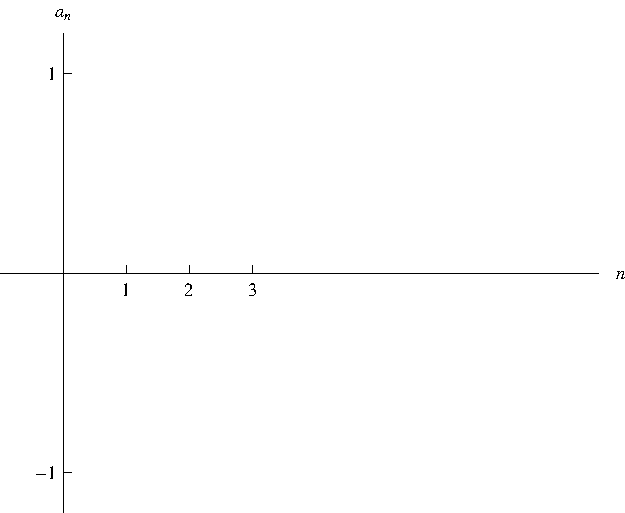
\includegraphics[height=4cm]{sequences/pictures/12-01-ex7a.pdf}%
}%
\only<5->{%
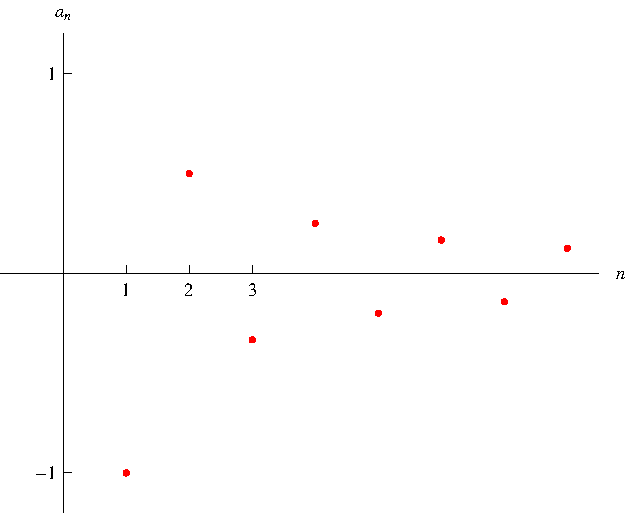
\includegraphics[height=4cm]{sequences/pictures/12-01-ex7b.pdf}%
}%
\column{.5\textwidth}
\[
\uncover<2->{%
\lim_{n\to\infty}\left| \frac{(-1)^n}{n}\right| = %
}%
\uncover<3->{%
\lim_{n\to\infty} \frac{1}{n} = %
}%
\uncover<4->{%
0%
}%
\]
\uncover<5->{%
Therefore, by the corollary to the Squeeze Theorem,
\[
\lim_{n\to\infty}\frac{(-1)^n}{n} = 0%
\]
}%
\uncover<6->{%
Therefore $\left\{ \frac{(-1)^n}{n} \right\}$ is convergent.
}%
\end{columns}
\end{example}
\end{frame}
% end module sequence-ex7

%% begin module sequence-geometric-ex10
\begin{frame}
\begin{example}[Example 10, p. 717]
\begin{columns}[c]
\column{.6\textwidth}
For what values of $r$ is the sequence $\{ r^n\}$ convergent?

\uncover<2->{%
Consider the exponential function $y = r^x$.}%
\abovedisplayskip=0pt
\belowdisplayskip=0pt
\[
\uncover<2->{%
\lim_{x\to\infty}r^x = \left\{ \begin{array}{lll}
\uncover<4->{\alert<handout:0| 4>{\infty}} & \alert<handout:0| 3-4>{\textrm{ if }} & \alert<handout:0| 3-4>{r > 1}\\
\uncover<6->{\alert<handout:0| 6>{0}} & \alert<handout:0| 5-6>{\textrm{ if }} & \alert<handout:0| 5-6>{0 < r < 1}\\
\end{array}\right.}%
\]
\uncover<7->{Therefore}
\abovedisplayskip=0pt
\belowdisplayskip=0pt
\[
\uncover<7->{%
\lim_{n\to\infty}r^n = \left\{ \begin{array}{lll}
\uncover<8->{\alert<handout:0| 8>{\infty}} & \alert<handout:0| 7-8>{\textrm{ if }} & \alert<handout:0| 7-8>{r > 1}\\
\uncover<10->{\alert<handout:0| 10>{0}} & \alert<handout:0| 9-10>{\textrm{ if }} & \alert<handout:0| 9-10>{0 < r < 1}\\
\end{array}\right.}%
\]
\uncover<11->{Also, $\displaystyle \alert<handout:0| 11-12>{\lim_{n\to\infty}1^n = \uncover<12->{1}}$ and $\displaystyle \alert<handout:0| 13-14>{\lim_{n\to\infty}0^n = \uncover<14->{0}}$.}

\uncover<15->{If $-1 < r < 0$, then $0 < |r| < 1$, and
\abovedisplayskip=0pt
\belowdisplayskip=0pt
\[
\lim_{n\to\infty} |r^n| = \lim_{n\to\infty}|r|^n = 0 
\]
Therefore $\displaystyle \lim_{n\to\infty}r^n = 0$.}

\uncover<16->{If $r < -1$, then $r^n$ diverges, just like $(-1)^n$.}
\column{.4\textwidth}
\ \only<handout:0| -7>{%
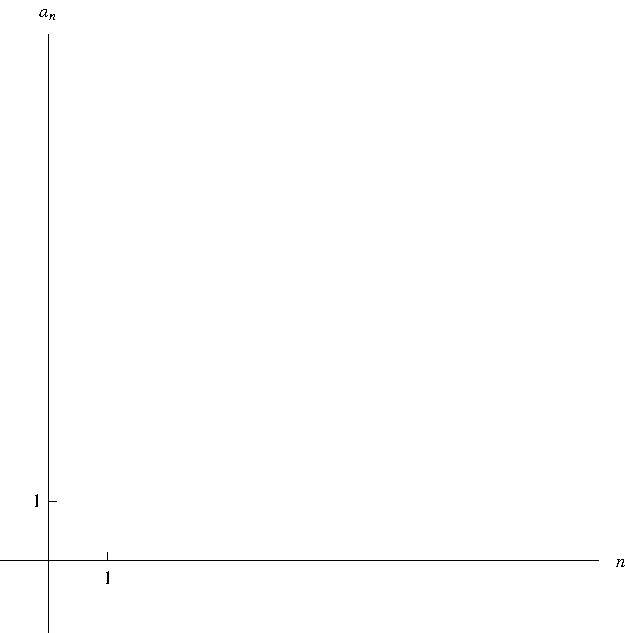
\includegraphics[height=3.8cm]{sequences/pictures/12-01-ex10a.pdf}%
}%
\only<handout:0| 8-9>{%
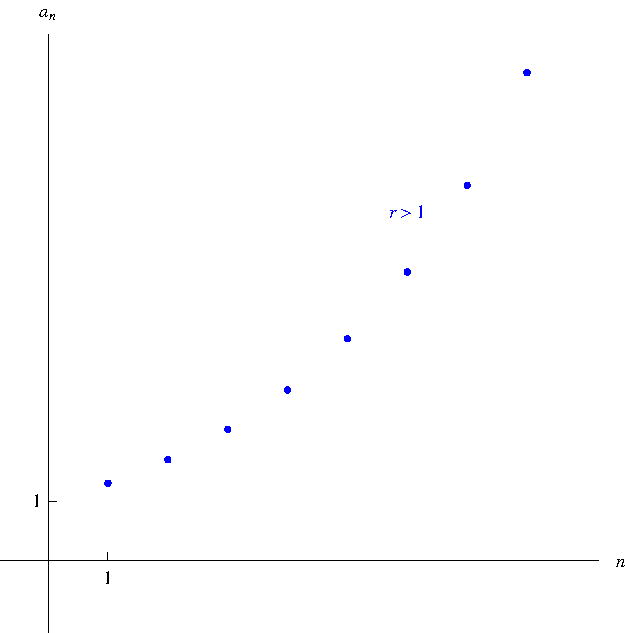
\includegraphics[height=3.8cm]{sequences/pictures/12-01-ex10b.pdf}%
}%
\only<handout:0| 10-11>{%
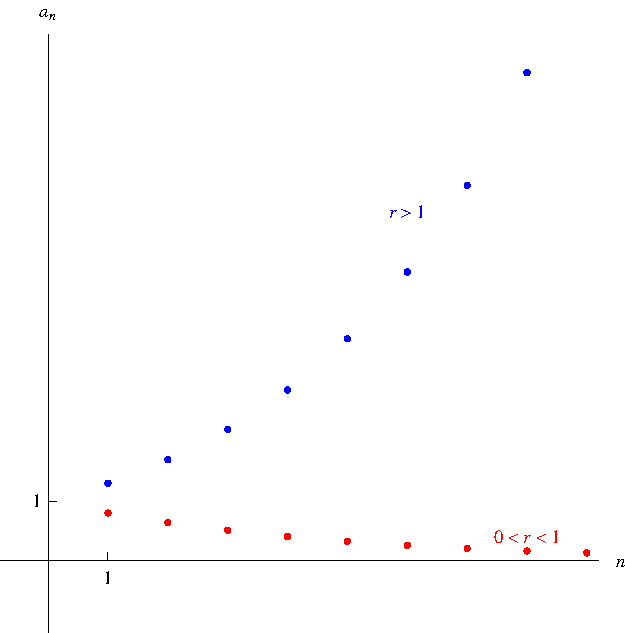
\includegraphics[height=3.8cm]{sequences/pictures/12-01-ex10c.pdf}%
}%
\only<12->{%
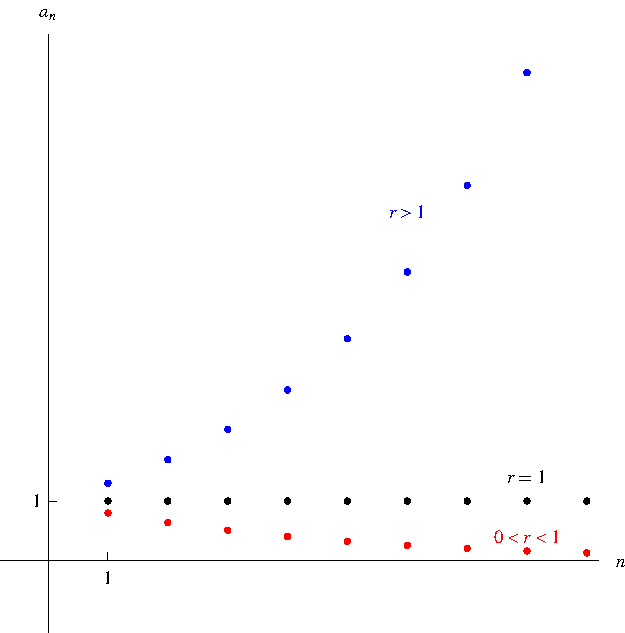
\includegraphics[height=3.8cm]{sequences/pictures/12-01-ex10d.pdf}%
}%

\ \only<handout:0| -14>{%
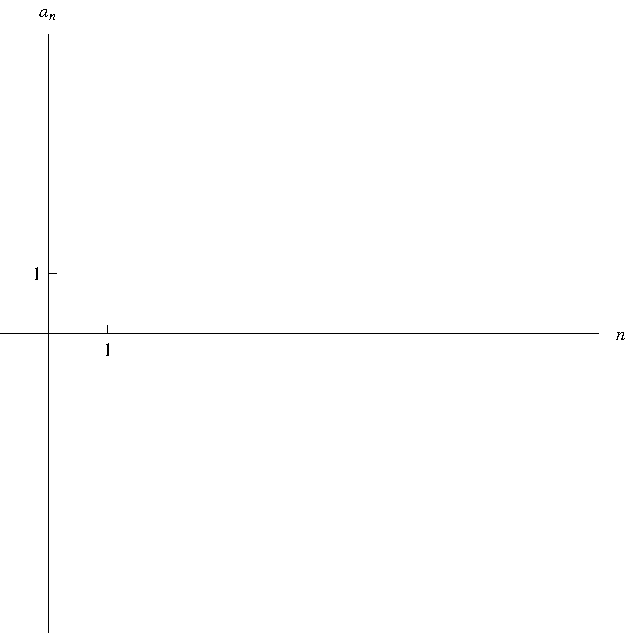
\includegraphics[height=3.8cm]{sequences/pictures/12-01-ex10e.pdf}%
}%
\only<handout:0| 15>{%
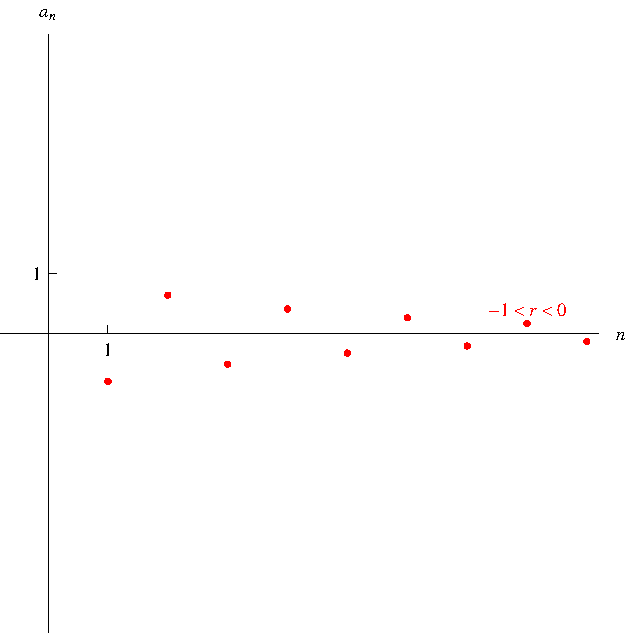
\includegraphics[height=3.8cm]{sequences/pictures/12-01-ex10f.pdf}%
}%
\only<16->{%
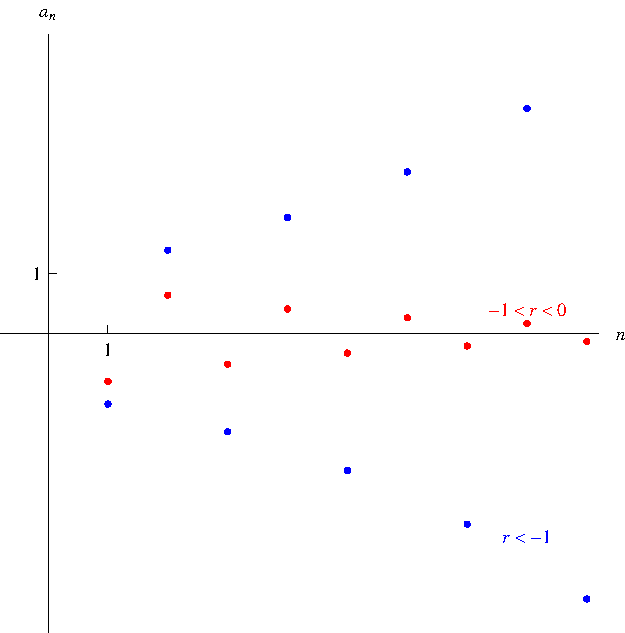
\includegraphics[height=3.8cm]{sequences/pictures/12-01-ex10g.pdf}%
}%
\end{columns}
\end{example}
\end{frame}
% end module sequence-geometric-ex10

% begin module sequence-plotting
\begin{frame}
\begin{columns}[c]
\column{.5\textwidth}
\ \only<handout:0| -2>{%
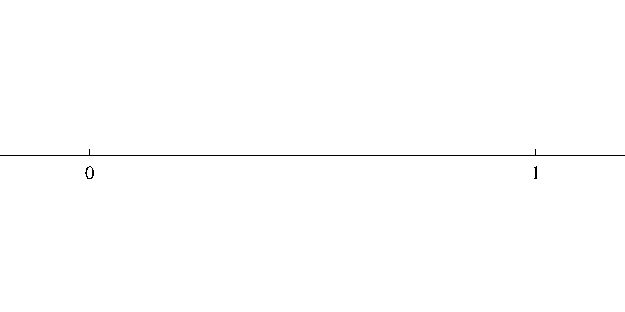
\includegraphics[width=5cm]{sequences/pictures/12-01-numberlinea.pdf}%
}%
\only<handout:0| 3>{%
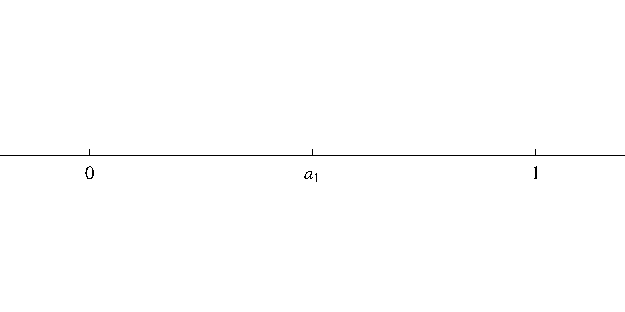
\includegraphics[width=5cm]{sequences/pictures/12-01-numberlineb.pdf}%
}%
\only<handout:0| 4>{%
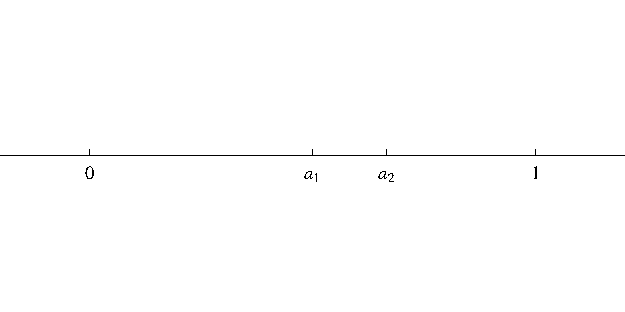
\includegraphics[width=5cm]{sequences/pictures/12-01-numberlinec.pdf}%
}%
\only<handout:0| 5>{%
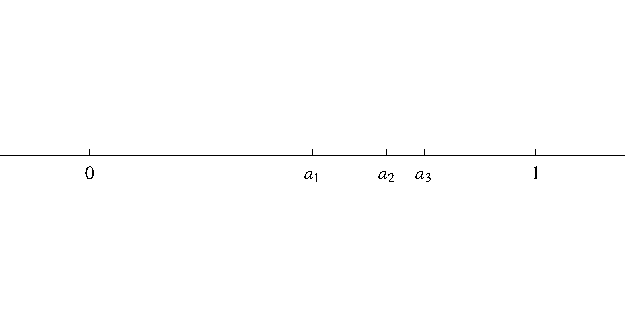
\includegraphics[width=5cm]{sequences/pictures/12-01-numberlined.pdf}%
}%
\only<handout:0| 6>{%
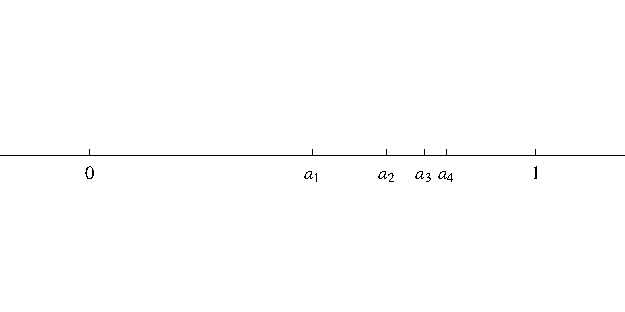
\includegraphics[width=5cm]{sequences/pictures/12-01-numberlinee.pdf}%
}%
\only<handout:0| 7>{%
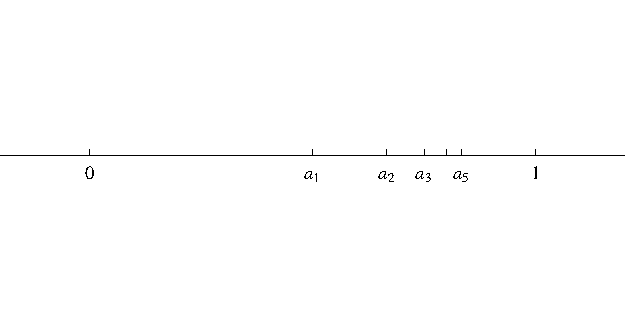
\includegraphics[width=5cm]{sequences/pictures/12-01-numberlinef.pdf}%
}%
\only<handout:0| 8>{%
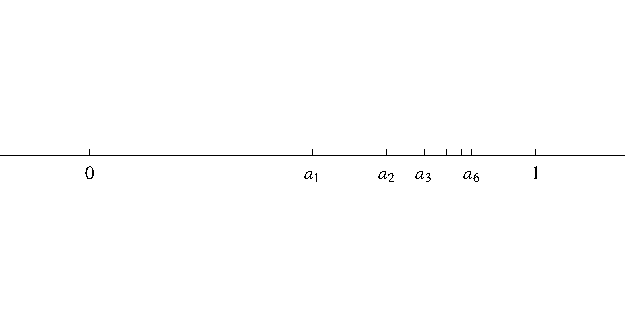
\includegraphics[width=5cm]{sequences/pictures/12-01-numberlineg.pdf}%
}%
\only<handout:0| 9>{%
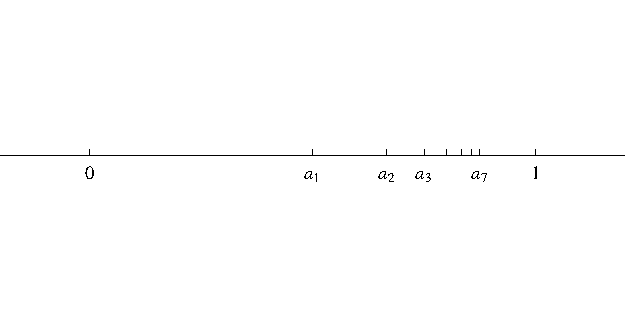
\includegraphics[width=5cm]{sequences/pictures/12-01-numberlineh.pdf}%
}%
\only<handout:0| 10>{%
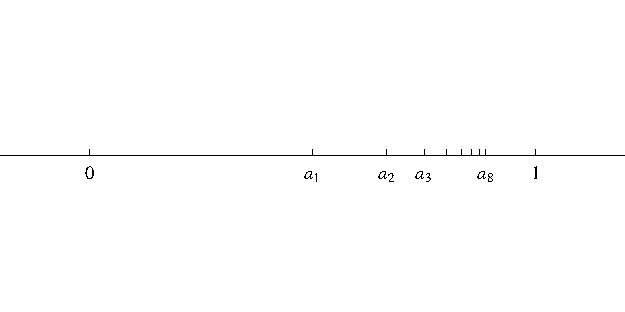
\includegraphics[width=5cm]{sequences/pictures/12-01-numberlinei.pdf}%
}%
\only<11->{%
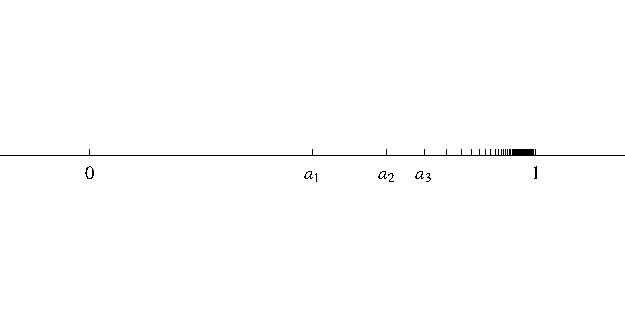
\includegraphics[width=5cm]{sequences/pictures/12-01-numberlinej.pdf}%
}%

Number line

\fcEvalToInt{3-1}

\column{.5\textwidth}
\begin{pspicture}(-0.5, -0.5)(4, 1.4)
\tiny
\fcAxesStandard{-0.5}{-0.5}{4}{1.4}
\fcYTickWithLabel{1}{$1$}
\rput[tl](4.1, -0.1){$n$}
\rput[rb]( -0.1, 1.45){$a$}
\multido{\na=2+1}{8}{%
\only<na->{\fcXTickWithLabel{\fcEvalToInt{\na-1}}{$\na$}}
}%
\end{pspicture}


\ \only<handout:0| -2>{%
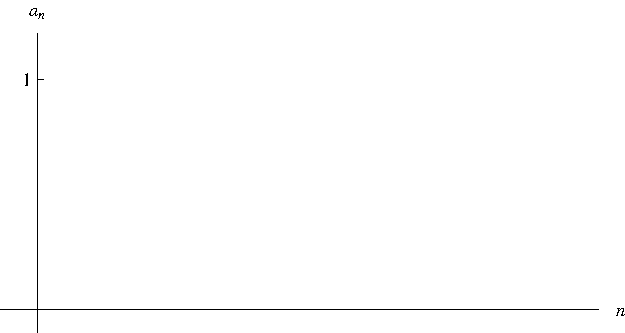
\includegraphics[width=6cm]{sequences/pictures/12-01-sequencegrapha.pdf}%
}%
\only<handout:0| 3>{%
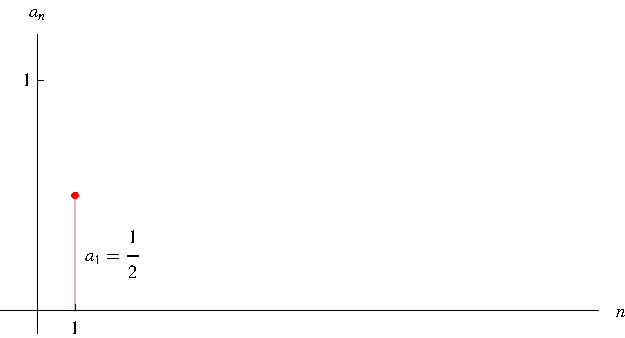
\includegraphics[width=6cm]{sequences/pictures/12-01-sequencegraphb.pdf}%
}%
\only<handout:0| 4>{%
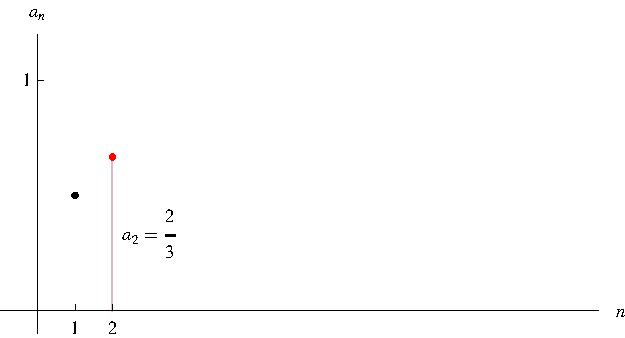
\includegraphics[width=6cm]{sequences/pictures/12-01-sequencegraphc.pdf}%
}%
\only<handout:0| 5>{%
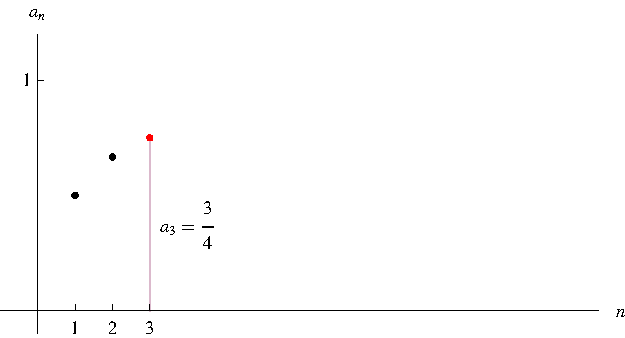
\includegraphics[width=6cm]{sequences/pictures/12-01-sequencegraphd.pdf}%
}%
\only<handout:0| 6>{%
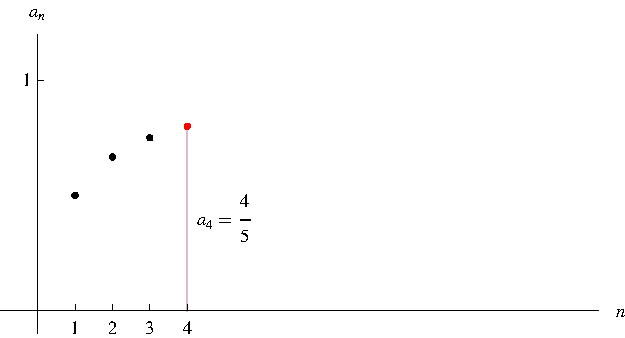
\includegraphics[width=6cm]{sequences/pictures/12-01-sequencegraphe.pdf}%
}%
\only<handout:0| 7>{%
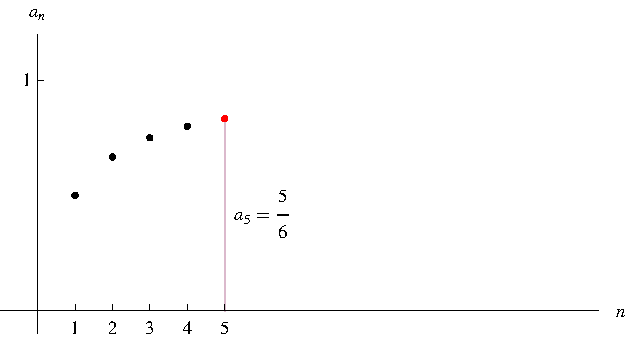
\includegraphics[width=6cm]{sequences/pictures/12-01-sequencegraphf.pdf}%
}%
\only<handout:0| 8>{%
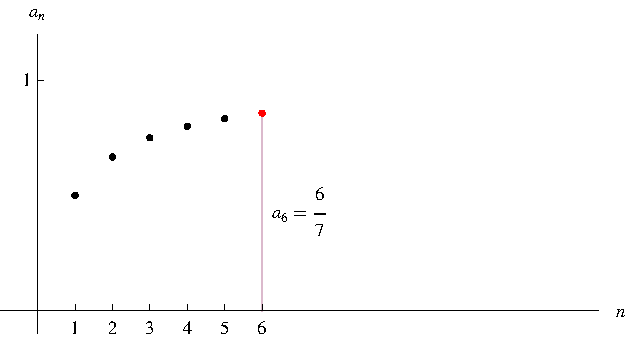
\includegraphics[width=6cm]{sequences/pictures/12-01-sequencegraphg.pdf}%
}%
\only<handout:0| 9>{%
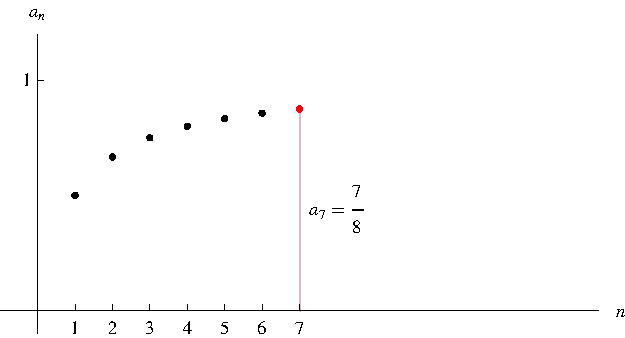
\includegraphics[width=6cm]{sequences/pictures/12-01-sequencegraphh.pdf}%
}%
\only<handout:0| 10>{%
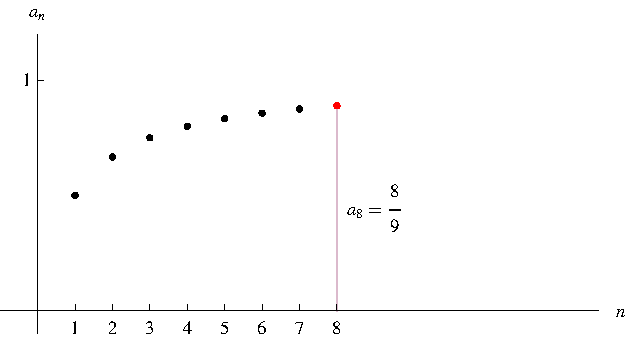
\includegraphics[width=6cm]{sequences/pictures/12-01-sequencegraphi.pdf}%
}%
\only<11->{%
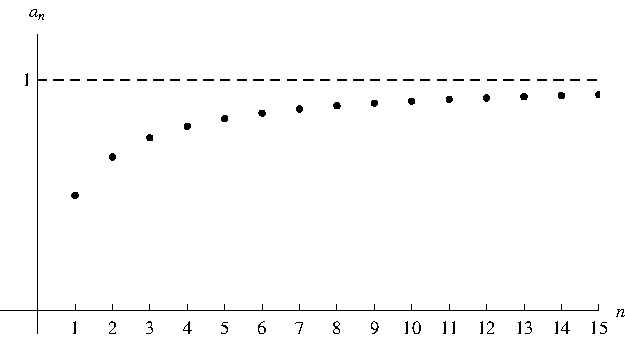
\includegraphics[width=6cm]{sequences/pictures/12-01-sequencegraphj.pdf}%
}%

Cartesian coordinates
\end{columns}
\begin{itemize}
\item  The sequence $\left\{ \frac{n}{n+1}\right\}$ can be plotted on a number line or using Cartesian coordinates.
\item<12->  From the pictures, the terms in the sequence appear to approach $1$ as $n$ gets larger.
\item<13->  \alert<handout:0| 13-14>{$1 - \frac{n}{n+1} =$ \uncover<14->{$\frac{1}{n+1}$.}}
\item<15->  This can be made arbitrarily small by choosing $n$ large enough.
\item<16->  We express this by writing $\lim_{n\to\infty}\frac{n}{n+1} = 1$.
\end{itemize}
\end{frame}
% end module sequence-plotting


%%begin module area-under-hyperbola-ex1

\begin{frame}
Recall Euler substitution: $x=\frac12\left(\frac{1}{t}- t \right)$, $\alert<2>{\sqrt{x^2+1}=\frac{1}2\left(\frac 1 t +t\right)}$, $\alert<12,13,14>{ t=\sqrt{x^2+1}-x} $, $\alert<3>{ \diff x=-\frac12 \left(\frac1{t^2} +1\right)\diff t}$.
\begin{example}
$
\begin{array}{rcl}
\displaystyle \int \alert<2>{ \sqrt{x^2+1}} \alert<3>{\diff x} \vphantom{ \frac{1}{8}\left(\frac{1}{ (\sqrt{ x^2 +1} -x)^2} - (\sqrt{x^2+1}- x)^2 \right) } &=&
\displaystyle
\only<1-16>{
\uncover<2->{ \alert<3>{-} \int  \alert<2>{\alert<4>{\frac12} \left(\alert<5,6>{\frac1t} +\alert<7,8>{t}\right)} \alert<3>{\alert<4>{ \frac{1}{2}} \left(\alert<5,7>{ \frac 1 {t^2}} +\alert<6,8>{1} \right)\diff t}} \\
\uncover<4->{ &=&\displaystyle -\alert<4>{ \frac 1 4} \alert<9,10,11>{ \int} \left(\alert<5>{ \alert<9>{ \frac{ 1 }{ t^3}}} + \alert<6,7,10>{2\frac{1}t} + \alert<8,11>{t} \right) \alert<9,10,11>{ \diff t} } \\
\uncover<9->{&=&\displaystyle \alert<15>{-\frac{1}4} \left( \alert<9>{ \alert<15>{ -}\frac{ \alert<12>{ t^{-2}}}{\alert<15>{2}}} +\alert<10>{ \alert<15>{2} \ln\alert<14>{ |t|} }+ \alert<11>{\frac{\alert<13>{ t^2}}{\alert<15>{2}}} \right)+C}\\
\uncover<12->{&=&}
}
\uncover<12->{\displaystyle \only<1-24>{  \alert<16,17,18,24>{ \alert<15>{\frac{1}{8}} \left(\frac{1}{\alert<12>{ (\sqrt{ x^2 +1} -x)^2}} - \alert<13>{\left(\sqrt{x^2+1}- x\right)^2} \right) } }}\only<25->{
\alert<25>{ \frac{1}{2}x\sqrt{x^2+1}}
} {~~~~~~~~~~~~~~~~~~~~~~~~~~~~~~~~~~~~~~~~~~~~~~~~~~~~~~}  \\
\uncover<12->{ && \displaystyle \alert<16,17>{ \only<1-30>{\alert<15>{ -}} \only<31->{\alert<31>{+} } \alert<15>{ \frac12}  \alert<26,30>{\ln \left( \alert<14>{ \sqrt{x^2+1} \only<1-30>{-}\only<31->{\alert<31>{+} } x} \right)} +C}}
\end{array}
$

\noindent \only<17-25>{The answer is good. However, let's simplify.

\noindent
\uncover<18->{
$
\begin{array}{l}
\phantom{=}
\displaystyle \alert<18>{ \frac{1}{(\sqrt{x^2+1}-x)^2}- \left( \sqrt{ x^2+1 }-x\right)^2} \\
\uncover<19->{= \displaystyle \frac{ \alert<19>{(\sqrt{x^2+1} +x )^2} }{ ( \sqrt{x^2 +1} -x )^2  	\alert<19>{(\sqrt{x^2+1}+x)^2} } - \left(\sqrt{x^2+1}-x\right)^2} \\
\uncover<20->{ =\displaystyle \frac{(\sqrt{x^2+1}+x)^2}{ \alert<20>{ \alert<21,22>{((\sqrt{x^2 +1 } )^2 -x^2 )^2 } \uncover<21,22>{\alert<21,22>{=1}} } } - \left( \sqrt{x^2 +1 } -x \right)^2} \\
\displaystyle \uncover<22->{=\left(\sqrt{x^2+1}+x\right)^2-\left( \sqrt{ x^2 + 1 } -x\right)^2} \uncover<23->{ = \alert<24,25>{ 4x\sqrt{x^2+1}}}
\end{array}
$
} %uncover<18->
} %only<17-25>

\only<26->{
The last expression can be transformed to:
\[
\begin{array}{rcl}
\displaystyle
\alert<26>{\ln} \left(\frac{\alert<26,28>{\left(\sqrt{x^2+1}-x\right)} \uncover<27->{ \alert<27,28>{\left( \sqrt{x^2+1}+ x \right)} }}{ \uncover<27->{ \alert<27>{ \sqrt{x^2 +1} +x}}} \right)
&=& \displaystyle \uncover<28->{\alert<29>{ \ln \left( \frac{\alert<28>{ 1} }{ \sqrt{x^2+1}+x}\right)} }\\ \uncover<29->{&=&\alert<29,30,31>{ -\ln \left(\sqrt{x^2+1}+x\right)}}
\end{array}
\]
}
\end{example}

\vspace{8cm}
\end{frame}

\begin{frame}
\begin{example}
Find the area locked b-n the hyperbolas $\alert<2,3>{ y=\pm \sqrt{ x^2+1}}$ and $x=\pm 2\sqrt{ 2}$.
\begin{columns}
\column{.5\textwidth}
\psset{xunit=0.7cm, yunit=0.7cm}
\begin{pspicture}(-3.328427, -3)(3.328427,3)
\psframe*[linecolor=white](-3.328427,-3)(3.328427,3)
\tiny
\uncover<31->{
\pscustom*[linecolor=\fcColorAreaUnderGraph]{
\psplot[linecolor=\fcColorGraph, plotpoints = 1000 ] {-2.828427} {2.828427}{1 x 2 exp add 0.5 exp }
\psline[linecolor=\fcColorGraph](2.828427,-3)(2.828427,3)
\psplot[linecolor=\fcColorGraph, plotpoints=1000] { 2.828427 } {-2.828427}{1 x 2 exp add 0.5 exp -1 mul }
\psline[linecolor=\fcColorGraph](-2.828427,-3)(-2.828427,3)
}
}
\uncover<1-26,28->{
\psaxes[arrows=<->,ticks=none, labels=none](0,0)(-3,-3)(3,3)
}
\psline[linecolor=red!1](3.301,2)(3.302,2)
\psline[linecolor=red!1](-3.301,2)(-3.302,2)

%Function formula: - (x^{2}+1)^{1/2}
\psplot[linecolor=\fcColorGraph, plotpoints=1000]{-2.828427}{2.828427}{1 x 2 exp add 0.5 exp -1 mul }
\uncover<3-4>{\rput[tl](-2.2, -2.4){ \alert<3>{ $y= - \sqrt{ x^2 +1 }$}}}

%Function formula: (x^{2}+1)^{1/2}
\psplot[linecolor=\fcColorGraph, plotpoints=1000]{-2.828427}{ 2.828427 }{1 x 2 exp add 0.5 exp }
\uncover<2-4>{\rput[bl](-2.1, 2.4){\alert<2>{ $y=\sqrt{ x^2 +1} $}}}

\uncover<29->{
\psline[linecolor=\fcColorGraph](-2.828427,3)(-2.828427,-3)
}
\uncover<30->{
\psline[linecolor=\fcColorGraph](2.828427,3)(2.828427,-3)
}
\uncover<25-27>{
\psline{<->}(-2.9,2.9)(2.9,-2.9)
\rput[t](-2.1, 1.7){$\begin{array}{l} \alert<25>{v=0} \\\uncover<1-26>{\alert<25>{y+x=0}} \end{array}$}
}
\uncover<15-27>{
\psline{<->}(-2.9,-2.9)(2.9,2.9)
\rput[b](-2.1, -1.9){$\begin{array}{l} \uncover<1-26>{ \alert<15>{ y-x=0 }}\\\uncover<16->{\alert<16>{u=0}} \end{array}$}
}
\uncover<17-26>{
\fcFullDot{1.4}{1.4}
\rput[l]( 1.6, 1.4){$(\frac{y+x}{2},\frac{y+x}{2})$}
}
\uncover<14-26>{
\fcFullDot{0.6}{2.2}
\rput[lb](0.65, 2.2){$(x,y)$}
}
\uncover<26>{
\psline(0.6,2.2)(-0.8,0.8)
\psline(-0.7, 0.9)(-0.6, 0.8)(-0.7, 0.7)
\rput[rb](-0.3, 1.3){\alert<26>{$v$}}
}
\uncover<18-26>{
\psline(0.6,2.2)(1.4, 1.4)
\psline(1.3, 1.5)(1.2,1.4)(1.3, 1.3)
}
\uncover<23-26>{
\rput[tr](0.95, 1.8){\alert<23>{$u$}}
}
\uncover<14-26>{
\fcFullDot{2.2}{0.6}
\rput[lt]( 2.2, 0.65){$(y,x)$}
}
\end{pspicture}

\vbox to 3.0cm {
\uncover<18->{\alert<18>{
\uncover<22->{\alert<22>{Signed}} distance b-n $(x,y)$ and line $u=0$ equals}}
\only<1-23>{
$\uncover<19->{\uncover<22->{\alert<22>{\pm}} \alert<19>{ \sqrt{ \alert<20>{ \left(x-\frac{(x+y)}{2} \right)^2+ \left( y- \frac{(x+y )}{2} \right)^2}}}}
$
$\uncover<20->{=\uncover<22->{\alert<22>{\pm}} \sqrt{ \alert<20>{ \frac{1}{2}(y-x)^2 }}} \uncover<21->{= \alert<21>{ \uncover<1-21>{\pm} \alert<23>{ \frac{\sqrt{2 }}{ 2 } ( y-x)}}} \uncover<23>{ \alert<23>{=}}$
} %only<1-23>
\uncover<23->{ \alert<23,24>{$u $}.}
\only<24->{\uncover<25->{
Similarly compute that \alert<26>{signed distance b-n $(x,y)$ and the \alert<25>{line $v=0$} equals $v$}.
\uncover<27->{$\Rightarrow$ $y^2-x^2=1$ is the \alert<27>{ hyperbola $v=\frac{1/2}{v}$} in the $(u,v)$-plane.}
}}

\vfil
} %vbox

\column {.5\textwidth}
\only<1-27>{
\uncover<4->{We studied $\alert<27>{v=\frac{1/2}{u}}$ is called a hyperbola:}\uncover<3->{ why do we call $y= \sqrt{ x^2 +1}$ hyperbola?} \uncover<5->{Compute:}
\[
\begin{array}{rcl}
\uncover<5->{\sqrt{x^2+1} &=& y}\\
\uncover<6->{ x^2+1 &=& y^2}\\
\uncover<7->{y^2-x^2&=&1}\\
\uncover<8->{\uncover<9>{\alert<9>{\frac{1}{2}}} \uncover<10->{\alert<10,11>{\frac{\sqrt{2}}{2}}} \alert<11>{(y-x)} \uncover<10->{\alert<10,12>{\frac{\sqrt{2}}{2}}} \alert<12>{(y+x)}&=&\uncover<9->{\alert<9>{\frac{1}{2}}} \uncover<8>{1}}\\
\uncover<11->{\alert<11>{u}\alert<12>{v}&=& \frac{1}{2}}\\
\uncover<13->{\alert<27>{v}&\alert<27>{=}& \alert<27>{\frac{1/2}{u}},}
\end{array}
\]
\uncover<11->{where $\begin{array}{|l}
\alert<11,16,23>{u=\frac{\sqrt{2}}{2} \left(y-x\right)}\\
\alert<12,25>{v=\frac{\sqrt{2}}{2}\left(y+x\right)}
\end{array}$. } \uncover<14->{Consider an arbitrary point $(x,y)$.}
} %only<1-27>
\only<28->{
The area in question is:
$
\begin{array}{l}
\displaystyle\phantom{=} \int \limits^{{{\uncover<28,29>{\alert<29>{ \textbf{?}}}\uncover<30->{\alert<30>{ 2\sqrt{2}}}}}}_{\uncover<28>{\alert<28>{\textbf{?}}}\uncover<29->{ -2\sqrt{2}}} 2\sqrt{x^2+1}\diff x \\
\displaystyle \uncover<32->{= \uncover<33->{\alert<33>{2}} \left[x\sqrt{x^2+1} \vphantom{\ln \left(\sqrt{x^2+1}+x\right) }\right.}\\
\displaystyle \uncover<32->{\left. \ln \left(\sqrt{x^2+1}+x\right)\right]^{2\sqrt{2}}_{\only<33->{\alert<33>{0}} \uncover<1-32>{-2\sqrt{2}}}}\\
\uncover<34->{=2\left(2\sqrt{2} \sqrt{(2\sqrt{2})^2+1}\right.} \\
\uncover<34->{\left.+ \ln \left(\sqrt{(2\sqrt{2})^2+1}+2\sqrt{2} \right) \right)}\\
\uncover<35->{=12\sqrt{2} +2\ln \left(3+2\sqrt{2}\right )}\\
\uncover<36->{\approx 20.496}
\end{array}
$
}
\end{columns}

\end{example}

\end{frame}

%end module area-under-hyperbola-ex1

%% begin module arcsin-ex1
\begin{frame}
\vskip -0.1cm
\begin{example}
\begin{columns}[t]
\column{.3\textwidth}
\hfil \hfil Find $\displaystyle \Arcsin \left( \frac{1}{2}\right)$.
\begin{itemize}
\item<2->  $\displaystyle \sin \left(\uncover<2-| handout:0>{\frac{\pi}{ 6}}\right) = \frac{1}{2}$.
\item<3->  $\displaystyle -\frac{\pi}{2} \leq \uncover<3-| handout:0>{\frac{\pi}{6}} \leq \frac{\pi}{2}$.
\item<4->  Therefore $ \Arcsin \left( \frac{1}{2}\right) = \uncover<3-| handout:0>{\frac{\pi}{6}}$.
\end{itemize}
\column{.7\textwidth}
\hfil \hfil Find $\displaystyle
\tan \left( \Arcsin \left( \frac{1}{3}\right) \right)
$.
\begin{itemize}
\item<5->  Let $\theta = \Arcsin \left(\frac{1}{3}\right)$, so $\sin \theta = \frac{ \alertNoH{6}{1}}{\alertNoH{7}{3}}$.
\item<6->  Draw a right triangle with  \alertNoH{6}{opposite side $1$} and \alertNoH{7}{hypotenuse $3$}.
\item<8-> Let the angle $\theta$ be as labeled. \uncover<9->{ Then $ \alertNoH{9,10}{\sin\theta= \frac{1 }{3}}$ \uncover<10->{and so $\alertNoH{10}{ \theta= \arcsin\left(\frac{1}{3}\right)}$}.}
\item<11->  \alertNoH{11-12}{Length of adjacent side $ =\worksheet{ \fcAnswer{12}{\sqrt{3^2-1^2}} \uncover<13->{ = \sqrt{8} = 2\sqrt{2}.}}$}
\item<14->  Then \alertNoH{ 14-15}{$\tan \left(\Arcsin \left(\frac{1}{3}\right)\right) = \fcAnswer{15}{ \frac{1}{ 2\sqrt{2}}.}$}
\end{itemize}

\vskip -0.1cm
\hfil\hfil \psset{xunit=1.5cm, yunit=1.5cm}
\begin{pspicture}(-0.2, -0.35)(3.2,1.05)
\small%
\fcBoundingBox{-0.2}{-0.35}{ 10 sqrt 0.3 add}{1.15}
\psline[linecolor=red!1](2.828427125, 1)(2.828427125, 1.01)
\psline[linecolor=red!1](0, -0.35)(0.001, -0.35)
\psdot[linecolor=white](3.1, 1.0)
\psdot[linecolor=white](-0.1, -0.3)
\uncover<6->{%
\psline(0,0)(! 10 sqrt 0)(! 10 sqrt  1)(0,0)
\psline(! 10 sqrt 0.1)(! 10 sqrt 0.1)(! 10 sqrt 0)
\rput[b](1.41, 0.55){$3$}
\rput[l](! 10 sqrt 0.05 add 0.5){$1$}
\rput(0.8, 0.13){$ \alertNoH{8}{\theta}$}
\fcAngle{0}{0.339837}{0.4}{}
}
\uncover<handout:0|6,9,15>{\psline[linewidth=2pt, linecolor=blue](! 10 sqrt 0)(! 10 sqrt  1)}%
\uncover<handout:0|15>{\psline[linewidth=2pt, linecolor=green](0,0)(! 10 sqrt 0)}%
\uncover<handout:0|7,9>{\psline[linewidth=2pt, linecolor=orange](! 0 0)(! 10 sqrt  1)}%
\uncover<11-| handout:0>{\rput[t](! 10 sqrt 2 div -0.1){$ \fcAnswerUncover{11}{13}{ 2 \sqrt{2}}$}}
\end{pspicture}
\end{columns}

\end{example}
\end{frame}
% end module arcsin-ex1


%% begin module integration-by-parts-ex4
\begin{frame}
\alertNoH{4,5,12,13}{Integration by parts:} $\displaystyle \int \alertNoH{6,14}{u} \diff \alertNoH{7,15}{v} = \alertNoH{6 ,14}{ u} \alertNoH{7,15}{v} - \int \alertNoH{7,15}{v} \diff \alertNoH{6,14}{u}.$


\begin{example}
$
\begin{array}{rcl}
\displaystyle \alertNoH{22}{ \int \alertNoH{2,3}{e^x} \sin x \alertNoH{2,3}{\diff x}}
\only<handout:1|1-20>{%
&\alertNoH{0}{=}&\displaystyle \uncover<2->{ \alertNoH{4,5}{\int \alertNoH{6}{\sin x}~ \alertNoH{2,3}{\diff \left(\alertNoH{7}{\fcAnswer{3}{ e^x}} \right)}}} \\
&\uncover<4->{\alertNoH{4,5}{=}} &\displaystyle \fcAnswer{5}{ \alertNoH{6}{(\sin x)}\alertNoH{7}{e^x} -\int \alertNoH{7}{e^x} \alertNoH{8,9}{\diff (\alertNoH{6}{\sin x})}} \\
\uncover<8->{ &\alertNoH{0}{=}&\displaystyle e^x \sin x - \int \alertNoH{10,11}{e^x}\fcAnswer{9}{ \cos x \alertNoH{10,11}{\diff x}}} \\
\uncover<10->{&\alertNoH{0}{=}&\displaystyle  e^x\sin x  - \alertNoH{12,13}{ \int \alertNoH{14}{\cos x} \alertNoH{10,11}{ \diff \left( \alertNoH{15}{\fcAnswer{11}{e^x}}\right)}}}\\
\uncover<12->{&\alertNoH{0}{=}&\displaystyle e^x \sin x  \alertNoH{16}{-} \left( \fcAnswer{13}{ (\alertNoH{14}{\cos x}) \alertNoH{15}{ e^x} \alertNoH{16}{-}  \int \alertNoH{15}{e^x} \alertNoH{17,18}{\diff (\alertNoH{14}{\cos x})}} \right)} \\
\uncover<16->{&\alertNoH{0}{=}&\displaystyle e^x\sin x - \cos x e^x  \alertNoH{16}{+} \int e^x \fcAnswerUncover{16}{18}{ ( \alertNoH{ 19}{-} \sin x)\diff x} }  \\
} %only<1-21>
\uncover<19->{ &\alertNoH{20,21}{=}&\alertNoH{20,21}{ \displaystyle e^x\sin x - \cos x e^x  \alertNoH{22}{ \alertNoH{ 19}{-}\int e^x \sin x \diff x}}} \\
\displaystyle \uncover<handout:2|22->{ \alertNoH{22}{\alertNoH{23}{2}\int e^x \sin x \diff x} &\alertNoH{0}{=}&\displaystyle e^x\sin x - \cos x e^x
}
\\
\uncover<handout:2|23->{\displaystyle \int e^x \sin x \diff x &\alertNoH{ 0 }{ =}&\displaystyle \frac{1}{ \alertNoH{23}{2} }\left( e^x\sin x - \cos x e^x\right) \uncover<24->{\alertNoH{24}{+C}}
}
\end{array}
$
\end{example}

\vskip 10cm
\end{frame}
% end module integration-by-parts-ex4


%% begin module partial-fractions-case2-ex4
\begin{frame}
\begin{example}
$
\begin{array}{@{\!\!}r@{\!}c@{}l}
\displaystyle \int \alertNoH{25}{ \frac{x^{4}+x^{3}-4x^{2}+4x }{x^3-x^2-x+1} }\diff x%
& \uncover<25->{ = } & %
\displaystyle \uncover<25->{%
\alertNoH{29,30}{ \alertNoH{31,32,33,34}{\int} \left(\alertNoH{25}{ \alertNoH{26,31}{x + 2} + \alertNoH{27} {  \alertNoH{32}{\frac{\alertNoH{28}{ 1}}{x-1}} + \alertNoH{33}{\frac{\alertNoH{28}{1}}{(x-1)^2}} \alertNoH{28}{-} \alertNoH{34}{\frac{\alertNoH{28}{2}}{x+1}}}} \right) \alertNoH{31,32,33,34}{\diff x}}
}\\%
& \uncover<29->{\alertNoH{29}{ =} } & %
\fcAnswer{30}{ \alertNoH{31}{\frac{x^2}{2} + 2x} + \alertNoH{32}{\ln |x-1|}  \alertNoH{33}{-\frac{1}{x-1}} -\alertNoH{34}{2\ln |x+1|} + K}%
\end{array}
$
\begin{itemize}
\item<2->  Divide: $\frac{x^{4}+x^{3}-4x^{2}+4x}{x^3-x^2-x+1} = x + 2 +  \frac{-x^{2}+5x -2}{\alertNoH{5}{x^3-x^2-x+1}} \uncover<5->{ = \alertNoH{26}{x + 2} + \alertNoH{6, 27}{\frac{- x^{ 2} +5x -2}{ \alertNoH{5}{(x-1)^2( x+1)}}}.}$
\item<3->  Factor denominator: $\alertNoH{5}{\fcQuestion{3}{x^3-x^2-x+1 =}\fcAnswer{4}{ (x-1)^2 (x+ 1).}}$
\item<6-> Set up the partial fraction decomposition:
$\renewcommand{\arraystretch}{1.4}
\begin{array}{rcl}
\displaystyle \uncover<6->{\alertNoH{6,7,27}{ \frac{-x^{2}+5x -2}{ \alertNoH{8,9,10}{ (x-1)^2(x+1)}}}}& % 
\uncover<6->{ \alertNoH{6,7}{=} } & %
\displaystyle  \fcAnswer{7}{\frac{ \alertNoH{28}{A}}{ \alertNoH{8}{x-1}} + \frac{\alertNoH{28}{ B}}{ \alertNoH{9}{( x-1)^2}} + \frac{\alertNoH{28}{C}}{\alertNoH{10}{x+1}}}\\%
\uncover<8->{-\alertNoH{12,16,20}{x}^{2}+5\alertNoH{12,16,20}{x} -2}& 
\uncover<8->{ = } & %
\uncover<8->{A \alertNoH{8}{ (\alertNoH{15,16}{\alertNoH{20}{x} -1})(\alertNoH{11,12}{\alertNoH{20}{x}+1})} + B\alertNoH{9}{ ( \alertNoH{11,12}{\alertNoH{16,20}{x}+1})} + C\alertNoH{10}{ ( \alertNoH{15,16}{\alertNoH{12,20}{x}-1})^2}}\\%
\end{array}
$

\item<11->  Plug-in $\alertNoH{11,12}{ x=-1}$: \uncover<12->{$-(\alertNoH{12}{-1})^2+5(\alertNoH{12}{-1})-2 = C(\alertNoH{12}{-1}-1)^2 $ \uncover<13->{$\Rightarrow \alertNoH{21,22,28}{ \alertNoH{13,14}{C=}\fcAnswer{14}{ -2} }$.}}
\item<15->  Plug-in $\alertNoH{15,16}{x=1}$: \uncover<16->{$-( \alertNoH{16}{1})^2+\alertNoH{16}{1}\cdot 5-2 = B(\alertNoH{16}{1}+1) $ \uncover<17->{$\Rightarrow \alertNoH{21,22,28}{ \alertNoH{17,18}{B =} \fcAnswer{18}{1} } $.}}
\item<19->  Plug-in $\alertNoH{19,20}{x=0}$: \uncover<20->{$-2 = A(\alertNoH{20}{0}-1)(\alertNoH{20}{0}+1) +  \uncover<22->{\alertNoH{22}{1\cdot}} \uncover<handout:0 | 20,21>{\alertNoH{21}{B}}(\alertNoH{20}{0}+1) + \uncover<22->{\alertNoH{22}{(-2)}} \uncover<handout:0 | 20,21>{\alertNoH{21}{C}} (\alertNoH{20}{0}-1)^2}$  \uncover<23->{$\Rightarrow \alertNoH{28}{\alertNoH{23,24}{A =} \fcAnswer{24}{1} }$.}
\end{itemize}

\end{example}
\end{frame}
% end module partial-fractions-case2-ex4


%% begin module trig-integrals-tann-secm-strategy-and-tan-and-sec
\begin{frame}
\vskip -0.1cm
\begin{example}
$\begin{array}{rcll|l}
\displaystyle \int \tan x \diff x&\uncover<2->{=}&\displaystyle \uncover<2->{\int \frac{\alertNoH{3,4}{ \sin x}}{\cos x} \alertNoH{3,4}{\diff x} } \uncover<3->{= \int \frac{1}{ \alertNoH{5}{\cos x}}\alertNoH{3,4}{ \diff (\fcAnswer{4}{ \alertNoH{6}{-} \alertNoH{5}{\cos x}})}} \uncover<5->{&& \text{Set }\alertNoH{5,8}{u = \cos x}}\\
& \uncover<5->{=}&\displaystyle  \uncover<5->{\alertNoH{6}{-} \alertNoH{7}{\int \frac{\diff \alertNoH{5}{u}}{\alertNoH{5}{u}}}} \uncover<7->{ = }  \uncover<7->{- \alertNoH{7}{\ln |\alertNoH{8}{u}|} + C}\\
& \uncover<8->{ = } &\displaystyle  \uncover<8->{\alertNoH{9}{-}\ln |\alertNoH{8,9}{\cos x}| + C} \uncover<9->{ = } \displaystyle  \uncover<9->{\ln |\alertNoH{9}{\sec x}| + C}\\
\end{array}
$
\end{example}
\uncover<10->{The following can be/was computed via $x=2\arctan t$. \uncover<11->{Alternatively:}}
\begin{example}
$
\begin{array}{rcll|l}
\displaystyle \uncover<10->{\int \sec x \diff x} &\uncover<11->{=}&\displaystyle  \uncover<11->{\int \alertNoH{12,13}{\sec x}\frac{\alertNoH{11}{(\alertNoH{12}{\sec x} + \alertNoH{13}{\tan x})}}{\alertNoH{11}{(\sec x + \tan x)}}\diff x} \\
&\uncover<12->{=}& \displaystyle \uncover<12->{\int \frac{ \alertNoH{12,14}{\sec^2 x }+ \alertNoH{13,15}{\sec x \tan x}}{\sec x + \tan x}\alertNoH{14,15}{\diff x}}\\
&\uncover<14->{=}& \displaystyle \uncover<14->{\int \frac{ \alertNoH{14, 15}{\diff} (\alertNoH{16}{\alertNoH{14}{\tan x} + \alertNoH{15}{ \sec x}})}{\alertNoH{16}{\sec x + \tan x}}} \uncover<16->{&& \text{Set } \alertNoH{16,18}{u = \sec x + \tan x}}\\
&\uncover<16->{=}& \displaystyle \uncover<16->{\alertNoH{17}{ \int \frac{\diff \alertNoH{16}{u}}{\alertNoH{16}{u}}}}
\uncover<17->{=} \uncover<17->{\alertNoH{17}{\ln |\alertNoH{18}{u}|} + C}\\
&\uncover<18->{=}& \uncover<18->{\ln |\alertNoH{18}{\sec x + \tan x}| + C .}\\
\end{array}
$
\end{example}

\end{frame}
% end module trig-integrals-tann-secm-strategy-and-tan-and-sec


%% begin module trig-substitutions-ex3
\begin{frame}
\begin{example} 
$
\begin{array}{@{\!}r@{}c@{}l@{}l@{~}|l}
\displaystyle \int \frac{1}{x^2 \sqrt{x^2+\alertNoH{2}{9}}} \diff x&\uncover<2->{=}&\uncover<2->{\displaystyle  \int \frac{1}{\alertNoH{5}{x}^2 \alertNoH{2}{3}\sqrt{\left(\alertNoH{3,5}{\frac{x}{\alertNoH{2}{3}}} \right)^{\alertNoH{2}{2}}+\alertNoH{2}{1}}}\diff \alertNoH{5}{x}} \uncover<3->{&&
\begin{array}{@{}r@{~}c@{~}l}
&&\text{Set } \\
\alertNoH{3,5}{\frac{x}{\alertNoH{4}{3}}}&\alertNoH{3,5}{=}& \alertNoH{3,5}{\cot \theta}\\ 
\uncover<4->{\alertNoH{5}{x}&\alertNoH{5}{=}& \alertNoH{5}{\alertNoH{4}{3}\cot\theta}}
\end{array}} \\
&\uncover<5->{=}&\displaystyle \uncover<5->{\int \frac{1}{(\alertNoH{5}{\alertNoH{6}{3} \cot\theta})^{\alertNoH{6}{2}} \alertNoH{6}{3} \sqrt{\alertNoH{7,8}{ \alertNoH{5}{\cot}^2\alertNoH{5}{\theta}+1}} }\alertNoH{9,10}{\diff (\alertNoH{5}{3\cot \theta})}} \uncover<3->{&& \theta \in (0, \pi)}\\
&\uncover<6->{=}&\displaystyle \uncover<6->{ \int \frac{ 1}{\alertNoH{6,11}{27} \cot^{2}\theta \alertNoH{12}{\sqrt{ \fcAnswerUncover{6}{8}{\csc^2\theta}}}} \alertNoH{9,10}{\left(\fcAnswerUncover{6}{10}{-\alertNoH{11}{3}\csc^2\theta} \right)\diff \theta }}\uncover<12->{ && \begin{array}{@{}l}\theta\in(0,\pi)\Rightarrow \\ \alertNoH{12}{\csc\theta>0} \end{array}}\\
&\uncover<11->{=}&\displaystyle \uncover<11->{\alertNoH{11}{\frac{1}{9}} \int \alertNoH{13}{\frac{ -\csc^2\theta }{ \cot^{2}\theta \alertNoH{12}{\csc\theta}}} \diff \theta} \\
&\uncover<13->{=}&\displaystyle\uncover<13->{ \frac{1}{9}\int \alertNoH{13}{ \frac{ \alertNoH{14,15}{-\sin\theta }}{\cos^2\theta}} \alertNoH{14,15}{\diff \theta} }
\uncover<14->{=\frac{1}{9}\int \frac{1}{\alertNoH{16}{\cos}^2\alertNoH{16}{\theta}} \alertNoH{14,15}{\diff(\fcAnswer{15}{\alertNoH{16}{ \cos\theta}})}} \uncover<16->{ &&\!\text{Set } \alertNoH{16,19}{u=\cos\theta}}\\
&\uncover<16->{=}&\uncover<16->{\displaystyle \alertNoH{17,18}{\frac{1}{9} \int \frac{\diff \alertNoH{16}{u}}{\alertNoH{16}{u}^2}}} \uncover<17->{=   \fcAnswer{18}{ -\frac{\alertNoH{19}{1}}{9\alertNoH{19}{u}}}+C} \uncover<19->{=-\frac{ \alertNoH{19-24}{ \sec \theta} }{9} +C } 
\uncover<20->{&&
\raisebox{-0.5cm}{
\psset{xunit=0.3cm, yunit=0.3cm}
\begin{pspicture}(-0.8,-0.8)(4.6,3.2)
\tiny
\fcBoundingBox{-1}{-0.8}{4.6}{3.2}
\psline(0,0)(4, 0)(4,3)(0,0)
\psline(3.8,0)(3.8, 0.2)(4,0.2)
\fcAngle{0}{3 4 div ATAN}{0.8}{}
\rput[bl](1, 0.2){$\alertNoH{20}{\theta}$}
\rput[l](4.2, 1.5){$\fcAnswer{21}{\alertNoH{23}{3}}$}
\rput[t](2, -0.2){$\fcAnswer{21}{\alertNoH{23,24}{x}}$}
\rput[br](2, 1.5){$\uncover<23->{\alertNoH{23,24}{\sqrt{x^2+9}}} \fcAnswer{23}{ }~$}
%bounding box for pdflatex compilation:
\psline[linecolor=red!1](-0.11, -0.3 )(-0.105, -0.3)
\psline[linecolor=red!1](2.3, 1.21)(2.3, 1.205)
\end{pspicture}
}
\begin{array}{l}~\\~\\~\\\end{array}
}
\\
\uncover<24->{&=&\displaystyle -\frac{\alertNoH{24}{ \sqrt{x^2+9}}}{9\alertNoH{24}{x}}+C}
\end{array}
$


\end{example}
\end{frame}
% end module trig-substitutions-ex3

%% begin module trig-integrals-ex12
\begin{frame}
\begin{example}
$
\begin{array}{@{\!}r@{~}c@{}l@{}l@{}|l}
\displaystyle \int \tan^8 x\alertNoH{2}{\sec^4 x} \diff x&\uncover<2->{=}&\displaystyle  \uncover<2->{\int \tan^8 x \alertNoH{2}{\sec^2 x} \alertNoH{3,4}{\alertNoH{2}{\sec^2 x} \diff x}}\\
&\uncover<3->{=}&\displaystyle \uncover<3->{\int \tan^8 x \alertNoH{5,6}{\sec^2 x} \alertNoH{3,4}{\diff \left( \fcAnswer{4}{\tan x}\right) }} \uncover<5->{&& \alertNoH{5,6}{\begin{array}{l}\text{Can we rewrite}\\ \sec^2 x \text{ via }\tan x\text{?}\end{array}}}\\
&\uncover<5->{=}&\uncover<5->{\displaystyle \int \alertNoH{7}{\tan}^8\alertNoH{7}{x} \left(\fcAnswer{6}{1+\alertNoH{7}{\tan}^2 \alertNoH{7}{x}}\right)\diff (\alertNoH{7}{\tan x})} \uncover<7->{&&\text{Set } \alertNoH{7,13}{u=\tan x} }\\
&\uncover<7->{=}&\displaystyle\uncover<7->{\int \alertNoH{7}{u}^8\left( 1+\alertNoH{7}{u}^2 \right)\diff \alertNoH{7}{u}}\\
&\uncover<8->{=}&\displaystyle \uncover<8->{\alertNoH{9,10}{ \alertNoH{11,12}{\int} \left( \alertNoH{11}{u^8}+\alertNoH{12}{u^{10}}\right)\alertNoH{11,12}{\diff u}}}\\
&\uncover<9->{=}&\displaystyle \fcAnswer{10}{ \alertNoH{11}{\frac{\alertNoH{13}{u}^9}{9}} +\alertNoH{12}{\frac{\alertNoH{13}{u}^{11}}{11}} +C} \\
&\uncover<13->{=}&\displaystyle \uncover<13->{ \frac{ \alertNoH{13}{ \tan}^9 \alertNoH{13}{x}}{9}+ \frac{ \alertNoH{13}{\tan}^{11} \alertNoH{13}{x} }{ 11 }+C\quad.}
\end{array}
$
\end{example}
\end{frame}
% end module trig-integrals-ex5

%% begin module trig-integrals-ex13
\begin{frame}
\begin{example} 
$
\begin{array}{@{\!\!}r@{}c@{}l@{}l@{}|l}
\displaystyle\int \alertNoH{2}{\tan^5 x \sec^9 x} \diff x&\uncover<2->{=}&\uncover<2->{\displaystyle \int \alertNoH{2}{\tan^4 x \sec^8x} \alertNoH{3,4}{ \alertNoH{2}{\tan x\sec x} \diff  x}} \\
&\uncover<3->{=}&\uncover<3->{\displaystyle \int \alertNoH{5,6}{\tan^4 x} \sec^8x \alertNoH{3,4}{\diff (\fcAnswer{4}{\sec x})}} \uncover<5->{&& \alertNoH{5,6,7}{ \!\!\!\!\begin{array}{l}\text{Can we }
\text{rewrite}\\\tan^4 x \text{ via } \sec x\text{?} \end{array}}}\\
&\uncover<6->{=}&\uncover<6->{\displaystyle\int \alertNoH{6}{\left(\alertNoH{7}{\tan^2 x} \right)^2}\sec^8x\diff (\sec x)}\\
&\uncover<7->{=}&\uncover<7->{\displaystyle\int \left(\alertNoH{7}{\alertNoH{8}{\sec}^2 \alertNoH{8}{x}-1}\right)^2\alertNoH{8}{\sec}^8\alertNoH{8}{x}\diff (\alertNoH{8}{\sec x})} \uncover<8->{&& \!\!\text{Set } \alertNoH{8,16}{u=\sec x}}\\
&\uncover<8->{=}&\uncover<8->{\displaystyle\int \alertNoH{9}{ \left(1- \alertNoH{8}{u}^2\right)^2}\alertNoH{8}{u}^8\diff \alertNoH{8}{u}}\\
&\uncover<9->{=}&\uncover<9->{\displaystyle\int\alertNoH{10}{ \left( \alertNoH{9}{1-2u^2+u^4}  \right)u^2} \diff u}\\
&\uncover<10->{=}&\uncover<10->{\displaystyle\alertNoH{11,12}{ \alertNoH{13,14,15}{\int} \left( \alertNoH{10}{\alertNoH{13}{u^2}-2\alertNoH{14}{u^4}+\alertNoH{15}{u^6}}  \right)\alertNoH{13,14,15}{\diff u}}}\\
&\uncover<11->{=}& \fcAnswer{12}{\displaystyle \alertNoH{13}{ \frac{\alertNoH{16}{u}^3 }{3}} -2 \alertNoH{14}{ \frac{ \alertNoH{ 16}{u}^5}{5}} + \alertNoH{15}{ \frac{ \alertNoH{ 16}{ u}^7}{ 7}}+C}\\
\uncover<16->{&=&\displaystyle \frac{ \alertNoH{16}{\sin}^3 \alertNoH{16}{x}}{3}-2\frac{\alertNoH{16}{\sin}^5\alertNoH{16}{x}}{5}+ \frac{\alertNoH{16}{\sin}^7 \alertNoH{16}{x}}{7}+C\quad .}
\end{array}
$

$\int \tan^5 x \sec^9 x \diff x$.
\begin{itemize}
\item<2->  We could separate $\sec^2 x$, but that leaves $\sec^5 x$ left over, which doesn't convert easily to $\tan x$. 
\item<3->  Instead split off $\tan x\sec x$ and express the remaining $\tan^4 x$ in terms of $\sec x$:
\item<4->  \alert<handout:0| 10>{$\tan^4 x = (\alert<handout:0| 4-5>{\tan^2 x})^2 = (\uncover<5->{\alert<handout:0| 5>{\sec^2 x - 1}})^2$}.
\item<6->  Now let \alert<handout:0| 6-7,11,15>{$u = \uncover<7->{\sec x}$}, so \alert<handout:0| 8-9,12>{$\diff u = \uncover<9->{\tan x \sec x\diff x}$}.
\end{itemize}
\abovedisplayskip=0pt
\belowdisplayskip=0pt
\begin{eqnarray*}
\uncover<10->{%
\int \alert<handout:0| 10>{\tan^5 x}\sec^7 x \diff x 
}%
& \uncover<10->{ = } &%
\uncover<10->{%
\int \alert<handout:0| 10>{(\alert<handout:0| 11>{\sec^2 x} - 1)^2}\alert<handout:0| 11>{\sec^6 x}\alert<handout:0| 12>{\sec x\alert<handout:0| 10>{\tan x}\diff x}
}\\%
& \uncover<11->{ = } &%
\uncover<11->{%
\int (\alert<handout:0| 11>{u^2} - 1)^2\alert<handout:0| 11>{u^6}\alert<handout:0| 12>{\diff u}
}  \uncover<13->{ = } \uncover<13->{%
\int (u^{10} - 2u^8 + u^6)\diff u
}\\%
& \uncover<14->{ = } &%
\uncover<14->{%
\left( \frac{\alert<handout:0| 15>{u^{11}}}{11} - 2\frac{\alert<handout:0| 15>{u^9}}{9} +\frac{\alert<handout:0| 15>{u^7}}{7}\right) + C
}\\%
& \uncover<15->{ = } &%
\uncover<15->{%
\frac{1}{11}\alert<handout:0| 15>{\sec^{11} x} - \frac{2}{9}\alert<handout:0| 15>{\sec^9 x} + \frac{1}{7}\alert<handout:0| 15>{\sec^7 x} + C
}%
\end{eqnarray*}
\end{example}
\end{frame}
% end module trig-integrals-ex6

%% begin module trig-integrals-tan-sec
\begin{frame}
\frametitle{Strategy for Evaluating $\int \tan^m x \sec^n x \diff x$}
\only<handout:1| -1>{%
\begin{enumerate}
\item  If the power of secant is even ($n = 2k$), save a factor of $\sec^2 x$ and use $\sec^2 x = 1 + \tan^2 x$ to express the remaining factors in terms of tangent:
\begin{eqnarray*}
\int \tan^m x \sec^{2k} x \diff x & = & \int \tan^m x (\sec^2 x)^{k-1} \sec^2 x \diff x\\
& = & \int \tan^m x (1 + \tan^2 x)^{k-1}\sec^2 x \diff x
\end{eqnarray*}
Then substitute $u = \tan x$.
\end{enumerate}
}%
\only<handout:2| 2>{%
\begin{enumerate}
\setcounter{enumi}{1}
\item  If the power of tangent is odd ($m = 2k+1$), save one factor of $\sec x \tan x$ and use $\tan^2 x =  \sec^2 x - 1$ to express the remaining factors in terms of secant:
\begin{eqnarray*}
\int \tan^{2k+1} x \sec^{n} x \diff x & = & \int (\tan^2 x)^k \sec^{n-1} x \sec x\tan x \diff x\\
& = & \int (\sec^2 x - 1)^k\sec^{n-1} x\sec x\tan x \diff x
\end{eqnarray*}
Then substitute $u = \sec x$.
\end{enumerate}
}%
\only<handout:3| 3->{%
Finally we need the indefinite integrals of tangent and secant. Those can be/were systematically computed with the rationalizing substitution $x=2\arctan t$. Alternatively, we may compute directly:

\begin{columns}[t]
\column{.5\textwidth}
\abovedisplayskip=0pt
\belowdisplayskip=0pt
\begin{eqnarray*}
& & \int \tan x \diff x\\
& \uncover<4->{ = } & %
\uncover<4->{\int \frac{\sin x}{\cos x}\diff x}\\
& & \uncover<5->{\textrm{Let $u = \cos x$, so }}\\
& & \uncover<5->{\diff u = -\sin x \diff x}\\
& \uncover<6->{ = } & %
\uncover<6->{-\int \frac{\diff u}{u}}\\
& \uncover<7->{ = } & %
\uncover<7->{-\ln |u| + C}\\
& \uncover<8->{ = } & %
\uncover<8->{-\ln |\cos x| + C}\\
& \uncover<9->{ = } & %
\uncover<9->{\ln |\sec x| + C}\\
\end{eqnarray*}
\column{.5\textwidth}
\abovedisplayskip=0pt
\belowdisplayskip=0pt
\begin{eqnarray*}
& & \int \sec x \diff x\\
& \uncover<10->{ = } & %
\uncover<10->{\int \sec x\frac{\sec x + \tan x}{\sec x + \tan x}\diff x}\\
& \uncover<11->{ = } & %
\uncover<11->{\int \frac{\sec^2 x + \sec x \tan x}{\sec x + \tan x}\diff x}\\
& & \uncover<12->{\textrm{Let $u = \sec x + \tan x$:}}\\
& \uncover<13->{ = } & %
\uncover<13->{\int \frac{\diff u}{u}}\\
& \uncover<14->{ = } & %
\uncover<14->{\ln |u| + C}\\
& \uncover<15->{ = } & %
\uncover<15->{\ln |\sec x + \tan x| + C}\\
\end{eqnarray*}
\end{columns}
}%
\end{frame}
% end module trig-integrals-tan-sec

%\input{../../modules/trig-integrals/trig-integrals-tann-secm-strategy-and-tan-and-sec-version2}

%% begin module trig-integrals-ex9
\begin{frame}
\begin{example}
$
\begin{array}{r@{~}c@{~}ll|l}
\displaystyle\int \alertNoH{2}{\sin^3 x} \diff x&\uncover<2->{=} &\displaystyle \uncover<2->{ \int \alertNoH{2}{\sin^2 x} \alertNoH{3,4}{\alertNoH{2}{\sin x} \diff x}} \\
&\uncover<3->{=}&\uncover<3->{\displaystyle \int \alertNoH{6,7}{\sin^2 x} \alertNoH{3,4}{ \diff (\fcAnswer{4}{\alertNoH{5}{-}\cos x})}} \uncover<6->{&& \begin{array}{l} \text{Can we rewrite } \\ \alertNoH{6} {\sin^2x}  \text{ via }  \alertNoH{6}{\cos x} \text{?}\end{array}} \\
&\uncover<5->{=}&\displaystyle \uncover<5->{\int \alertNoH{8}{ \alertNoH{5}{(-1)}\left( \fcAnswerUncover{5}{7}{ 1-\cos^2 x}\right) }\diff (\cos x)}\\
&\uncover<8->{=}&\uncover<8->{\displaystyle \int \alertNoH{8}{\left(\alertNoH{9}{\cos}^2 \alertNoH{9}{x}-1\right)} \diff (\alertNoH{9}{\cos x})}\uncover<9->{&&\alertNoH{9,12}{\text{Set } u=\cos x}}\\
&\uncover<9->{=}&\uncover<9->{\displaystyle \alertNoH{10,11}{\int} \left( \alertNoH{10}{ \alertNoH{9}{u}^2} -\alertNoH{11}{1}\right) \alertNoH{10,11}{\diff \alertNoH{9}{u}}} \\
&\uncover<10->{=}&\uncover<10->{\displaystyle \alertNoH{10}{\frac{\alertNoH{12}{u}^3}{3}}-\alertNoH{11,12}{u}+C}\\
&\uncover<12->{=}&\uncover<12->{\displaystyle \frac{1}{3} \alertNoH{12}{\cos}^3 \alertNoH{12}{x}-\alertNoH{12}{\cos x}+C\quad .}
\end{array}
$


\end{example}
\end{frame}
% end module trig-integrals-ex1

%% begin module trig-integrals-ex10
\begin{frame}
\vskip -0.15cm
\begin{example}
$
\begin{array}{@{\!\!}r@{~}c@{}@{}l@{}l@{\!\!\!\!}|l}
\displaystyle\int \alertNoH{2}{\cos^5 x} \sin^2 x \diff x&\uncover<2->{=}&\uncover<2->{\displaystyle \int \alertNoH{2}{\cos^4 x} \sin^2x \alertNoH{3,4}{ \alertNoH{2}{\cos x} \diff  x}} \\
&\uncover<3->{=}&\uncover<3->{\displaystyle \int \alertNoH{5,6}{\cos^4 x} \sin^2x \alertNoH{3,4}{\diff (\fcAnswer{4}{\sin x})}} \uncover<5->{&& \alertNoH{5,6,7}{ \begin{array}{l}\text{Can we }
\text{rewrite}\\\cos^4 x \text{ via } \sin x\text{?} \end{array}}}\\
&\uncover<6->{=}&\uncover<6->{\displaystyle\int \alertNoH{6}{\left(\alertNoH{7}{\cos^2 x} \right)^2}\sin^2x\diff (\sin x)}\\
&\uncover<7->{=}&\uncover<7->{\displaystyle\int \left(\alertNoH{7}{1-\alertNoH{8}{\sin}^2 \alertNoH{8}{x}}\right)^2\alertNoH{8}{\sin}^2\alertNoH{8}{x}\diff (\alertNoH{8}{\sin x})} \uncover<8->{&& \text{Set } \alertNoH{8,16}{u=\sin x}}\\
&\uncover<8->{=}&\uncover<8->{\displaystyle\int \alertNoH{9}{\left(1-\alertNoH{8}{u}^2\right)^2}\alertNoH{8}{u}^2\diff \alertNoH{8}{u}}\\
&\uncover<9->{=}&\uncover<9->{\displaystyle\int\alertNoH{10}{ \left( \alertNoH{9}{1-2u^2+u^4}  \right)u^2} \diff u}\\
&\uncover<10->{=}&\uncover<10->{\displaystyle\alertNoH{11,12}{ \alertNoH{13,14,15}{\int} \left( \alertNoH{10}{\alertNoH{13}{u^2}-2\alertNoH{14}{u^4}+\alertNoH{15}{u^6}}  \right)\alertNoH{13,14,15}{\diff u}}}\\
&\uncover<11->{=}& \fcAnswer{12}{\displaystyle \alertNoH{13}{ \frac{\alertNoH{16}{u}^3 }{3}} -2 \alertNoH{14}{ \frac{ \alertNoH{ 16}{u}^5}{5}} + \alertNoH{15}{ \frac{ \alertNoH{ 16}{ u}^7}{ 7}}+C}\\
\uncover<16->{&=&\displaystyle \frac{ \alertNoH{16}{\sin}^3 \alertNoH{16}{x}}{3}-2\frac{\alertNoH{16}{\sin}^5\alertNoH{16}{x}}{5}+ \frac{\alertNoH{16}{\sin}^7 \alertNoH{16}{x}}{7}+C\quad .}
\end{array}
$
\end{example}
\end{frame}
% end module trig-integrals-ex2

%% begin module trig-integrals-sin-cos
\begin{frame}
%\frametitle{Strategy for fast evaluation of $\int \sin^m x \cos^n x \diff x$}
$
\begin{array}{@{\!\!\!\!\!}r@{}c@{}l@{}|l}
\displaystyle \int \sin^m x \alertNoH{2}{ \cos^n x \diff x} &\uncover<2->{=}& \uncover<2->{\displaystyle  \int \sin^mx \alertNoH{2}{\alertNoH{3}{\cos^{n-1}x} \diff (\sin x)}} & \!\!\!\!\! \begin{array}{l} \alertNoH{4,11}{\text{When }n-\text{odd:}} \uncover<2->{\\\alertNoH{2}{ \phantom{=}\cos x\diff x} \\\alertNoH{2}{=\diff (\sin x)} }\end{array}\\
& \uncover<3->{=}&\uncover<3->{\displaystyle \int \alertNoH{5 }{ \sin}^m \alertNoH{5}{x}  \alertNoH{3}{ \! \left(1 - \alertNoH{ 5}{\sin}^2\alertNoH{5}{x}\right)^{ \alertNoH{ 4}{ \frac{ n-1}{ 2}}}} \!\! \diff (\alertNoH{5}{ \sin x })} \uncover<3->{& \!\!\!\!\! \alertNoH{3}{\begin{array}{l}  \text{Express }\cos x \\ \text{ via } \sin x\end{array}}} \\
&\uncover<5->{=}&\uncover<5->{\displaystyle \int \alertNoH{ 5 }{u}^{m}\left(1- \alertNoH{5}{u}^2\right)^{ \frac{ n- 1}{ 2}}\diff \alertNoH{5}{u}& \text{Set } \alertNoH{5}{\sin x=u} } \\\hline
\displaystyle \int \alertNoH{6}{\sin^m x} \cos^n x \alertNoH{6}{\diff x} &\uncover<6->{=}&\uncover<6->{ \displaystyle  \int \alertNoH{6,7}{\sin^{m-1}x} \cos^{n}x \alertNoH{6}{\diff (\alertNoH{9}{-}\cos x )}} & \!\!\!\!\! \begin{array}{l}\alertNoH{8,11}{ \text{When }m-\text{odd: }}\\ \uncover<6->{\alertNoH{6}{\phantom{=} \sin x\diff x}\\
\alertNoH{6}{=\diff (-\cos x)}} \end{array}\\
&\uncover<7->{=}&\uncover<7->{\displaystyle \! \alertNoH{9}{ - } \! \int \alertNoH{7}{\left(1- \alertNoH{10 }{ \cos }^2 \alertNoH{10}{x} \right)^{ \alertNoH{8}{\frac{ m-1 }{2}}}} \alertNoH{10}{\cos}^n \alertNoH{10}{x} \diff (\alertNoH{10}{\cos x}) &\!\!\!\!\!  \alertNoH{7}{ \begin{array} {l}  \text{Express }\cos x \\ \text{ via } \sin x\end{array}}} \\
&\uncover<10->{=}&\uncover<10->{\displaystyle -\int \left(1- \alertNoH{10}{u}^2\right)^{ \frac{ m- 1}{ 2}} \alertNoH{10}{u}^n\diff \alertNoH{10}{u}& \text{Set } \alertNoH{10}{\cos x=u}}
\end{array}
$

\uncover<11->{\alertNoH{11}{If both $m,n$- even,}} \uncover<12->{use \alertNoH{12}{$\left|\begin{array}{rcl} \sin^2 x &=& \frac{1-\cos (\alertNoH{13}{2x})}{2}\\
\cos^2 x &=& \frac{\cos (\alertNoH{13}{2x})+1}{2}
\end{array}\right.
$} and \alertNoH{13}{substitute $s=2x$} to lower trig powers. Repeat above considerations.}
\end{frame}
% end module trig-integrals-sin-cos

%% begin module trig-integrals-ex11
\begin{frame}
\vskip -0.15cm

\begin{example}
$
\begin{array}{@{\!\!}r@{~}c@{~}ll@{\!\!\!}|l}
\displaystyle \alertNoH{21}{\int_0^{\frac{\pi}{2}} \alertNoH{2}{\sin^2 x} \diff x} & \uncover<2->{ =}& \uncover<2->{ \displaystyle {\alertNoH{3,4}{\int}}_{ \alertNoH{ 5 }{0}}^{\alertNoH{5}{ \frac{ \pi }{2} }} \left( \alertNoH{2}{ \frac{\alertNoH{3}{1} - \alertNoH{4}{\cos (2x)} }{\alertNoH{3,4}{2}}} \right) \alertNoH{3,4}{\diff x}  && \alertNoH{2} { \begin{array}{l} \text{express } \sin^2 x \\ \text{ via }\cos (2x) \end{array}}  }\\
& \uncover<3->{=}&\uncover<3->{\displaystyle \left[ \alertNoH{6,7}{ \alertNoH{3}{\frac{x}{2}} -\frac{\alertNoH{4}{\sin(2x)} }{ \alertNoH{4}{4} }} \right]_{\alertNoH{5,7}{0}}^{ \alertNoH{5,6}{ \frac{\pi}{2} }}}\\
&\uncover<6->{=}& \uncover<6->{ \displaystyle \alertNoH{8,9}{\left( \alertNoH{6}{\frac{\pi}{4} -\frac{\sin \pi}{4}}\right)- \left(\alertNoH{7}{0 -\frac{\sin 0}{4}} \right)} \alertNoH{21}{ \fcQuestion{8}{=} \fcAnswer{9} {\frac{ \pi}{4}}}.}
\end{array}
$

\end{example}
\vskip -0.15cm
\begin{example}
\begin{columns}
\column{0.15\textwidth}
\uncover<11->{
\begin{pspicture}(-1,-1)(1,1)
\tiny
\fcBoundingBox{-0.3}{-0.3}{1.6}{1.3}

\rput[r](-0.1, 1.2){$y$}
\rput[t](1.2,-0.1){$t$}
\pscustom*[linecolor=\fcColorAreaUnderGraph]{
\psplot{0}{1}{1 x x mul sub sqrt}
\psline(1,0)(0,0)
}
\fcAxesStandardNoFrame{-0.3}{-0.3}{1.2}{1.2}
\psplot[linecolor=\fcColorGraph]{0}{1}{1 x x mul sub sqrt}
\rput[l](0.3, 1.1){$y=\sqrt{1-t^2}$}
\end{pspicture}
}
\column{0.85\textwidth}
\uncover<12->{ \alertNoH{12,13,15}{Set $\alertNoH{17,18} {t = \cos x}$}, $\alertNoH{21}{ \alertNoH{17}{x\in} \left[\alertNoH{17}{0}, \alertNoH{18} {\frac{ \pi }{ 2}} \right]} \uncover<21->{ \alertNoH{21 }{ \Rightarrow \sin x\geq 0} }$.} \uncover<13->{Then $\alertNoH{13,14}{ \alertNoH{16}{\diff t}=\diff (\cos x) \alertNoH{16}{=}} \fcAnswer{14}{ \alertNoH{16 }{ -\sin x \diff x}}$.}

$\begin{array}{r@{~}c@{~}l}
\uncover<10->{ \alertNoH{10,11}{ \displaystyle \int_{ t=0 }^{ t=1 } \sqrt{1-\alertNoH{15}{t}^2}\alertNoH{16}{\diff t} }}&\uncover<15->{=} & \displaystyle \uncover<15->{ \alertNoH{ 16 }{ -} \int_{\alertNoH{17}{ x=\frac{\pi }{2 }} }^{ \alertNoH{ 18}{x=0}} \sqrt{\alertNoH{19}{ 1 - \alertNoH{15}{ \cos}^2 \alertNoH{15}{ x}}} \alertNoH{16}{\sin x \diff x}} \\
&\uncover<19->{=}&\displaystyle \uncover<19->{ \int_{x=0}^{ x= \frac{ \pi}{2}} \alertNoH{21}{\sqrt{\alertNoH{19}{\sin^2 x}} \sin x} \diff x} \\
&\uncover<21->{=}&\displaystyle \uncover<21->{\alertNoH{22}{ \int_{0}^{ \frac{ \pi}{2}}\alertNoH{21}{\sin^2 x}\diff x}} \uncover<22->{\alertNoH{22}{=\frac{\pi}{4}}}\quad. 
\end{array}
$
\end{columns}
\end{example}

\end{frame}
% end module trig-integrals-ex11
%\begin{frame}
\frametitle{Building block integral summary}
\begin{tabular}{|c|c|c|c|c|}\hline
Type & a & b & Type a, lin. sub. & Type b, lin. sub \\\hline
I &   $\only<2>{\color{red}} \int \frac{1}{x}\diff x $  &$\only<2>{\color{red}}\int \frac{1}{x^n}\diff x$ & $\only<5>{ \color{red}}\int \frac{A}{ax+b}\diff x $ &  $\only<5>{ \color{red}}\int \frac{A}{(a x+ b)^n}\diff x $\\\hline
II & $\only<2>{\color{red}}\int \frac{x}{x^2+1}\diff x\only<3->{\color{black}}$ &$\only<2>{\color{red}}\int \frac{x}{\left(x^2+1\right)^n}\diff x\only<3->{ \color{black}} $ & $\only<6>{ \color{red}}\int \frac{A\left(x+ \frac{b}{2a} \right)}{\alertNoH{7}{ax^2+bx+c}}\diff x $ &  $\only<9->{\color{gray}} \int \frac{A\left(x+ \frac{b}{2a} \right)}{\left(\alertNoH{8}{ ax^2 +bx+c}\right)^n}\diff x  $\\\hline
III & $\only<2>{\color{red}}\int \frac{1}{x^2+1}\diff x\only<3->{\color{black}}$ &$\only<2,3>{\color{red}}\int \frac{1}{\left(x^2+1\right)^n}\diff x$ & $\only<6>{ \color{red}}\int \frac{B}{\alertNoH{7}{ax^2+bx+c}}\diff x $ &  $\only<9->{\color{gray}}\int \frac{B}{\left( \alertNoH{8}{a x^2+bx+ c}\right)^n}\diff x $\\\hline
\end{tabular}
where $A,B$ are arbitrary constants and $a,b,c$ are constants with \alertNoH{6,7}{$b^2-4ac<0$}. The quadratics in the denominators have no real roots.


\begin{itemize}
\item<2-> We solved building blocks I, II and III \uncover<3->{\alertNoH{3}{in almost complete detail.}}
\item<4-> The types in the remaining columns can be transformed to building block ones:
\begin{itemize}
\item<5-> Block I, linear substitutions: done in full detail.
\item<6-> Block IIa, IIIa, linear substitutions: done in full detail. \uncover<7->{\alertNoH{7}{To derive substitution: complete the square.}}
\item<8-> Block IIb, IIIb, linear substitutions: \alertNoH{8}{to derive substitution: again, complete the square;} \uncover<9->{\alertNoH{9}{computations are analogous and we leave them for exercise.}}
\end{itemize}
\end{itemize}


\end{frame}

%%begin module Building block IIIb

\begin{frame}
\frametitle{Building block IIIb: example illustrating main idea}
\begin{example}
Integrate $\int \frac{\diff x}{(x^2+1)^2}$. We start with an already known integral:
\[
\begin{array}{rcl}
\uncover<2->{\alert<12,13>{\alert<15>{\Arctan x}+C}} 
\only<1-12>{
\uncover<2->{
&=&\displaystyle \int \alert<3>{\frac{1}{x^2+1}}\diff \alert<4>{ x}}\\
\uncover<3->{&=&\displaystyle \alert<3>{\frac{1}{x^2+1}} \alert<4>{ x}-\int \alert<4>{x} \alert<5,6>{ \diff \left(\alert<3>{\frac{1}{x^2+1}}\right)} }\\
\uncover<5->{&=&\displaystyle \frac{x}{x^2+1} \alert<7>{-} \int \alert<7>{ x} \only<5>{\alert<5>{\textbf{?}}} \uncover<6->{\alert<6>{ \left( \alert<7>{-} \frac{\alert<7>{ 2x} }{ (x^2+1)^2}\right)\diff x}}}\\
\uncover<7->{&=&\displaystyle \frac{x}{x^2+1}\alert<7>{ +2} \int \frac{ \uncover<8->{\alert<8>{-\alert<10>{1}}+}\alert<9>{ \alert<7>{ x^2} \uncover<8->{\alert<8>{+1}}}}{\alert<9,10>{(x^2+1)^2}}\diff x }\\
\uncover<9->{&=&\displaystyle  \frac{x}{x^2+1}+2\alert<11>{\int \alert<9>{\frac{1}{x^2+1}} \diff x}-2\int \alert<10>{\frac{1}{(x^2+1)^2}}\diff x}\\
} %only<1-12>
\uncover<11->{ &\alert<12,13>{=}&\displaystyle \alert<12,13>{ \frac{x}{x^2+1}+ \alert<15>{2\alert<11>{\Arctan x} }\alert<14>{ -2 \int \frac{\diff x}{(x^2+1)^2}}} {~~~~~~~~~~~~~~~}} 
\end{array}
\]
\only<13->{
\uncover<14->{Rearrange terms \uncover<16->{and divide by $2$ to get the desired integral:}
\[
\alert<14>{\uncover<14,15>{2} \int \frac{\diff x}{(1+x^2)^2}}=\uncover<16->{\frac{1}{2}} \left(\frac{x}{x^2+1}+ \alert<15>{\Arctan x}  \right)+\uncover<14->{C'}\uncover<16->{'}\quad .
\]
}%uncover14
}%uncover13
\end{example}
\vspace{8cm}
\end{frame}

\begin{frame}
\frametitle{Building block IIIb}
\begin{itemize}
\item<1-> Building block IIIa: 
\[
\uncover<6->{\alert<6>{J(1)=}} \int \frac{1}{(x^2+1)}\diff x=\alert<6>{\arctan x+C}\quad .
\] 
\item<2-> Block IIIb:
\[
\uncover<4->{\alert<4>{J(n)=}} \alert<4>{\int \frac{1}{(x^2+1)^n}\diff x}
\] 
\item<3-> Unlike other cases, IIIb is much harder than IIIa.
\item<4-> Set $\alert<4>{J(n)=\int \frac{1}{(x^2+1)^n}\diff x}$. \uncover<5->{We are looking for a formula for $J(n)$.} \uncover<6->{We know $\alert<6>{J(1)=\arctan x+C}$ (this is block IIIa).}
\item<7-> We start by $J(n-1) =\int \frac{1}{(x^2+1)^{n-1}} \diff x$ and integrate by parts.
\item<8-> In this way we end up expressing $J(n)$ via $J(n-1)$.
\item<9-> We work our way from $J(n)$ to $J(n-1)$, from $J(n-1)$ to $J(n-2)$, and so on, until we get to $J(1)$.
\end{itemize} 
\end{frame}

\begin{frame}
\begin{example}
Recall that $\alert<11,12>{J(n)=\int \frac{1}{(x^2+1)^{n}}\diff x}$. %\uncover<3->{Set $\alert<3>{u=\frac{1}{(1+x^2)^{n-1}}}$.} 
\uncover<2->{We have that:}
\[
\begin{array}{rcl}
\uncover<2->{\alert<13,14,16>{J(n-1)}}
\only<1-13>{\uncover<2->{&\alert<13>{=} & 
\displaystyle \int \alert<3>{\frac{1}{(x^2+1)^{n-1 }}} \diff \alert<4>{x} } \\
\uncover<3->{&=&\displaystyle  \alert<3>{\frac{1}{(x^2+1)^{n-1}} } \alert<4>{x}-\int  \alert<4>{x} \alert<5,5>{ \diff \left(\alert<3>{ \frac{1}{ (1+x^2)^{ n-1}}}\right)}}\\
\uncover<5->{&=&\displaystyle  \frac{x}{(x^2+1)^{n-1}} \alert<7>{-} \int \alert<7>{ x}  \only<5>{\alert<5>{\textbf{?}}} \uncover<6->{\alert<6>{\frac{ \alert<7>{(-n+1) 2 x}}{ (1+x^2 )^{n}} \diff x}}} \\
\uncover<7->{ &=&\displaystyle  \frac{x}{(x^2+1)^{n-1}} \alert<7>{+ 2(n-1)} \int \frac{\uncover<8->{ \alert<8,9>{1+}} \alert<7,9>{x^2} \uncover<8->{\alert<8,10>{-1}}}{ \alert<9,10>{ (1+x^2)^n} }\diff x}\\
\uncover<9->{ &=&\displaystyle  \frac{x}{(x^2+1)^{n-1}}+ 2(n-1)\alert<11>{ \int \alert<9>{\frac{1}{(1+x^2)^{n-1}}} \diff x}} \\
\uncover<9->{&&\displaystyle \alert<10>{-} 2(n-1)\alert<12>{ \int \alert<10>{\frac{1}{(1+x^2)^n}}\diff x} }\\
} %only<1-13>
\uncover<11->{&\alert<13,14>{=}&\displaystyle \alert<13,14>{ \frac{x}{(x^2+1)^{n-1}}+\alert<16>{ 2(n-1)\alert<11>{ J(n-1)}}  \alert<15>{ -2(n-1)\alert<12>{J(n)}}}\quad .}
\end{array}
\]

\only<14->{
\uncover<15->{
Rearrange to get:
\[
\begin{array}{rcl}
\alert<15>{ \alert<17>{2(n-1)}J(n) } &=& \displaystyle \frac{x}{(x^2+1)^{n-1}}+\alert<16>{(2n-3) J(n-1)} \\
\uncover<17->{ \alert<19,20,21>{J(n)}&\alert<19,20,21>{=}&\displaystyle \alert<19,20,21>{ \frac{x}{ \alert<17>{(2n-2)} (x^2+ 1)^{ n-1}}+ \frac{2n-3}{\alert<17>{ 2n-2}}J(n-1)} \quad .}
\end{array}
\]

\uncover<18->{In this way we expressed $J(n)$ using $J(n-1)$.} \uncover<19->{We apply the above formula consecutively:

$
\alert<19>{ J(n)=  \frac{x}{ (2n-2) (x^2+ 1)^{ n-1}}+   \frac{2n-3}{ 2n-2}\only<19,20>{\alert<20>{J(n-1)}  \phantom{\left(\frac{x}{(2n-4)(x^2+1)^{n-2}}\right)} 
}} \only<21->{\alert<21>{\left(\frac{x}{(2n-4)(x^2+1)^{n-2}}+\frac{2n-5 }{2n-4} \alert<22,23>{ J(n-2)} \right)}}  \uncover<22->{\alert<22>{=\dots}}
$
}

\noindent \uncover<22->{\alert<22>{and so on.}} \uncover<23->{A formula for the final result can be written using the above (found in Calculus for beginners, Chapter ``Techniques of integration'').}

} %uncover15
} %uncover14
\end{example}


\vspace{8cm}
\end{frame}
%end module Building block IIIb

%\begin{frame}
\frametitle{Linear substitutions leading to blocks IIa and IIIa}
Building block IIa: $ \int \frac{x}{1+x^2}\diff x = \frac{1}{2}\ln(1+x^2)+C$.

Building block IIIa: $\int \frac{1}{1+x^2 }\diff x=\Arctan x+C.$


\begin{example}
\uncover<2->{\alert<2-4>{No real roots $\Rightarrow$ complete the square.}} \uncover<7->{Let \alert<7,27,30>{$u= x+ \frac{1}{2} $}}\uncover<16->{, let \alert<16,28>{$z=\frac{2u}{\sqrt{3}}$}.}  

$
\begin{array}{r@{~}c@{~}l}
\displaystyle
%
\vphantom{\int \frac{u}{u^2+\frac{3}{4}}\diff u}
%
\int\frac{x}{\alert<2>{x^2+\alert<3>{x}+1}}\diff x &=&
\only<handout:1|1-10>{\uncover<2->{ \displaystyle \int \frac{x}{\alert<2>{ \alert<4>{ x^2+\alert<3>{2\cdot\frac{1}{2}x} +\frac{1}{4} } \alert<5>{-\frac{1}{4} +1}} } \alert<6>{\diff x} }  \\
\uncover<4->{&=&\displaystyle \int \frac{\alert<7>{x+\frac{1}{2}}-\frac{1}{2}}{ \alert<4>{\left(\alert<7>{x+\frac{1}2}\right)^2}+\alert<5>{\frac{3}{4}} }\alert<6>{\diff \left(\alert<7>{x+\frac{1}{2}}\right) }}\\
\uncover<7->{&=&\displaystyle \int \frac{\alert<7,8>{u} \alert<9>{ -\frac{1}{2}} }{{\alert<7>{u}}^2+\frac{3}{4}}\diff \alert<7>{u}} \\
\uncover<8->{&=&\alert<10>{ \displaystyle \int \frac{\alert<8>{u}}{u^2+\frac{3}{4}}\diff u\alert<9>{-\frac{1}{2}}\int \frac{1}{u^2+\frac{3}{4}}\diff u}}
}

\only<handout:2-|11->{
\alert<11>{\displaystyle\alert<25>{ \int \frac{u}{u^2+\frac{3}{4}}\diff u} -\frac{1}{2} \alert<12,18>{\int \frac{1}{u^2+\frac{3}{4}}\diff u}} \\
}
\only<handout:2|11-18>{
\only<12->{\displaystyle \alert<12,18>{ \int \frac{1}{\alert<13>{u^2+\frac{3}{4}} }\diff u}\uncover<13->{&=& \displaystyle \int \frac{1}{\alert<13>{\frac{3}{4}\left( \alert<14>{\frac{4}{3}u^2} +1\right)}}\alert<15>{\diff u}}}\\
\uncover<14->{&=&\displaystyle \int \frac{1}{\frac{3}{4}\left(\alert<14>{ \left(\alert<16>{ \frac{2u}{ \sqrt{3}}}\right)^2} +1\right)} \alert<15>{ \frac{\sqrt{3} }{2} \diff \left(\alert<16>{ \frac{2u}{\sqrt{3}}}\right) }}\\
\uncover<16->{&=&\displaystyle \frac{2\sqrt{3}}{3}\int \frac{1}{\alert<16>{z}^2+1}\diff \alert<16>{z}}\uncover<17->{ = \alert<18>{\frac{2\sqrt{3}}{3} \Arctan z}+C}
}
\only<handout:3,4|19->{&=& \displaystyle \vphantom{\int \frac{u}{u^2+\frac{3}{4}}\diff u} \only<handout:3|19-24>{\alert<20>{\int \frac{u}{u^2+\frac{3}{4}}\diff u}} \only<handout:4|25->{\alert<25>{ \frac{1}{2}\ln \left(\alert<27>{u}^2+\frac{3}{4}\right) } }- \frac{1}{2}\alert<19>{ \frac{2\sqrt{3}}{3} \Arctan \alert<28>{z} }+C\\
}
\only<handout:3|20-25>{ \\
\displaystyle \alert<20,25>{\int \frac{\alert<21>{ u} }{u^2+\frac{3}{4}}\alert<21>{ \diff u} } \uncover<21->{ &=& \displaystyle\int \frac{1}{u^2+\frac{3}{4}}\diff \alert<21>{\left(\frac{u^2}{\alert<22>{2}}\right)}}\\
\uncover<22->{&=&\displaystyle \alert<22>{\frac{1}{2}}\int \frac{1}{\alert<24>{u^2+\frac{3}{4}}}\diff \left(\alert<24>{ u^2\uncover<23->{ \alert<23>{ +\frac{3}{4}} }} \right)}\uncover<24->{ =\alert<25>{ \frac{1}{2}\ln \left(\alert<24>{u^2 +\frac{3}{4}} \right)}+C}
}

\only<handout:4|26->{
\uncover<27->{&=&\displaystyle \frac{1}{2}\ln  \left( \alert<29>{ {\alert<27>{\left(x+\frac{1}{2}\right)}}^2 + \frac{3}{4}}\right) - \frac{\sqrt{3}}{3} \Arctan \left( \alert<28>{ \frac{\alert<30>{2u }}{ \sqrt{3}}} \right)+C} \\
\uncover<29->{&=&\displaystyle \frac{1}{2}\ln \left(\alert<29>{x^2+x+1}\right) - \frac{\sqrt{3}}{3} \Arctan \left(\frac{\alert<30>{2x+1}}{\sqrt{3}}\right)+C
}
}

\end{array}
$
\end{example}

\vspace{8cm}

\end{frame}


%\begin{frame}
\frametitle{Building blocks IIa and IIIa}
Building block IIa: $\int \frac{x}{1+x^2}\diff x$.  Building block IIIa: $\int \frac{1}{1+x^2 }\diff x.$
\begin{example}[Block IIa]
\[
\begin{array}{r@{~}c@{~}ll|l}
\displaystyle \int \frac{\alertNoH{2}{x}}{1+x^2 }\alertNoH{2}{ \diff x} \uncover<2->{&=&\displaystyle \int \frac{1 }{ (1 +x^2) }\alertNoH{2}{ \frac{\alertNoH{3}{\diff (x^2)}}{2}}} \\
\uncover<3->{&=&\displaystyle  \int \frac{1 }{\alertNoH{4}{1+x^2 }} \frac{\alertNoH{3,4}{\diff (1+x^2)}}{2}}  \uncover<4->{&&\text{Set }\alertNoH{4,6}{u=1+x^2}} \\
\uncover<4->{&=&\displaystyle\alertNoH{5}{\int \frac{1}{\alertNoH{4}{u}}} \frac{\alertNoH{4}{\alertNoH{5}{\diff u}}}{2}  } \\
\uncover<5->{&=&\displaystyle\frac12\alertNoH{5}{ \ln |\alertNoH{6}{u}|}+C\uncover<6->{=\frac{1}{2}\ln \left(\alertNoH{6}{1+x^2}\right)+C\quad .} }
\end{array}
\]
\end{example}
\uncover<7->{
\begin{example}[Block IIIa]
\[
\displaystyle \int \frac{1}{1+x^2 }\diff x \uncover<8->{=\fcAnswer{9}{\Arctan x +C}}
\]
\end{example}
}
\vspace{2cm}
\end{frame}


%\begin{frame}
\frametitle{Linear substitutions leading to blocks IIa and IIIa}
%Building block IIa: $ \int \frac{x}{1+x^2}\diff x = \frac{1}{2}\ln(1+x^2)+C$.

Building block IIIa: \alert<7>{$ \int \frac{1}{x^2+1 }\diff x=\Arctan x+C.$}
\begin{example}
\[
\begin{array}{rcll|l}
\displaystyle \alert<8>{\int \frac{1}{\alert<2>{x^2+2}}\diff x} \uncover<2->{ &=&\displaystyle \int\frac{1}{\alert<2>{ 2} \alert<2>{\left(  \alert<3>{\frac{1}{2}x^2} +1\right)}} \alert<4>{\diff x} }\\
\uncover<3->{&=&\displaystyle \int \frac{1}{\alert<6>{2} \left( \alert<3>{\left(\alert<5>{ \frac{x}{ \sqrt{2}}} \right)^2} +1  \right)} \alert<4,6>{\sqrt{2}\diff\left(\alert<5>{ \frac{ x}{\sqrt{2}}}\right)}} \uncover<5->{ &&\text{ Set } \alert<5,8>{u= \frac{x}{\sqrt{2}}} }\\
\uncover<5->{&=&\displaystyle \alert<6>{\frac{1}{\sqrt{2}}} \alert<7>{\int \frac{1}{{\alert<5>{u}}^2+1}\diff \alert<5>{u}}}\\
\uncover<7->{&=&\displaystyle \frac{1}{\sqrt{2}}\alert<7>{\Arctan (\alert<8>{u})+C}} \\
\uncover<8->{&=&\displaystyle \alert<8>{ \frac{1}{\sqrt{2}} \Arctan\left(\alert<7>{\frac{x}{\sqrt{2}}}\right)+C}}
\end{array}
\]

\end{example}
\vspace{2cm}

\end{frame}
\begin{frame}
\frametitle{Linear substitutions leading to blocks IIa and IIIa}
%Building block IIa: $ \int \frac{x}{1+x^2}\diff x = \frac{1}{2}\ln(1+x^2)+C$.

Building block IIIa: $ \int \frac{1}{x^2+1 }\diff x=\Arctan x+C$. \alert<1>{\textbf{Let $a>0$.}}
\begin{example}
\[
\begin{array}{rcll|l}
\displaystyle \alert<1>{\int \frac{1}{x^2+a\vphantom{2}}\diff x } &=&\displaystyle \int\frac{1}{ a\left(\frac{1}{a\vphantom{2}}x^2 +1\right)} \diff x \\
\uncover<1->{&=&\displaystyle \int \frac{1}{a\left(\alert<0>{ \left(\frac{x}{ \sqrt{a\vphantom{2}}} \right)^2} +1  \right)} \sqrt{a\vphantom{2}}\diff\left( \frac{ x}{\sqrt{a\vphantom{2}}}\right)} \uncover<1->{&& \text{ Set } u= \frac{x}{\sqrt{a}}} \\ %the uncover and alert commands are to preserve latex spacing. This may be a LaTeX bug, but please keep the two uncover<1-> and the alert commands where they are!
&=&\displaystyle \frac{1}{\sqrt{a\vphantom{2}}} \int \frac{1}{{u}^2+1}\diff u \\
&=&\displaystyle \frac{1}{\sqrt{a\vphantom{2}}}\Arctan (u)+C \\
&=&\alert<1>{ \displaystyle \frac{1}{\sqrt{a\vphantom{2}}} \Arctan\left(\frac{x}{\sqrt{a}}\right)+C}
\end{array}
\]

\end{example}
\vspace{2cm}

\end{frame}
%% begin module integration-by-parts-ex5
\begin{frame}

\alert<2,3>{Integration by parts:} $\displaystyle \int \alert<4>{u} \diff \alert<5>{v} = \alert<4>{ u} \alert<5>{v} - \int \alert<5>{v} \diff \alert<4>{u}.$

\begin{example}
\uncover<16->{\alert<16,17,19>{Set $w=1+x^2$.}}
$
\begin{array}{rcll|l}
\displaystyle \alert<2,3>{\int_0^1 \alert<4>{ \Arctan x} \diff \alert<5>{x}} &\alert<2,3>{=}& \displaystyle \fcAnswer{3}{ \left[ \alert<6,7>{\alert<4>{ ( \Arctan x)} \alert<5>{x}} \right]_{{\alert<7>{ x=0}} }^{{\alert<6>{x= 1}}} - \int_{0}^1\alert<5>{ x} \alert<8,9>{ \diff \left( \alert<4>{ \Arctan x} \right)}} \\
\uncover<6->{&\alert<0>{=}&\displaystyle \alert<6>{ 1\cdot \alert<10,11>{ \Arctan 1}} \alert<7>{- 0\cdot \arctan 0}- \int_{x=0}^{x=1}\alert<12,13>{ x} \uncover<6-8>{ \alert<8>{ \textbf{?}}} \uncover<9->{ \alert<9>{ \frac{1}{1+x^2} \alert<12,13>{\diff x } }}}\\
\uncover<10->{&\alert<0>{=} &\displaystyle  \fcAnswer{11}{ \frac{ \pi }{ 4}} - \int_{x=0}^{x=1}\frac{ 1}{1+x^2}\diff \left( \uncover<10-12>{\alert<12>{\textbf{?}}} \uncover<13->{\alert<13>{ \frac{x^2}{\alert<14>{2} }} } \right)}\\
\uncover<14->{&\alert<0>{=}&\displaystyle \frac{\pi}{4}- \alert<14>{ \frac{1}{2}} \int_{x =0}^{ x=1} \frac{ 1}{ \alert<16,17>{1+ x^2}}\diff ( \uncover<15->{ \alert<16,17>{ \alert<15>{ 1+ } x^2}} )}\\ 
\uncover<17->{&\alert<0>{=}&\displaystyle\frac{\pi}{4} -\frac{1 }{2 } \alert<18>{ \int_{x=0}^{x=1}\frac{1}{ \alert<17>{ w}} \diff \alert<17>{w }}}
\uncover<18->{=\displaystyle \frac{\pi}{4} -\frac{1}{2} \alert<18>{ \left[ \ln |\alert<19>{w}|\right]_{x=0}^{x=1}} }\\
\uncover<19->{&\alert<0>{=}&\displaystyle \frac{\pi}{4} -\frac{ 1}{2} \left[\ln \left(\alert<19,20,21>{ 1+ x^2 } \right) \right]_{\alert<21>{x=0}}^{\alert<20>{ x=1}} }\\
\uncover<20->{&\alert<0>{=}&\displaystyle \frac{\pi}{4}- \frac{1}{2} \left( \alert<20>{\ln 2}- \alert<21>{\ln 1} \right)\uncover<22->{=\frac{\pi }{4}-\frac{1}{2}\ln 2\quad .}}
\end{array}
$



\end{example}
\end{frame}
% end module integration-by-parts-ex5

%% begin module integration-by-parts-ex5
\begin{frame}
\begin{example}[] %[Example 5, p. 492]
Find $\int_0^1  \Arctan x \diff x$.
\abovedisplayskip=0pt
\belowdisplayskip=0pt
\uncover<2->{%
\[
\begin{array}{l@{\qquad}l}
\alert<handout:0| 3-4>{u = \uncover<4->{\Arctan x}} & \alert<handout:0| 5-6>{\diff v = \uncover<6->{\diff x}}\\
\alert<handout:0| 7-8>{\diff u = \uncover<8->{\frac{\diff x}{1+x^2}}} & \alert<handout:0| 9-10>{v = \uncover<10->{x}}
\end{array}  
\alert<handout:0| 11-12,23>{%
\uncover<2->{\int_0^1 \Arctan x \diff x}  \uncover<2->{ = }  \uncover<12->{\left[x\Arctan x\right]_0^1 -  \int_0^1 \frac{x}{1+x^2} \diff x}
}%
\]
}%
\begin{itemize}
\item<13->  Substitute $\alert<handout:0| 13-14>{t = \uncover<14->{1+x^2}}$.  Then $\alert<handout:0| 15-16>{\diff t = \uncover<16->{2x\diff x}}$\uncover<16->{, so $x\diff x = \frac{1}{2}\diff t$.}
\item<17->  When $x = 0$, $\alert<handout:0| 17-18>{t = \uncover<18->{1.}}$  When $x = 1$, $\alert<handout:0| 19-20>{t = \uncover<20->{2.}}$
\end{itemize}
\abovedisplayskip=0pt
\belowdisplayskip=0pt
\[
\alert<handout:0| 24>{%
\uncover<13->{%
\int_0^1\frac{x}{1+x^2}\diff x = 
}%
\uncover<21->{%
\frac{1}{2}\int_1^2\frac{\diff t}{t} = 
}%
\uncover<22->{%
\frac{1}{2}\left[ \ln |t|\right]_1^2
}%
}%
\]
\[
\begin{array}{rcl}
\displaystyle \uncover<23->{%
\alert<handout:0| 23>{
\int_0^1 \Arctan x\diff x
}}%
& \uncover<23->{\alert<handout:0| 23>{ = }} &% 
\displaystyle
\uncover<23->{\alert<handout:0| 23>{\left[ x\Arctan x\right]_0^1 -  \alert<handout:0| 24>{\int_0^1 \frac{x}{1+x^2}\diff x}}}\\ ~\\
& \uncover<24->{ = } &%
\uncover<24->{\left[ x\Arctan x\right]_0^1 -  \alert<handout:0| 24>{\frac{1}{2}\left[ \ln |t|\right]_1^2}}\\~\\
& \uncover<25->{ = } &%
\uncover<25->{%
1\cdot \Arctan1 - 0\cdot \Arctan 0 - \frac{1}{2}(\ln 2 - \ln 1)
}\\
\uncover<26->{ &=& \frac{\pi}{4} - \frac{\ln 2}{2}}\\%
\end{array}
\]
\end{example}
\end{frame}
% end module integration-by-parts-ex5


%% begin module integration-by-parts-ex3
\begin{frame}
\alert<4,5,12,13>{Integration by parts:} $\displaystyle \int \alert<6,14>{u} \diff \alert<7,15>{v} = \alert<6 ,14>{ u} \alert<7,15>{v} - \int \alert<7,15>{v} \diff \alert<6,14>{u}.$

\begin{example}

$\begin{array}{rcll|l}
\displaystyle \int t^2\alert<2,3>{ e^t \diff t} \uncover<2->{ &\alert<0>{=}&\displaystyle \int \alert<6>{ t^2} \alert<2,3>{ \diff \left(\fcAnswer{3}{\alert<7>{e^t}}\right) }} \uncover<4->{&& \alert<4,5>{\text{integrate by parts}}}\\
\uncover<4->{&\alert<4>{=}&\displaystyle \fcAnswer{5}{  \alert<6>{t^2}\alert<7>{ e^t} - \int\alert<7>{ e^t} \alert<8,9>{\diff \left(\alert<6>{t^2}\right) }}}\\
\uncover<8->{ &\alert<0>{=}&\displaystyle t^2e^t- \int \alert<10,11>{e^t} \fcAnswer{9}{2t} \alert<8,9,10,11>{ \diff t}}\\
\uncover<10->{&\alert<0>{=}&\displaystyle t^2 e^t - 2 \alert<12,13>{ \int \alert<14>{t} \alert<10,11>{ \diff (\fcAnswer{11}{ \alert<15>{e^t} })}}} \uncover<12->{&&\alert<12,13>{\text{integrate by parts}}}\\
\uncover<12->{&\alert<0>{=}&\displaystyle t^2e^t\alert<17>{-2}\fcAnswer{13}{\left(\alert<14>{t} \alert<15>{e^t}\alert<17>{-} \alert<16>{\int \alert<15>{e^t} \diff \alert<14>{t}} \right)}}\\
\uncover<16->{&\alert<0>{=}&\displaystyle t^2e^t-2te^t\alert<17>{+2}\alert<16>{e^t}+C}
\end{array}
$
\end{example}
\end{frame}
% end module integration-by-parts-ex3

%% begin module integration-by-parts-ex4
\begin{frame}
\begin{example}[Example 4, p. 491]
Find $\int e^x \sin x \diff x$.
\abovedisplayskip=0pt
\belowdisplayskip=0pt
\uncover<2->{%
\[
\begin{array}{l@{\ \ }l}
\alert<handout:0| 3-4>{u = \uncover<4->{e^x}} & \alert<handout:0| 5-6>{\diff v = \uncover<6->{\sin x\diff x}}\\
\alert<handout:0| 7-8>{\diff u = \uncover<8->{e^x\diff x}} & \alert<handout:0| 9-10>{v = \uncover<10->{-\cos x}}
\end{array}\ \ 
\alert<handout:0| 11-12,24>{%
\uncover<2->{\int e^x\sin x \diff x}  \uncover<2->{ = }  \uncover<12->{-e^x\cos x + \int e^x\cos x\diff x}
}%
\]
}%
\uncover<13->{
Do it again:
\[
\begin{array}{l@{\ \ }l}
\alert<handout:0| 14-15>{u = \uncover<15->{e^x}} & \alert<handout:0| 16-17>{\diff v = \uncover<17->{\cos x\diff x}}\\
\alert<handout:0| 18-19>{\diff u = \uncover<19->{e^x \diff x}} & \alert<handout:0| 20-21>{v = \uncover<21->{\sin x}}
\end{array}\ \ 
\alert<handout:0| 22-23,25>{%
\uncover<13->{\int e^x\cos x \diff x}  \uncover<13->{ = }  \uncover<23->{e^x\sin x - \int e^x\sin x\diff x}
}%
\]
}
\abovedisplayskip=0pt
\belowdisplayskip=0pt
\begin{eqnarray*}
\uncover<24->{%
\alert<handout:0| 24>{
\int e^x\sin x\diff x
}}%
& \uncover<24->{\alert<handout:0| 24>{ = }} &%
\uncover<24->{\alert<handout:0| 24>{-e^x\cos x + \alert<handout:0| 25>{\int e^x\cos x\diff x}}}\\
& \uncover<25->{ = } &%
\uncover<25->{-e^x\cos x + \alert<handout:0| 25>{e^x\sin x - \int e^x\sin x\diff x }}\\
\uncover<26->{%
2\int e^x\sin x\diff x
}%
& \uncover<26->{ = } &%
\uncover<26->{%
-e^x\cos x + e^x\sin x
}\\%
\uncover<27->{%
\int e^x\sin x\diff x
}%
& \uncover<27->{ = } &%
\uncover<27->{%
\frac{1}{2}e^x(\sin x - \cos x) + C.
}%
\end{eqnarray*}
\end{example}
\end{frame}
% end module integration-by-parts-ex4

%% begin module integration-by-parts-ex4
\begin{frame}
\alertNoH{4,5,12,13}{Integration by parts:} $\displaystyle \int \alertNoH{6,14}{u} \diff \alertNoH{7,15}{v} = \alertNoH{6 ,14}{ u} \alertNoH{7,15}{v} - \int \alertNoH{7,15}{v} \diff \alertNoH{6,14}{u}.$


\begin{example}
$
\begin{array}{rcl}
\displaystyle \alertNoH{22}{ \int \alertNoH{2,3}{e^x} \sin x \alertNoH{2,3}{\diff x}}
\only<handout:1|1-20>{%
&\alertNoH{0}{=}&\displaystyle \uncover<2->{ \alertNoH{4,5}{\int \alertNoH{6}{\sin x}~ \alertNoH{2,3}{\diff \left(\alertNoH{7}{\fcAnswer{3}{ e^x}} \right)}}} \\
&\uncover<4->{\alertNoH{4,5}{=}} &\displaystyle \fcAnswer{5}{ \alertNoH{6}{(\sin x)}\alertNoH{7}{e^x} -\int \alertNoH{7}{e^x} \alertNoH{8,9}{\diff (\alertNoH{6}{\sin x})}} \\
\uncover<8->{ &\alertNoH{0}{=}&\displaystyle e^x \sin x - \int \alertNoH{10,11}{e^x}\fcAnswer{9}{ \cos x \alertNoH{10,11}{\diff x}}} \\
\uncover<10->{&\alertNoH{0}{=}&\displaystyle  e^x\sin x  - \alertNoH{12,13}{ \int \alertNoH{14}{\cos x} \alertNoH{10,11}{ \diff \left( \alertNoH{15}{\fcAnswer{11}{e^x}}\right)}}}\\
\uncover<12->{&\alertNoH{0}{=}&\displaystyle e^x \sin x  \alertNoH{16}{-} \left( \fcAnswer{13}{ (\alertNoH{14}{\cos x}) \alertNoH{15}{ e^x} \alertNoH{16}{-}  \int \alertNoH{15}{e^x} \alertNoH{17,18}{\diff (\alertNoH{14}{\cos x})}} \right)} \\
\uncover<16->{&\alertNoH{0}{=}&\displaystyle e^x\sin x - \cos x e^x  \alertNoH{16}{+} \int e^x \fcAnswerUncover{16}{18}{ ( \alertNoH{ 19}{-} \sin x)\diff x} }  \\
} %only<1-21>
\uncover<19->{ &\alertNoH{20,21}{=}&\alertNoH{20,21}{ \displaystyle e^x\sin x - \cos x e^x  \alertNoH{22}{ \alertNoH{ 19}{-}\int e^x \sin x \diff x}}} \\
\displaystyle \uncover<handout:2|22->{ \alertNoH{22}{\alertNoH{23}{2}\int e^x \sin x \diff x} &\alertNoH{0}{=}&\displaystyle e^x\sin x - \cos x e^x
}
\\
\uncover<handout:2|23->{\displaystyle \int e^x \sin x \diff x &\alertNoH{ 0 }{ =}&\displaystyle \frac{1}{ \alertNoH{23}{2} }\left( e^x\sin x - \cos x e^x\right) \uncover<24->{\alertNoH{24}{+C}}
}
\end{array}
$
\end{example}

\vskip 10cm
\end{frame}
% end module integration-by-parts-ex4


%% begin module inverse-trig-summary
\begin{frame}
The remaining inverse trigonometric functions aren't used often, and are summarized here.
\[
\begin{array}{llcrcl}
y = \csc^{-1} x &%
(|x| \geq 1) &%
\Leftrightarrow &%
\csc y = x &%
\text{ and } &%
y\in (0,\pi /2] \cup (\pi , 3\pi /2] \\%
y = \sec^{-1} x &%
(|x| \geq 1) &%
\Leftrightarrow &%
\sec y = x &%
\text{ and } &%
\alert<2>{y\in [0,\pi /2) \cup [\pi , 3\pi /2)} \\%
y = \cot^{-1} x &%
(|x| \in \mathbb{R}) &%
\Leftrightarrow &%
\cot y = x &%
\text{ and } &%
y\in (0,\pi )
\end{array}
\]

\ \only<handout:0| -1>{%
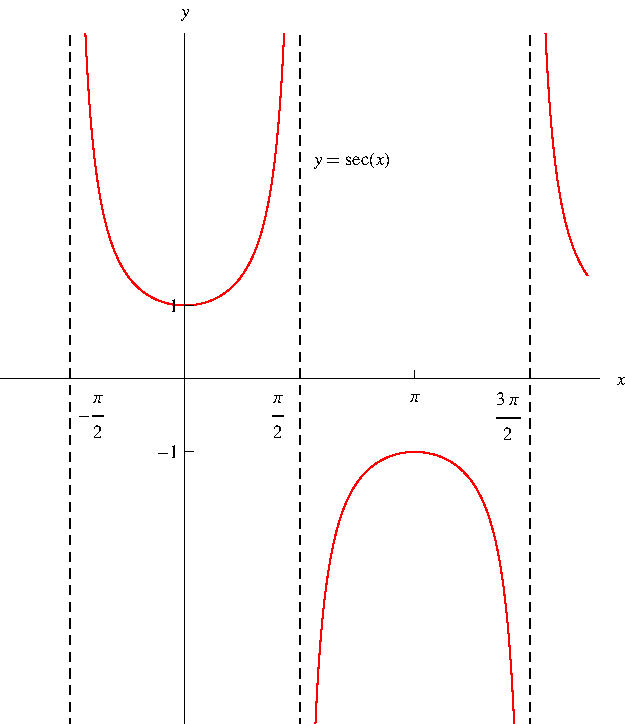
\includegraphics[width=5cm]{inverse-trig/pictures/07-06-seca.pdf}%
}%
\only<2->{%
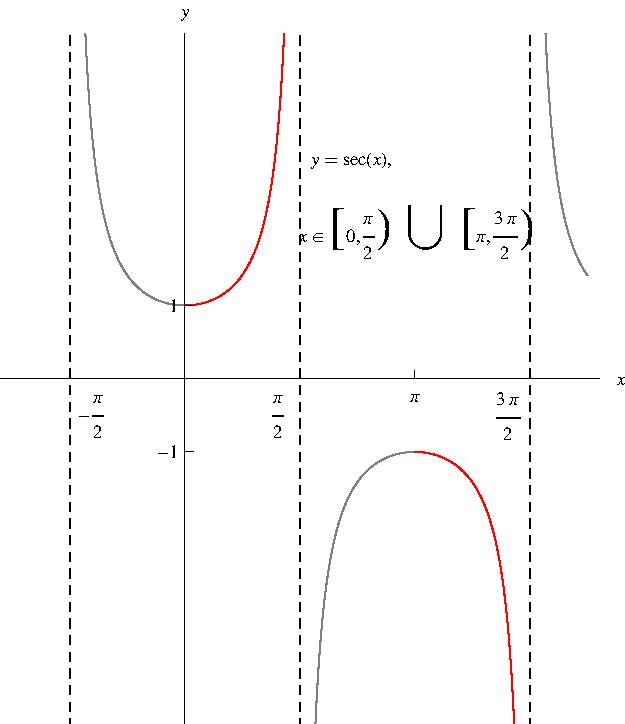
\includegraphics[width=5cm]{inverse-trig/pictures/07-06-secb.pdf}%
}%
\end{frame}

\begin{frame}
Table of derivatives of inverse trigonometric functions: 
\begin{align*}
\frac{\diff}{\diff x} (\arcsin x) & = %
\frac{1}{\sqrt{1-x^2}} &%
\frac{\diff}{\diff x} (\csc^{-1} x) & = %
-\frac{1}{x\sqrt{x^2-1}} \\%
\frac{\diff}{\diff x} (\arccos x) & = %
-\frac{1}{\sqrt{1-x^2}} &%
\frac{\diff}{\diff x} (\sec^{-1} x) & = %
\frac{1}{x\sqrt{x^2-1}} \\%
\frac{\diff}{\diff x} (\arctan x) & = %
\frac{1}{1+x^2} &%
\frac{\diff}{\diff x} (\cot^{-1} x) & = %
-\frac{1}{1+x^2} %
\end{align*}
\end{frame}
% end module inverse-trig-summary

%% begin module integration-by-parts-ex3
\begin{frame}
\alert<4,5,12,13>{Integration by parts:} $\displaystyle \int \alert<6,14>{u} \diff \alert<7,15>{v} = \alert<6 ,14>{ u} \alert<7,15>{v} - \int \alert<7,15>{v} \diff \alert<6,14>{u}.$

\begin{example}

$\begin{array}{rcll|l}
\displaystyle \int t^2\alert<2,3>{ e^t \diff t} \uncover<2->{ &\alert<0>{=}&\displaystyle \int \alert<6>{ t^2} \alert<2,3>{ \diff \left(\fcAnswer{3}{\alert<7>{e^t}}\right) }} \uncover<4->{&& \alert<4,5>{\text{integrate by parts}}}\\
\uncover<4->{&\alert<4>{=}&\displaystyle \fcAnswer{5}{  \alert<6>{t^2}\alert<7>{ e^t} - \int\alert<7>{ e^t} \alert<8,9>{\diff \left(\alert<6>{t^2}\right) }}}\\
\uncover<8->{ &\alert<0>{=}&\displaystyle t^2e^t- \int \alert<10,11>{e^t} \fcAnswer{9}{2t} \alert<8,9,10,11>{ \diff t}}\\
\uncover<10->{&\alert<0>{=}&\displaystyle t^2 e^t - 2 \alert<12,13>{ \int \alert<14>{t} \alert<10,11>{ \diff (\fcAnswer{11}{ \alert<15>{e^t} })}}} \uncover<12->{&&\alert<12,13>{\text{integrate by parts}}}\\
\uncover<12->{&\alert<0>{=}&\displaystyle t^2e^t\alert<17>{-2}\fcAnswer{13}{\left(\alert<14>{t} \alert<15>{e^t}\alert<17>{-} \alert<16>{\int \alert<15>{e^t} \diff \alert<14>{t}} \right)}}\\
\uncover<16->{&\alert<0>{=}&\displaystyle t^2e^t-2te^t\alert<17>{+2}\alert<16>{e^t}+C}
\end{array}
$
\end{example}
\end{frame}
% end module integration-by-parts-ex3


%\begin{frame}
\frametitle{$\sin(\alpha+\beta), \cos(\alpha+\beta)$ via $\sin\alpha, \sin\beta, \cos\alpha, \cos\beta$}
\vskip -0.1cm
\begin{columns}
\column{0.53\textwidth}
\psset{xunit=4cm, yunit=4cm}
\begin{pspicture}(-0.02, -0.1)(1.2,0.8)
\fcBoundingBox{-0.02}{-0.1}{1.2}{0.9}
\tiny%
\pstVerb{%
20 dict begin
/alpha 23 def
/beta 35 def
/pointA {beta cos alpha cos mul 0} def
/pointB {beta cos alpha cos mul beta cos alpha sin mul} def
/pointC {alpha beta add cos alpha beta add sin} def
/pointD {alpha beta add cos 0} def
/pointH {alpha beta add cos alpha beta add cos alpha sin mul alpha cos div} def
/pointQ {alpha beta add cos beta cos alpha sin mul } def
}%
%\only<2->{\pstVerb{/alpha 25 def}}
%\only<3->{\pstVerb{/alpha 30 def}}
%\only<4->{\pstVerb{/alpha 35 def}}
%\only<5->{\pstVerb{/alpha 40 def}}
%\only<6->{\pstVerb{/beta 25 def}}
%\only<7->{\pstVerb{/beta 30 def}}
%\only<8->{\pstVerb{/beta 35 def}}
%\only<9->{\pstVerb{/beta 40 def}}
%\only<10->{\pstVerb{/beta 55 def}}
\uncover<3->{\fcPerpendicular[anglelinewidth=1pt]{[pointC]}{[pointB]}{0.03}}%
\only<handout:0|19>{\fcPerpendicular[anglelinewidth=2pt]{[pointC]}{[pointB]}{0.03}}%
\only<handout:0|20>{\psline[linewidth=2pt, linecolor=orange](! pointC)(! pointB)}%
\only<handout:0|21>{\psline[linewidth=2pt, linecolor=blue](! pointC)(! pointB)}%
\uncover<5->{\fcPerpendicular[anglelinewidth=1pt]{[pointC]}{[pointA]}{0.03}}%
\only<handout:0|17>{\fcPerpendicular[anglelinewidth=2pt]{[pointC]}{[pointA]}{0.03}}%
\only<handout:0|7>{\fcPerpendicular[linewidth=2pt,linecolor=blue, anglelinewidth=1pt]{[pointC]}{[pointA]}{0.03}}%
\uncover<2->{\fcPerpendicular[anglelinewidth=1pt]{[pointB]}{[pointA]}{0.03}}%
\only<handout:0|11,12,15>{\psline[linecolor=blue, linewidth=2pt](! pointB)(! pointA)}%
\uncover<2->{\fcAngleBetweenVectors{[pointA]}{[pointB]}{0.2}{$~~~\alpha$}}%
\uncover<9->{\fcPerpendicular[]{[pointB]}{  [pointH] [pointC]}{0.03}}%
\only<handout:0|2,12,17>{\parametricplot[linewidth=2pt, linecolor=red]{0}{alpha}{t cos 0.2 mul t sin 0.2 mul}}%
\uncover<3->{\fcAngleBetweenVectors{[pointB]}{[pointC]}{0.2}{$~~~~\beta$}}%
\only<handout:0|3,13,21>{\parametricplot[linewidth=2pt, linecolor=red]{alpha}{alpha beta add}{t cos 0.2 mul t sin 0.2 mul}}%
\uncover<2->{%
\psline(0,0)(! pointB)%
\psline(0,0)(! pointA)%
}%
\only<handout:0|12>{\psline[linecolor=orange, linewidth=2pt](! pointB)(0,0)}%
\only<handout:0|13>{\psline[linecolor=green, linewidth=2pt](! pointB)(0,0)}%
%\only<handout:0|7>{\psline[linecolor=green, linewidth=2pt](! pointD)(0,0)}%
\uncover<3->{\psline(0,0)(! pointC)}%
\only<handout:0|4,7,8,13,14,21,22>{\psline[linecolor=orange, linewidth=2pt](0,0)(! pointC)}%
\uncover<2->{\rput[t](0,-0.02){ $O$}}
\uncover<2->{\rput[lt](! pointA){ $A$}}
\uncover<2->{\rput[l](! pointB){ $B$}}
\uncover<3->{\rput[lb](! pointC){ $C$}}%
\uncover<3->{\rput[br](! [pointC] 0.5 \fcVectorTimesScalar \fcArrayToStack ){$\alertNoH{4,8,14,22}{1}~$}}
%\rput[br](! [pointB] 0.5 \fcVectorTimesScalar \fcArrayToStack ){$\cos \beta$}
\uncover<21->{\rput[l](! [pointC] [pointB] \fcVectorPlusVector 0.5 \fcVectorTimesScalar \fcArrayToStack ){$~\alertNoH{22}{\sin \beta} \uncover<handout:0|21>{|OC|}$}}
\uncover<15->{\rput[l](! [pointB] [pointA] \fcVectorPlusVector 0.5 \fcVectorTimesScalar \fcArrayToStack ){$~\alertNoH{15}{\cos \beta\sin \alpha}$}}%
\uncover<23->{\rput[r](! [pointC] [pointQ] \fcVectorPlusVector 0.5 \fcVectorTimesScalar \fcArrayToStack){$ \alertNoH{23}{ \cos\alpha \sin \beta}~~$}}%
\uncover<5->{\rput[t](! pointD -0.02 add){$D$}}%
\uncover<5->{\rput[tl](! pointH){$~~H$}}%
\uncover<9->{\rput[br](! pointQ){$Q~$}}%
\only<handout:0|10,16,23>{\psline[linecolor=cyan, linewidth=2pt](! pointC)(! pointQ)}%
\only<handout:0|20>{\psline[linecolor=green, linewidth=2pt](! pointC)(! pointQ)}%
\only<handout:0|10,11>{\psline[linecolor=blue, linewidth=2pt](! pointQ)(! pointD)}%
\uncover<17>{\rput(! pointH){\fcAngleDegrees[linecolor=blue, linewidth=2pt]{180 alpha add}{270}{0.03}{}}}%
\uncover<17->{\rput(! pointH){\fcAngleDegrees[linecolor=blue]{180 alpha add}{270}{0.03}{}}}%
\uncover<18,19>{\rput(! pointH){\fcAngleDegrees[linecolor= blue, linewidth=2pt]{ alpha}{90}{0.03}{}}}%
\uncover<18->{\rput(! pointH){\fcAngleDegrees[linecolor= blue]{ alpha}{90}{0.03}{}}}%
\uncover<16->{\rput(! pointC){\fcAngleDegrees[linecolor= red]{-90 }{-90 alpha add}{0.1}{}}}%
\only<handout:0|16,19,20>{\rput(! pointC){\fcAngleDegrees[linecolor= red, linewidth=2pt]{-90 }{-90 alpha add}{0.1}{}}}%
\uncover<16->{\rput[lt](! pointC exch 0.01 add exch -0.12 add){$\fcAnswerUncover{16}{19}{\alertNoH{20}{\alpha}}$}}%
\uncover<17->{\rput[tr](!pointH exch 0 add exch -0.07 add){$~~~~~\alertNoH{18}{90^\circ-\alpha}$}}%
\only<handout:0|18,19>{\rput[bl](! pointH exch 0.01 add exch 0.04 add){$~~~\alertNoH{18,19}{90^\circ-\alpha}$}}%
\pstVerb{end}
\end{pspicture}

\noindent $\!\!\!\!
\begin{array}{r@{~}c@{~}l}
\alertNoH{1,26}{\sin (\alertNoH{2}{\alpha}+ \alertNoH{3}{\beta})}& \alertNoH{1}{=} &\displaystyle \fcAnswerUncover{1}{7}{ \frac{|CD|}{\alertNoH{8}{|OC|}}} \uncover<8->{=\alertNoH{10}{|CD|}}\\
\uncover<10->{&\alertNoH{0}{=}& \alertNoH{10}{\alertNoH{11, 15}{|QD |}+ \alertNoH{16,23}{|CQ|}}}\\
\uncover<15->{& \alertNoH{26}{=}& \alertNoH{26}{\alertNoH{15}{\sin \alpha \cos \beta} +\fcAnswerUncover{15}{23}{\cos\alpha \sin \beta}}}\\
\alertNoH{24,25,26}{\cos (\alertNoH{2}{\alpha} +\alertNoH{3}{ \beta })} &\alertNoH{24,25}{=}&\displaystyle \fcAnswerUncover{1 }{25}{ \frac{ |OD|}{|OC|}=|OD|}\\
\uncover<25->{&\alertNoH{25}{=}&\alertNoH{25}{ |OA|-|DA|}}\\
\uncover<25->{&\alertNoH{25,26}{=}& \alertNoH{25,26}{\cos \alpha \cos \beta -\sin\alpha \sin \beta}} \\
\end{array}
$

\column{0.47\textwidth}
$
\begin{array}{r@{~}c@{~}l@{}l@{}|l@{}}
\uncover<11->{\alertNoH{11,15}{|QD|}&\alertNoH{11}{=}&\alertNoH{11,12}{|BA|} &&\!\rectangle DABQ}\\
\uncover<12->{&\alertNoH{12}{=}& \alertNoH{12}{\sin \alpha \alertNoH{13}{|OB|}} &&\!\triangle OAB}\\
\uncover<13->{&\alertNoH{0}{=}&\sin\alpha \alertNoH{13}{\cos\beta \alertNoH{14}{|OC|}} &&\!\triangle OBC}\\
\uncover<14->{&\alertNoH{15}{=}& \alertNoH{15}{\sin\alpha \cos \beta}}\\
\uncover<16->{\alertNoH{16,20,23}{|CQ|}&\alertNoH{20}{=}& \uncover<20->{\alertNoH{20}{\cos \alpha\alertNoH{21}{ |CB|}}  &&\! \triangle CQB}} \\
\uncover<21->{&\alertNoH{0}{=}&\cos \alpha\alertNoH{21,22}{ \sin \beta  |OC|}  &&\! \triangle OBC}\\
\uncover<22->{&\alertNoH{23}{=}& \alertNoH{23}{\cos \alpha \alertNoH{22}{\sin \beta } }} \\
\uncover<25->{|OA|&\alertNoH{0}{=}&\cos \alpha |OB| &&\!\triangle OAB\\
&\alertNoH{0}{=}&\cos \alpha \cos \beta |OC|&&\!\triangle OBC\\
&\alertNoH{0}{=}&\cos \alpha \cos \beta\\
|DA|&\alertNoH{0}{=}&|QB|&&\!\rectangle DABQ\\
&\alertNoH{0}{=}&\sin \alpha |CB| &&\!\triangle CQB\\
&\alertNoH{0}{=}&\sin\alpha \sin\beta|OC|&&\!\triangle OBC\\
&\alertNoH{0}{=}&\sin \alpha \sin \beta\\}
\end{array}
$
\end{columns}

\end{frame}



%% begin module arctan-def
\begin{frame}
\begin{columns}[c]
\column{.5\textwidth}
\ \only<handout:0| -1>{%
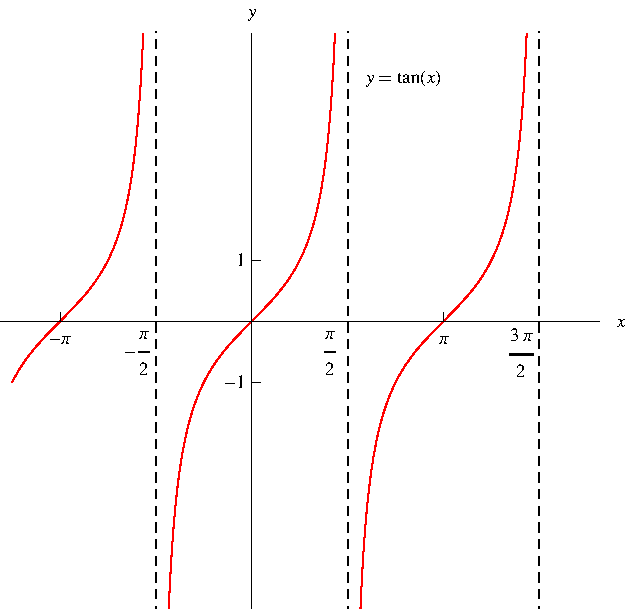
\includegraphics[width=5cm]{inverse-trig/pictures/07-06-arctana.pdf}%
}%
\only<handout:1| 2>{%
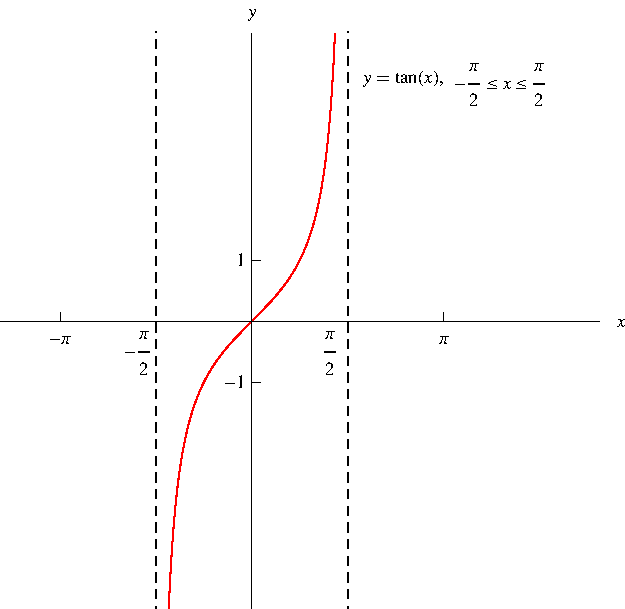
\includegraphics[width=5cm]{inverse-trig/pictures/07-06-arctanb.pdf}%
}%
\only<handout:2| 3->{%
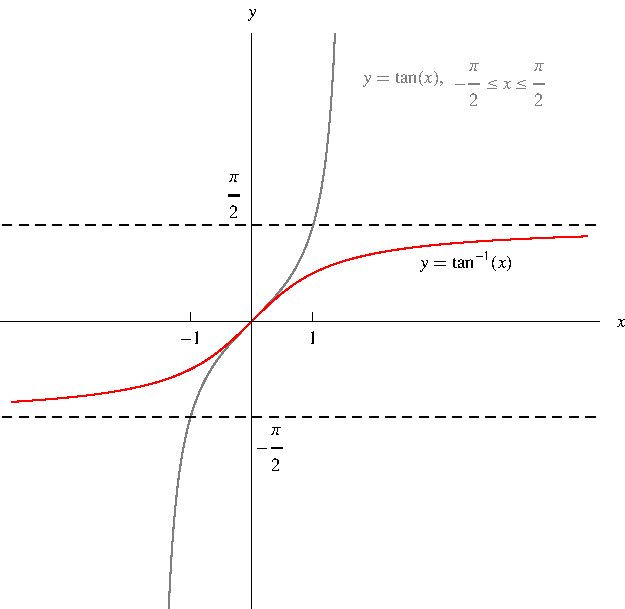
\includegraphics[width=5cm]{inverse-trig/pictures/07-06-arctanc.pdf}%
}%
\column{.5\textwidth}
\begin{itemize}
\item<1->  $\tan x$ isn't one-to-one.
\item<2->  Restrict the domain to $(-\pi /2, \pi /2)$.
\item<3->  The inverse is called $\Arctan$ or $\arctan$.
\item<4->  $\Arctan x = y \Leftrightarrow \tan y = x$ and $-\pi /2 < y < \pi /2$.
\item<5->  \alert<handout:0| 5-6>{Domain of $\Arctan$: \uncover<6-| handout:0>{$(-\infty,\infty)$.}}
\item<5->  \alert<handout:0| 7-8>{Range of $\Arctan$: \uncover<8-| handout:0>{$(-\pi / 2, \pi / 2)$.}}
\item<9->  \alert<handout:0| 9-10>{$\displaystyle \lim_{x\rightarrow \infty} \Arctan x = \uncover<10-| handout:0>{\pi / 2.}$}
\item<9->  \alert<handout:0| 11-12>{$\displaystyle \lim_{x\rightarrow - \infty} \Arctan x = \uncover<12-| handout:0>{- \pi / 2.}$}
\end{itemize}
\end{columns}
\end{frame}
% end module arctan-def



%% begin module parametric-tangents-intro-version2
\begin{frame}
\frametitle{Tangents}
Let $C $ be the curve $C:\left|\begin{array}{rcl}x&=&f(t)\\y&=&g(t)\end{array} \right., t\in [a,b]$.
\begin{definition}
Suppose \alert<4,5>{ $f'(t)$ and $g'(t)$ are not simultaneously equal to $0$.} 
\begin{itemize}
\item  We define $(f'(t), g'(t))$ to be the \emph{tangent vector} to $C$ at $t$.
\item<2->  We define the line passing through $(f(t), g(t))$ with direction vector equal to the tangent vector to be \emph{tangent line} to $C$ at $t$. In other words, the tangent line has equation
\[
(x-f(t))g'(t) =(y-g(t))f'(t)\quad .
\]
\item<3->  We say that the tangent to $C$ at $t$ is vertical if $f'(t)=0$ (\alert<4>{and therefore $g'(t)\neq 0$}).
\end{itemize}
\end{definition}
\uncover<5->{\alert<5->{Note.} When $f'(t)=g'(t)=0$, for curves $C$ with additional properties, natural definition(s) of tangent(s) do exist but are beyond Calc II.}
\end{frame}
\begin{frame}
\begin{example}

\end{example}
\end{frame}

\begin{frame}
Recall $C:\left|\begin{array}{rcl}x&=&\only<1>{f}\only<2->{\alert<2>{x}}(t)\\y&=& \only<1>{g}\only<2->{\alert<2>{y}}(t)\end{array} \right., t\in [a,b]$, tangent vector at $t$ is $(\only<1>{f}\only<2->{\alert<2>{x}}'(t), \only<1>{g}\only<2->{\alert<2>{y}}'(t))$. \uncover<2->{We write informally $\alert<2>{x=x(t)}, \alert<2>{y=y(t)}$ to simplify notation.}

\begin{itemize}
\item<3-> Suppose we could eliminate the parameter $t$ and write $y=F(x)$ for some function $F$ near the point $(x,y)=(x(t), y(t))$. 
\item<4-> Suppose in $x'(t)\neq 0$ for some $t$. 
\uncover<5->{
\[
\begin{array}{rcll|l}
\displaystyle y&=&\displaystyle  F(x) &&\text{apply } \frac{\diff }{\diff t}\\
\displaystyle \frac{\diff y}{\diff t}&=&\displaystyle \frac{\diff} {\diff t} \left(F(x)\right)&&\text{use chain rule}\\
&=&\displaystyle  \frac{\diff F}{\diff x} \frac{\diff x}{\diff t}=\frac{\diff y}{\diff  x} \frac{\diff x}{\diff t} &&\text{divide by } x'(t)\\
\displaystyle \frac{\diff y}{\diff x} &=&\displaystyle  \frac{\frac{\diff y}{\diff t} }{\frac{\diff x}{\diff t}}
\end{array}
\] 
}
\end{itemize}
\begin{observation}
If $\frac{\diff x}{\diff t}\neq 0$, we have $\displaystyle \frac{ \diff y}{ \diff x}= \frac{\frac{\diff y}{\diff t}}{\frac{\diff x}{\diff t}}\quad .
$
\end{observation}
\end{frame}
% begin module parametric-tangents-intro-version2

%% begin module parametric-tangents-ex1
\begin{frame}[t]
\begin{example}
\begin{columns}
\column{0.25\textwidth}
\psset{xunit=0.4cm, yunit=0.4cm}
\begin{pspicture}(-0.9, -2.4)(4.4,2.499997)
\tiny
\fcAxesStandard{-0.650000}{-2.150000}{4.150000}{2.149997}
%Calculator input: plotCurve{}(t^{2}, t^{3}-3 t, -2, 2)
\parametricplot[linecolor=\fcColorGraph, plotpoints=1000]{-2}{2}{t 2.0000000 exp t -3.0000000 mul t 3.0000000 exp add }
\end{pspicture}
\column{0.75\textwidth}
A curve $C$ is defined by $x = t^2, y = t^3 - 3t$.
\end{columns}
\begin{enumerate}
\item Show $C$ traverses $(x,y)=(3,0)$ for two values of $t$; find the tangent slopes for both of these values.
\item Find the points on $C$ where the tangents are horizontal or vertical.
\item Find two intervals where we can write $y$ as a function of $x$.
\item Determine concavity intervals of the functions found in item 3.
\end{enumerate}
\end{example}
\vspace{4cm}
\end{frame}




\begin{frame}[t]
\begin{example}
\begin{columns}
\column{0.25\textwidth}
\psset{xunit=0.4cm, yunit=0.4cm}
\begin{pspicture}(-0.9, -2.4)(4.4,2.499997)
\tiny%
\fcAxesStandard{-0.650000}{-2.150000}{4.150000}{2.149997}%
%Calculator input: plotCurve{}(t^{2}, t^{3}-3 t, -2, 2)
\parametricplot[linecolor=\fcColorGraph, plotpoints=1000]{-2}{2}{t 2.0000000 exp t -3.0000000 mul t 3.0000000 exp add }%
\fcFullDotBlue{3}{0}%
\uncover<15->{%
\psline[linecolor=\fcColorTangent](2,1.732050808)(4,-1.732050808)%
\psline[linecolor=\fcColorTangent](2,-1.732050808)(4,1.732050808)%
}%
\end{pspicture}
\column{0.75\textwidth}
A curve $C$ is defined by \alert<handout:0| 2>{$x = t^2, y = t^3 - 3t$}.
\end{columns}
\begin{enumerate}
\item Show $C$ traverses $(x,y)=(3,0)$ for two values of $t$; find the tangent slopes for both of these values.
\end{enumerate}
\begin{itemize}
\item<2-| alert@3-4>  $3 = \alert<handout:0| 2>{x = t^2}$ \ if \ $t = $ \uncover<4->{$\pm \sqrt{3}$.}
\item<2-| alert@5-6>  $0 = \alert<handout:0| 2>{y = t^3 - 3t} = t(t^2-3)$\  if \ $t = $ \uncover<6->{$0$\  or\  $\pm \sqrt{3}$.}
\item<7->  Therefore the point $(3,0)$ is traversed when $t$ equals $\sqrt{3}$ or $-\sqrt{3}$.
\item<8-> $ \uncover<8->{ \frac{\diff y}{\diff x} = \frac{\alert<handout:0| 9-10>{\diff y / \diff t}}{\alert<handout:0| 11-12>{\diff x / \diff t}} %
} \uncover<9->{= \frac{\alert<handout:0| 10>{\uncover<10->{3t^2-3 }}}{\alert<handout:0| 12>{\uncover<12->{2t }}}}$\uncover<12->{\quad .}
\item<13->
Plug in $t = \pm \sqrt{3}$:
$\displaystyle
\uncover<13->{%
\frac{\diff y}{\diff x} _{|t = \pm \sqrt{3}} = \frac{3(\pm \sqrt{3})^2 - 3}{2(\pm \sqrt{3})} = %
}%
\uncover<14->{%
\pm \frac{6}{2\sqrt{3}} = \pm \sqrt{3}%
}%
$
\uncover<15->{%
Therefore the tangents at $(3,0)$ have slopes $\pm \sqrt{3}$.
}%
\end{itemize}
\end{example}
\vspace{4cm}
\end{frame}

\begin{frame}[t]
\begin{example}
\begin{columns}
\column{0.25\textwidth}
\psset{xunit=0.4cm, yunit=0.4cm}
\begin{pspicture}(-0.9, -2.4)(4.4,2.499997)
\tiny
\fcAxesStandard{-0.650000}{-2.150000}{4.150000}{2.149997}
%Calculator input: plotCurve{}(t^{2}, t^{3}-3 t, -2, 2)
\parametricplot[linecolor=\fcColorGraph, plotpoints=1000]{-2}{2}{t 2.0000000 exp t -3.0000000 mul t 3.0000000 exp add }
\uncover<6->{%
\fcFullDotBlue{1}{2}
\fcFullDotBlue{1}{-2}
\psline[linecolor=\fcColorTangent](0.1,2)(1.9,2)
\psline[linecolor=\fcColorTangent](0.1,-2)(1.9,-2)
}%
\uncover<10->{%
\fcFullDotBlue{0}{0}
\psline[linecolor=\fcColorTangent](0,-1)(0,1)
}%
\end{pspicture}
\column{0.75\textwidth}
A curve $C$ is defined by $x = t^2, y = t^3 - 3t$.
\end{columns}
\begin{enumerate}
\setcounter{enumi}{1}
%\item  Show that $C$ has two tangents at $(3,0)$ and find their slopes.
\item  Find the points on $C$ where the tangents are horizontal or vertical.
%\item  Determine where the curve is concave up or down.
\end{enumerate}
\begin{columns}[t]
\column{.5\textwidth}
Horizontal tangent:
\abovedisplayskip=0pt
\belowdisplayskip=0pt
\begin{eqnarray*}
\frac{\diff y}{\diff t} & = & 0\\
\uncover<2->{%
3t^2 - 3%
}%
& \uncover<2->{ = } & %
\uncover<2->{%
0
}\\%
\uncover<3->{%
3(t^2 - 1)%
}%
& \uncover<3->{ = } & %
\uncover<3->{%
0
}\\%
\uncover<4->{%
t%
}%
& \uncover<4->{ = } & %
\uncover<4->{%
\pm 1%
}%
\end{eqnarray*}
\uncover<5->{$\frac{\diff x}{\diff t} \neq 0$ when $t = \pm 1$, so there are horizontal tangents when $t = \pm 1$.}

\uncover<6->{%
The points are $(1, 2)$ and $(1, -2)$.
}%
\column{.5\textwidth}
Vertical tangent:
\abovedisplayskip=0pt
\belowdisplayskip=0pt
\begin{eqnarray*}
\frac{\diff x}{\diff t} & = & 0\\
\uncover<7->{%
2t%
}%
& \uncover<7->{ = } & %
\uncover<7->{%
0%
}\\%
\uncover<8->{%
t%
}%
& \uncover<8->{ = } & %
\uncover<8->{%
0%
}%
\end{eqnarray*}
\uncover<9->{$\frac{\diff y}{\diff t} \neq 0$ when $t =  0$, so there is a vertical tangent when $t = 0$.}

\uncover<10->{%
The points is $(0,0)$.
}%
\end{columns}
\end{example}
\vspace{4cm}
\end{frame}



\begin{frame}[t]
\begin{example} %[Example 1, p. 667]
\begin{columns}
\column{0.25\textwidth}
\psset{xunit=0.4cm, yunit=0.4cm}
\begin{pspicture}(-0.9, -2.4)(4.4,2.499997)
\tiny
\fcAxesStandard{-0.650000}{-2.150000}{4.150000}{2.149997}
\uncover<1-4,6->{%
%Calculator input: plotCurve{}(t^{2}, t^{3}-3 t, -2, 2)
\parametricplot[linecolor=\fcColorGraph, plotpoints=1000]{-2}{0}{t 2.0000000 exp t -3.0000000 mul t 3.0000000 exp add }%
}%
\uncover<1-5>{%
\parametricplot[linecolor=\fcColorGraph, plotpoints=1000]{0}{2}{t 2.0000000 exp t -3.0000000 mul t 3.0000000 exp add }%
}%
\end{pspicture}
\column{0.75\textwidth}
A curve $C$ is defined by $x = t^2, y = t^3 - 3t$.
\end{columns}
\begin{enumerate}
\setcounter{enumi}{2}
%\item  Show that $C$ has two tangents at $(3,0)$ and find their slopes.
%\item  Find the points on $C$ where the tangents are horizontal or vertical.
\item  Find two intervals where we can write $y$ as a function of $x$.
\end{enumerate}
\uncover<2->{From $x=t^2$ we have that $t=\pm \sqrt{x}$.} \uncover<3->{Therefore, when $t>0$, we have that $t=\sqrt{x}$.} \uncover<4->{Since that determines uniquely $t$ via $x$, this means that for $t>0$  $y$ is a function of $x$.} \uncover<5->{In other words, for $t>0$, the curve satisfies the vertical line test. } \uncover<6->{Similarly we conclude that when $t<0$, $y$ is a function of $x$.}
\end{example}
\vspace{5cm}
\end{frame}

\begin{frame}[t]
\begin{example} %[Example 1, p. 667]
\begin{columns}
\column{0.25\textwidth}
\psset{xunit=0.4cm, yunit=0.4cm}
\begin{pspicture}(-0.9, -2.4)(4.4,2.499997)
\tiny
\fcAxesStandard{-0.650000}{-2.150000}{4.150000}{2.149997}
\uncover<1-11,13->{%
%Calculator input: plotCurve{}(t^{2}, t^{3}-3 t, -2, 2)
\parametricplot[linecolor=\fcColorGraph, plotpoints=1000]{-2}{0}{t 2.0000000 exp t -3.0000000 mul t 3.0000000 exp add }%
}%
\uncover<1-12>{%
\parametricplot[linecolor=\fcColorGraph, plotpoints=1000]{0}{2}{t 2.0000000 exp t -3.0000000 mul t 3.0000000 exp add }%
}%
\end{pspicture}
\column{0.75\textwidth}
A curve $C$ is defined by $x = t^2, y = t^3 - 3t$.
\end{columns}
\begin{enumerate}
\setcounter{enumi}{3}
\item  Determine the concavity intervals of the functions found in item 3.
\end{enumerate}
\uncover<2->{Find the second derivative:}%

$\begin{array}{rcl}
\displaystyle \uncover<2->{%
\frac{\diff^2 y}{\diff x^2}%
}%
& \uncover<2->{ = } &%
\displaystyle \uncover<2->{%
\frac{\frac{\diff}{\diff t}\left( \alert<handout:0| 3-4>{\frac{\diff y}{\diff x}}\right)}{\alert<handout:0| 5-6>{\frac{\diff x}{\diff t}}}%
}  \uncover<3->{ = }  \uncover<3->{%
\frac{\frac{\diff}{\diff t}\left( \alert<handout:0| 3-4,7>{\uncover<4->{\frac{3t^2-3}{2t}}}\right)}{\alert<handout:0| 5-6>{\uncover<6->{2t}}}%
}\\%
& \uncover<7->{ = } &\displaystyle
\uncover<7->{%
\frac{\alert<handout:0| 8-9>{\frac{\diff}{\diff t}\left( \alert<handout:0| 7>{\frac{3}{2}\left( t - \frac{1}{t}\right)}\right)}}{2t}%
}  \uncover<8->{ = }  \uncover<8->{%
\frac{\alert<handout:0| 8-9>{\uncover<9->{\frac{3}{2} + \frac{3}{2t^2} }}}{2t}%
}\\%
& \uncover<10->{ = } &\displaystyle
\uncover<10->{%
\frac{\frac{3t^2 + 3}{2t^2}}{2t}%
}  \uncover<11->{ = } \uncover<11->{%
\frac{3(t^2 + 1)}{4t^3}%
}%
\end{array}
$

\uncover<12->{%
Therefore $y$ as a function of $x$ (which is a function of $t$) is concave up when $t > 0$}\uncover<13->{ and concave down when $t < 0$.}%
\end{example}
\vspace{4cm}
\end{frame}
% end module parametric-tangents-ex1


%\begin{frame}
\begin{example}
\begin{columns}
\column{0.35\textwidth}
\begin{pspicture}(-2.1,-2.1)(2.1,2.1)
\tiny
\fcBoundingBox{-2.2}{-2.2}{2.2}{2.2}
\fcAxesStandard{-2}{-2}{2}{2}
\fcLabels[$\Re$][$\Im$]{2}{2}
\end{pspicture}
\column{0.65\textwidth}
Plot the number $z$. Write $z$ in polar form, using the principal value of the argument of $z$ (polar angle). 

Recall that $\theta$ is the principal argument $\Rightarrow$ $\theta\in (-\pi,\pi]$.

\begin{tabular}{c|c|c|c}
$z$ & $|z|$ & $\theta$ & $|z|(\cos\theta +i\sin \theta)$\\\hline
$1$ & 1 & $0 $ & $\cos 0+i\sin 0$\\
$i$ & 1 & $\frac{\pi}{2} $& $\cos\left(\frac{\pi}{2}\right)+i\sin\left(\frac{\pi}{2}\right)$   \\
$-1$ & $1$&$\pi$&$\cos \pi +i\sin\pi$ \\
$-i$ & $1$&$-\frac{\pi}{2}$& $\cos\left(-\frac{\pi}{2}\right)+ i \sin \left(- \frac{\pi}{2}\right)$  \\
\end{tabular} 
\end{columns}

\end{example}
\end{frame}
%



\begin{frame}
\begin{example}
\begin{columns}
\column{0.35\textwidth}
\begin{pspicture}(-2.1,-2.1)(2.1,2.1)
\tiny
\fcBoundingBox{-2.2}{-2.2}{2.2}{2.2}
\fcAxesStandard{-2}{-2}{2}{2}
\fcLabels[$\Re$][$\Im$]{2}{2}
\end{pspicture}
\column{0.65\textwidth}
Plot the number $z$. Write $z$ in polar form, using the principal value of the argument of $z$ (polar angle). 

Recall that $\theta$ is the principal argument $\Rightarrow$ $\theta\in (-\pi,\pi]$.
\end{columns}
\begin{tabular}{c|c|c|c}
$z$ & $|z|$ & $\theta$ & $|z|(\cos\theta +i\sin \theta)$\\\hline
$\frac{1}{2}+\frac{\sqrt{3}}{2}i$&$1$& $\frac{\pi}{3}$& $\cos \left( \frac{ \pi}{3}\right)+ i \sin \left( \frac{\pi }{3} \right) $\\
$1+i$&$2$&$\frac{\pi}{4}$& $2\left( \cos\left(\frac{\pi}{4} \right)+ i \sin \left( \frac{\pi}{4}\right)\right) $\\
$1-i$&$2$&$-\frac{\pi}{4}$& $2\left( \cos\left(-\frac{\pi}{4} \right)+ i \sin \left( -\frac{\pi}{4}\right)\right) $\\
$-\sqrt{3}-i $&$2$& $-\frac{2\pi}{3}$&$ 2\left( \cos \left( \frac{ 2\pi}{3} \right)+ i \sin \left( \frac{2\pi }{3} \right) \right) $\\
$\frac{3}{5}+\frac{4}{5}i$&$5$&$\Arctan\left(\frac{4}{3}\right)$& $5\left(\cos \left(\Arctan\left(\frac{4}{3}\right)\right)+i \sin \left(\Arctan\left(\frac{4}{3}\right)\right) \right) $ \\
\end{tabular}
\end{example}
\end{frame}



%\begin{frame}
\frametitle{Geometric interpretation of complex multiplication}
\begin{columns}
\column{0.35\textwidth}

\begin{pspicture}(-0.5, -0.5)(3,3)
\tiny
\fcAxesStandard{-0.5}{-0.5}{2.5}{2.5}
\fcLabels[$\Re$][$\Im$]{2.5}{2.5}
\pstVerb{10 dict begin /erho 2 def /esigma 1.4 def /alpha 10 def /beta 50 def }%
\uncover<handout:0|14->{%
\parametricplot[linecolor=gray, linewidth=0.5pt]{-10}{120}{t cos t sin}%
\rput[t](1,-0.1){$~~1$}%
}%
\only<handout:0|15>{\pstVerb{/esigma 1.2 def}}%
\only<handout:0|16>{\pstVerb{/esigma 1 def}}%
\only<handout:0|17>{\pstVerb{/esigma 0.8 def}}%
\only<handout:0|19>{\pstVerb{/beta 40 def}}%
\only<handout:0|20>{\pstVerb{/beta 30 def}}%
\only<handout:0|21>{\pstVerb{/beta 20 def}}%
\uncover<handout:0|14->{\parametricplot[linecolor=gray, linewidth=0.5pt, linestyle=dashed]{5}{85}{t cos erho mul t sin erho mul} }%
\pstVerb{
/zx erho alpha cos mul def 
/zy erho alpha sin mul def 
/wx esigma beta cos mul def 
/wy esigma beta sin mul def 
/zwx erho esigma mul alpha beta add cos mul def 
/zwy erho esigma mul alpha beta add sin mul def 
}%
\fcFullDot{wx}{wy}
\fcFullDot{zx}{zy}
\psline(0,0)(! zx zy)
\psline(0,0)(! wx wy)
\uncover<handout:0|3,12>{\psline[linecolor=red, linewidth=2pt](0,0)(! zx zy)}
\uncover<handout:0|4,12>{\psline[linecolor=red, linewidth=2pt](0,0)(! wx wy)}
\rput[tl](! zx zy){$~z$}
\rput[tl](! wx wy){$~w$}
\uncover<6->{\fcAngleDegrees{0}{alpha}{0.7}{$\alert<handout:0|6>{\alpha} $}}
\uncover<7->{\fcAngleDegrees{0}{beta}{0.3}{$\alert<handout:0|7>{\beta}$}}
\uncover<handout:0|6,10,11>{\fcAngleDegrees[linewidth=2pt, linecolor=red ] {0}{alpha}{0.7}{}}
\uncover<handout:0|7>{\fcAngleDegrees[linewidth=2pt, linecolor=red ] {0}{beta}{0.3}{}}
\uncover<9->{
\fcFullDot{zwx}{zwy}
\rput[tl](! zwx zwy){$~~ zw$}
\psline(0,0)(!zwx zwy)
}
\uncover<handout:0|12>{\psline[linewidth=2pt, linecolor=red ](0,0)(!zwx zwy)}
\uncover<10->{
\fcAngleDegrees{alpha}{alpha beta add}{0.8}{$\beta$}
}
\uncover<handout:0|10,11>{
\fcAngleDegrees[linewidth=2pt, linecolor=red ]{alpha}{alpha beta add}{0.8}{$\beta$}
}
\pstVerb{end}
\end{pspicture}

\column{0.65\textwidth}
\begin{itemize}
\item Let $z,w\neq 0 $ \uncover<2->{and let 

\hfil $\alert<12>{ \alert<3>{ |z| =e^\rho},\quad \alert<4>{ |w|=e^\sigma}}.$
}
\item<5-> Let $\alpha,\beta$ be arguments of $z,w$. 
$
\begin{array}{rcl}
z&=& e^{\rho}(\cos \alert<handout:0|6>{\alpha} + i \sin \alert<handout:0|6>{\alpha} )=e^{\rho +i\alpha} \\
w&=& e^{\sigma}(\cos \alert<handout:0|7>{\beta} +i\sin \alert<handout:0|7>{\beta} )=e^{\sigma +i\beta} .\end{array} 
$
\end{itemize}
\end{columns}
\uncover<8->{%
\begin{theorem}[Summary]
$\begin{array}{rcl}
\alert<9,10>{z w} &=& \alert<12>{e^\rho} ( \cos\alpha+ i\sin\alpha) \alert<12>{e^\sigma} ( \cos \beta +i\sin \beta )\\ &=&e^{\rho+i\alpha}e^{\sigma+i\beta} =e^{\rho+\sigma +i(\alpha+\beta)}\\
&=& \alert<12>{e^{\rho+\sigma} }(\alert<10>{ \cos (\alpha+\beta)+i\sin (\alpha+\beta)} )  .\end{array}$
\end{theorem}
}%
\begin{itemize}
\item<10-> The argument (polar angle) of $zw$ is $\alert<10>{\alpha+\beta} $.
\item<11-> $\Rightarrow$ Multiplying complex numbers adds arguments (polar angles).
\item<12-> Multiplying complex numbers multiplies absolute values.
\item<13-> \alert<13-17>{What happens to $zw$ when we change $|w|$?} \uncover<18->{ \alert<18-21>{When we change $\beta$?} }
\end{itemize}
\end{frame}
%\begin{frame}[t]
\vskip -0.5cm
\begin{columns}[t]
\column{0.5\textwidth}
\begin{definition}[Exponent, Def. II]
$e^{z}=e(z)=\sum\limits_{n=0}^{\infty}\frac{z^n}{n!}$.
\end{definition}
\column{0.5\textwidth}
\uncover<2->{
\begin{definition}[Polar form]
$|z|=e^{\rho}$, $z=e^{\rho}(\cos \theta+i\sin \theta)$  \vphantom{$\sum\limits_{n=0}^{\infty}\frac{z^n}{n!}$}
\end{definition}
}
\end{columns}
\begin{itemize}
\item<1-> For the duration of this slide, assume Definition II of exponent.
\item<3-> In preceding slides/lectures, by algebraic manipulations of series, we showed that $e(z) e(w)= e^{z} e^{w} = e^{z+w}=e(z+w)$.
\uncover<4->{
\begin{theorem}
$\sin (\alpha+\beta)=\sin \alpha\cos \beta+i\sin \beta \cos \alpha$

$\cos (\alpha+\beta)=\cos\alpha\cos \beta-\sin \alpha\sin \beta$, \quad \quad where $\alpha,\beta\in \mathbb R$
\end{theorem}

\begin{proof}
\small
$\begin{array}{r@{~}c@{~}l}
\uncover<5->{ \alertNoH{10}{\cos (\alpha+\beta)} +i \alertNoH{11}{ \sin (\alpha+\beta)} &=& e^{i(\alpha+ \beta)}} \uncover<6->{ = e^{i\alpha+ i\beta}} \uncover<7->{ =e^{ i \alpha }e^{i\beta}}\\
\uncover<8->{&=&(\cos \alpha +i \sin \alpha)(\cos \beta +i\sin \beta)} \\
\uncover<9->{&=& \alertNoH{10}{(\cos \alpha\cos \beta- \sin\alpha \sin \beta )} \\
&&+ i\alertNoH{11}{( \cos \alpha\sin \beta +\sin\alpha\cos \beta)}.}
\end{array}$

\uncover<10->{Compare \alertNoH{10}{real} and \alertNoH{11}{imaginary} part to get the desired trig identities.}
\end{proof}
}
\end{itemize}
\end{frame}


%\begin{frame}
\begin{columns}
\column{0.4\textwidth}
\uncover<4->{
\begin{pspicture}(-2,-2)(2,2)
\tiny
\fcAxesStandard{-1.3}{-1.3}{2}{2}
\fcLabels[\Re][\Im]{2}{2}
\uncover<7->{%
\psparametricplot{0}{360}{t cos t sin}%
}%
\rput[br](-0.03,1.03){$i$}
\rput[tl](1.1,-0.1){$1$}
\fcFullDot{0}{1}
\fcFullDot{1}{0}
\uncover<8->{\fcAngle{0}{1.047197551}{0.1}{$\theta$}}%
\uncover<6->{%
\psline(0,0)(! 0.5 3 sqrt 2 div)%
\psline[linestyle=dotted](0,0)(! 1 3 sqrt)%
}%
\rput(1.1,1.81){$~~z$}
\fcFullDot{1}{3 sqrt}
\uncover<5->{%
\fcFullDot{0.5}{3 sqrt 2 div}%
\rput[b](0.47,1){$\frac{z}{|z|}$}%
}%
\uncover<handout:0|5>{%
\psline[linewidth=2pt, arrows=->, linecolor=red](0,0)(! 1 3 sqrt )%
}%
\uncover<9->{\fcPerpendicular{[0.5 3 sqrt 2 div]}{[0 0 ] [1 0]}{0.1}}%
\uncover<handout:0|10>{\psline[linecolor=red, linewidth=2pt](0,0)(0.5, 0)}%
\uncover<handout:0|11>{\psline[linecolor=red, linewidth=2pt](! 0.5 3 sqrt 2 div)(0.5, 0)}%
\end{pspicture}
}%
\column{0.6\textwidth}
\uncover<12->{
\begin{theorem}[Euler's formula]
$e^{i\theta}=\cos \theta+i\sin \theta$.
\end{theorem}
} 
\begin{lemma}
$\alert<handout:0|1>{\left|\frac{z}{|z|}\right| } \uncover<2->{\alert<2>{=\frac{|z|}{|z|}}} \uncover<3->{ \alert<3>{ =1 }.}$
\end{lemma}
\end{columns}
\begin{itemize}
\item<4-> Let $z=x+iy$ be a non-zero complex number.
\item<5-> Then $0$, $z$, $\frac{z}{|z|}$ lie on a ray \uncover<7->{and $\frac{z}{|z|}$ lies on the unit circle.}
\item<8-> Let $\theta$ - angle between the real axis and the ray between $0$ and $z$.
\item<9-> Then $\alert<15>{\frac{z}{|z|}= \alert<10>{\cos \theta} +i \alert<11>{\sin \theta}}$.
\item<12-> This gives a geometric proof/motivation for Euler's formula when $\theta $ a real number. \uncover<13->{Euler's f-la does hold over all complex numbers.}
\item<14-> Let $\alert<16>{\rho = \ln |z|}= \ln \sqrt{x^2+y^2}=\frac{1}{2}\ln(x^2+y^2)$.
\item<15-> Then $\alert<15>{z=\alert<16>{|z|}(\cos\theta+i\sin\theta)}\uncover<16->{= \alert<16>{ e^{\rho}}( \cos \theta +i\sin \theta)}$.
\end{itemize}
\uncover<17->{
\begin{definition}
Let $z\neq 0$. Then $z=e^{\rho}(\cos\theta+i\sin \theta)$ is called polar form of $z $.
\end{definition}
}
\end{frame}
%\begin{frame}
Let $u=a+bi$, $v=c+di$, $v\neq 0$.
\begin{example}[Complex number division]
$\begin{array}{rcll|l}
\displaystyle\frac{u}{v}&\uncover<1->{=}& \displaystyle\frac{a+bi}{c+di}~~~~~~~~~~~~~~~~~~~~~~~~~~\\
&\uncover<1->{=}&\displaystyle \frac{(a+bi)}{(c+di)}\frac{(c-di)}{(c-di)} & & \begin{array}{l}
\text{Multiply and divide } \\
\text{by complex conjugate }\\
\text{of denominator}
\end{array}
\\
&\uncover<1->{=}&\displaystyle \frac{(a+bi)(c-di)}{c^2-(di)^2}\\
&\uncover<1->{=}&\displaystyle \frac{ac-adi+cbi-bdi^2}{c^2+d^2}\\
&\uncover<1->{=}&\displaystyle \frac{ac+bd+(bc-ad)i}{c^2+d^2}\\
&\uncover<1->{=}&\displaystyle \frac{ac+bd}{c^2+d^2}+\frac{(bc-ad)}{c^2+d^2}i\\
\end{array}
$
\end{example}
\begin{definition}[Complex number division]
The quotient $\frac{u}{v}$, $v\neq 0$ is defined via the formula above.
\end{definition}
\vskip 10cm
\end{frame}
\end{document}
